%%%%%%%%%%%%%%%%%%%%%%%%%%%%%%%%%%%%%%%%%%%%%%%%%%%%%%%%%%%%%%%%%%%%
%% I, the copyright holder of this work, release this work into the
%% public domain. This applies worldwide. In some countries this may
%% not be legally possible; if so: I grant anyone the right to use
%% this work for any purpose, without any conditions, unless such
%% conditions are required by law.
%%%%%%%%%%%%%%%%%%%%%%%%%%%%%%%%%%%%%%%%%%%%%%%%%%%%%%%%%%%%%%%%%%%%

\documentclass[
  digital, %% This option enables the default options for the
           %% digital version of a document. Replace with `printed`
           %% to enable the default options for the printed version
           %% of a document.
  table,   %% Causes the coloring of tables. Replace with `notable`
           %% to restore plain tables.
  lof,     %% Prints the List of Figures. Replace with `nolof` to
           %% hide the List of Figures.
  lot,     %% Prints the List of Tables. Replace with `nolot` to
           %% hide the List of Tables.
  %% More options are listed in the user guide at
  %% <http://mirrors.ctan.org/macros/latex/contrib/fithesis/guide/mu/sci.pdf>.
]{fithesis3}
%% The following section sets up the locales used in the thesis.
\usepackage[resetfonts]{cmap} %% We need to load the T2A font encoding
\usepackage[T1,T2A]{fontenc}  %% to use the Cyrillic fonts with Russian texts.
\usepackage[
  main=czech, %% By using `czech` or `slovak` as the main locale
                %% instead of `english`, you can typeset the thesis
                %% in either Czech or Slovak, respectively.
  german, russian, czech, slovak %% The additional keys allow
]{babel}        %% foreign texts to be typeset as follows:
%%
%%   \begin{otherlanguage}{german}  ... \end{otherlanguage}
%%   \begin{otherlanguage}{russian} ... \end{otherlanguage}
%%   \begin{otherlanguage}{czech}   ... \end{otherlanguage}
%%   \begin{otherlanguage}{slovak}  ... \end{otherlanguage}
%%
%% For non-Latin scripts, it may be necessary to load additional
%% fonts:
\usepackage{paratype}
\def\textrussian#1{{\usefont{T2A}{PTSerif-TLF}{m}{rm}#1}}
%%
%% The following section sets up the metadata of the thesis.
\thesissetup{
    date          = \the\year/\the\month/\the\day,
    university    = mu,
    faculty       = sci,
    department    = Ústav chemie,
    departmentEn  = Department of Mathematics and
                    Statistics,
    programme     = Chemie,
    programmeEn   = Chemistry,
    field         = Chemie,
    fieldEn       = Chemistry,
    type          = bc,
    author        = Petra Hrozková,
    gender        = f,
    advisor       = doc. Mgr. M. Munzarová Dr. rer. nat ,
    title         = Studium vlivu koordinačního prostředí atomů Si a P na tvorbu SiO$_6$ center metodami EHT a DFT,
    TeXtitle      = Studium vlivu koordinačního prostředí atomů Si a P na tvorbu SiO$_6$ center metodami EHT a~DFT,
    titleEn       = A combined EHT/DFT study of Si and P coordination environment influence on the creation of SiO6 centers,
    TeXtitleEn    = The Principles of the Typesetting of
                    Mathematics in \TeX: the Program,
    keywords      = {klíčové slovo 1, klíčové slovo 2, ...},
    TeXkeywords   = {klíčové slovo 1, klíčové slovo 2, \ldots},
    keywordsEn    = {keyword1, keyword2, ...},
    TeXkeywordsEn = {keyword1, keyword2, \ldots},
}
\thesislong{abstract}{
    This is the abstract of my thesis, which can

    span multiple paragraphs.
}
\thesislong{abstractEn}{
    This is the English abstract of my thesis, which can

    span multiple paragraphs.
}
\thesislong{thanks}{
    This is the acknowledgement for my thesis, which can

    span multiple paragraphs.
}
%% The following section sets up the bibliography.
\usepackage{csquotes}
\usepackage[              %% When typesetting the bibliography, the
  backend=biber,          %% `numeric` style will be used for the
  style=numeric,          %% entries and the `numeric-comp` style
  citestyle=numeric-comp, %% for the references to the entries. The
  sorting=none,           %% entries will be sorted in cite order.
  sortlocale=auto         %% For more unformation about the available
]{biblatex}               %% `style`s and `citestyles`, see:
%% <http://mirrors.ctan.org/macros/latex/contrib/biblatex/doc/biblatex.pdf>.
\addbibresource{example.bib} %% The bibliograpic database within
                          %% the file `example.bib` will be used.
\usepackage{makeidx}      %% The `makeidx` package contains
\makeindex                %% helper commands for index typesetting.
%% These additional packages are used within the document:
\usepackage{paralist}
\usepackage{amsmath}
\usepackage{amsthm}
\usepackage{amsfonts}
\usepackage{url}
\usepackage{menukeys}
\usepackage[version=3]{mhchem}
\usepackage{braket}
\usepackage{subfigure}
\begin{document}
\chapter{Úvod}
Fosfosilikátové sloučeniny mají široké využití jako pokročilé technologické materiály. Jejich stabilní Brönstedovská kyselost za zvýšené teploty je klíčovou vlastností pro využití v palivových článcích a v heterogenní katalýze.\cite{korotcenkov2013handbook}\cite{Fougret2001295} V roce 2015 byla A. Stýskalíkem a spoluautory publikována originální syntéza mezoporózních  nanokrystalických  fosfosilikátů a hybridních anorganicko-organických materiálů pomocí nehydrolytických kondenzačních reakcí založených na esterové eliminaci.\cite{1306716} Jako prekurzory sloužily v případě fosfosilikátů octan křemičitý a tris(trimethylsilyl)ester kyseliny fosforečné. Zatímco posledně jmenované prekurzory poskytly mikroporózní gely se strukturními jednotkami \ce{SiO6}, zavedení organických skupin ve formě různých alkyl/arylacetoxysilanů indukovaly strukturní  a stavební změny vedoucí k neporózní, hybridním silikofosfátovým sklům.\cite{1316862} Tyto drastické změny vlastností byly připsány snížení zesíťovací kapacity křemíku. Organo-substituovaná křemíková centra navíc prokazovala zřejmě nedostatečnou Lewisovskou kyselost k získání hexakoordinace, neboť sterické překážky nehrály ve vzniku \ce{SiO6} center významnější roli.  Dále bylo pozorováno, že přítomnost skupin \ce{SiO6} je spojená s přítomností mikropórů, zatímco pokud tyto skupiny absentují, tak jsou vzorky mesoporézní.
Vzhledem k těmto pozorováním, jakož i obecné zajímavosti problému aktivace křemíku k tvorbě hypervalentních struktur,\cite{rendler2005hypervalent} se jeví jako užitečné studovat vliv prekurzorů na schopnost tvorby center \ce{SiO6} také teoreticky, konkrétně metodami kvantové chemie. Ty totiž poskytují detailní charakterizaci strukturně-elektronových parametrů prekurzorů i výsledných systémů, která by mohla interpretovat tendenci k hypervalenci křemíku v konkrétním systému. Jako téma této bakalářské práce byl zvoleno studium nejjednodušších možných fosfátových prekurzorů využitých v minulosti k syntéze silikofosfátů, konkrétně molekul \ce{POCl3}, \ce{PO(OH)3}, a \ce{PO(OCH3)3}. Elektronová struktura těchto systémů byla studována pomocí Rozšířené Hückelovy metody v implementaci programu C.A.C.A.O.\cite{cacao}. Práce se zaměřuje na porovnání vazebných charakteristik jednotlivých sloučenin z této trojice z hlediska orbitálních interakcí, přičemž nejdůležitějšími zkoumanými semikvantitativními parametry je  vzdálenost energií nejvyššího obsazeného a nejnižšího neobsazeného molekulového orbitalu (tzv. HOMO-LUMO mezera) a velikost energie odpovídající středu tohoto intervalu. Zmíněné parametry jsou totiž v rámci teorie HSAB (\uv{Hard and Soft Acids and Bases}) spojovány s charakterizací tvrdosti a měkkosti Lewisovských kyselin a bazí a jejich reaktivitou.[odkaz] Naším cílem bylo, prostřednictvím porovnání nejjednodušších možných fosfátových prekurzorů, navrhnout strategii pro porozumění elektronové struktuře složitějších prekurzorů využívaných v konkrétních syntézách, např. tris(trimethylsilyl)fosfátu využívaného v syntéze A. Stýskalíka. Z pohledu křemičitanových prekurzorů se podobnému úkolu věnuje bakalářská práce Petry Hrozkové. [odkaz]
\begin{otherlanguage}{czech}

\begin{figure}[h!]
\caption{Silikofosfátová síť. \cite{Styskalik2015thesis} }
  \center
  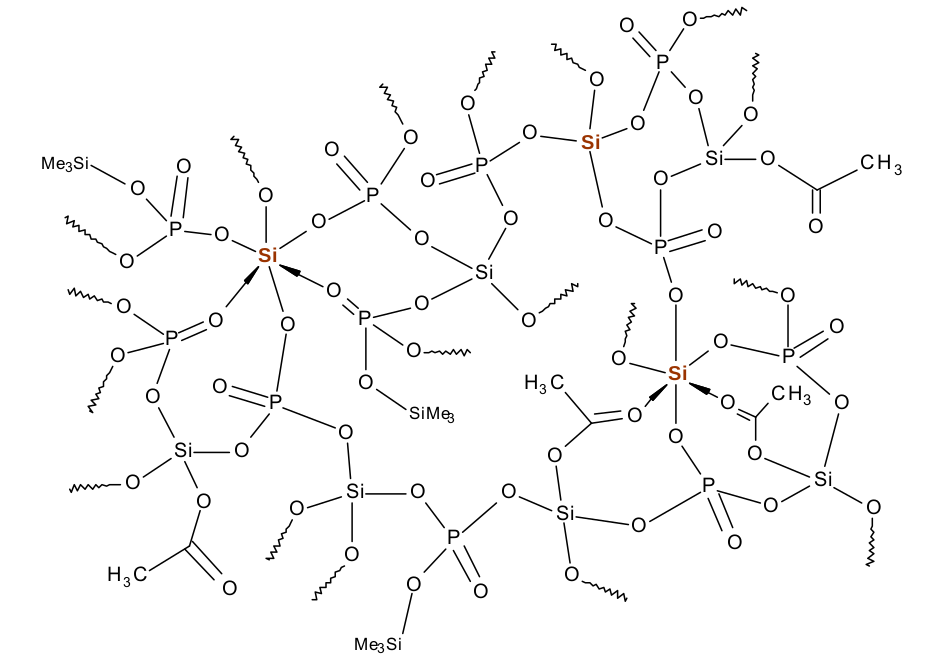
\includegraphics[width=10cm]{si_polymer_cely.png}
  \label{si_polymer_cely}
  \end{figure}


\begin{figure}
\centering
\begin{minipage}{.45\linewidth}
  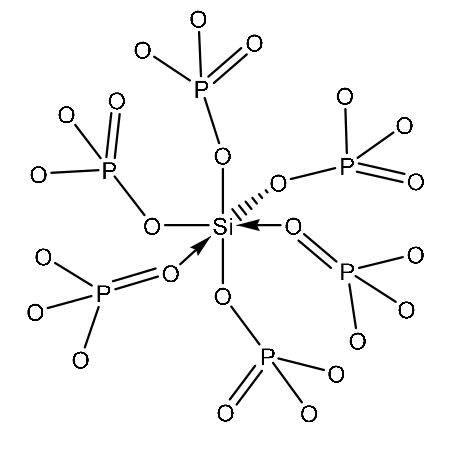
\includegraphics[width=\linewidth]{si_koordinovane_6_P.png}
  \caption{Prostředí kolem Si. \cite{Styskalik2015thesis}}
  \label{img1}
\end{minipage}
\hspace{.05\linewidth}
\begin{minipage}{.45\linewidth}
  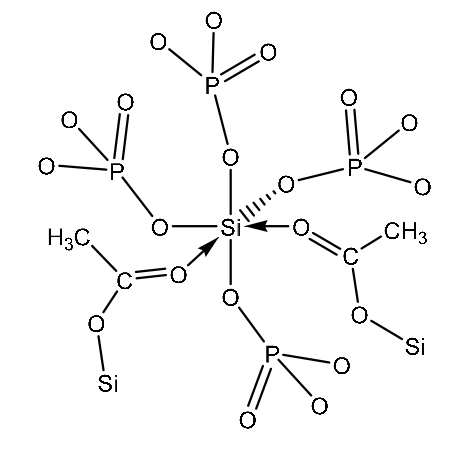
\includegraphics[width=\linewidth]{si_koordinovany_6_C.png}
  \caption{Prostředí kolem Si. \cite{Styskalik2015thesis}}
  \label{img2}
\end{minipage}
\end{figure}

\iffalse
\begin{figure}[h!]
\caption{Prostředí kolem Si. \cite{Styskalik2015thesis} }
  \center
  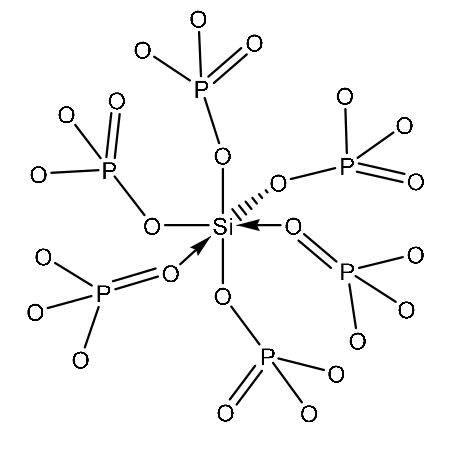
\includegraphics[width=10cm]{si_koordinovane_6_P.png}
  \label{si_koordinovane_6_P}
  \end{figure}
  
  \begin{figure}[h!]
\caption{Prostředí kolem Si. \cite{Styskalik2015thesis} }
  \center
  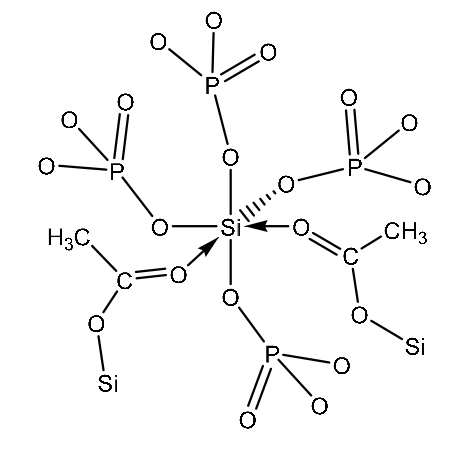
\includegraphics[width=10cm]{si_koordinovany_6_C.png}
  \label{si_koordinovany_6_C}
  \end{figure}
  \fi
\end{otherlanguage}



\chapter{Teoretická část}
Porozumění chemické vazbě mezi atomy daného systému je předpokladem pro vyčerpávající interpretaci získaných experimentálních dat. Na základě znalosti elektronové struktury je často možné také předpovědět spektroskopické vlastnosti a reaktivitu dané molekuly. Pojem chemické vazby je založen na pojmu atom. Počátky tzv. atomové teorie datujeme do období $430-310$ př. n. l. Autorem atomové hypotézy byl řecký filozof Démokritos, který předpokládal, že hmota je stvořena z malých, dále nedělitelných částí. Tato myšlenka byla v pozdějším období alchymie potlačena. Renesance atomové teorie se datuje až do 18.století. John Dalton použil atomovou teorii k popsání průběhu chemických reakcí. Zároveň formuloval zákon stálých poměr slučovacích a zákon stálých poměrů násobných. Od poloviny 19.století se objevují první myšlenky pojmu valence prvků. Německému chemikovi F. A. Kekulému je přisuzováno prvenství předpokladu o čtyřvaznosti uhlíku. Samotné porozumění pojmu valence však bylo možné až po objevení elektronu v roce 1897 J. J. Thomsonem. Toto období může být označeno jako předkvantové období. V roce 1905 bylo publikováno vysvětlení záření černého tělesa, což odstartovalo kvantový popis atomů a molekul.Lewis jako první nahlížel na chemickou vazbu jako na párování elektronů. \cite{Munzarova1996thesis} \\
Kvantový popis atomů a molekul lze obecně rozdělit na lokalizovaný a delokalizovaný. Myšlenka lokalizovaného popisu elektronů ve vazbě je starší a odpovídá představě, že mezi dvěma jádry existuje přímá spojnice, pružina. Autorem popisu chemické vazby s pomocí valenčních vazeb (Valence Bond Theory, VB) je Heitler a London. VB navazuje na myšlenku sdílení elektronových páru od Lewise. Ústřední myšlenkou jsou vazebné orbitaly, kdy největší elektronová hustota je na spojnici dvou jader sousedních atomů. Spojením dvou atomových orbitalů vzniká vazebný orbital. Tomuto popisu se vymyká například uhlík, proto byl vymyšlen koncept hybridizace. Hlavní myšlenkou je, že dojde k spojení orbitalů, které jsou si blízké v energii. Vzniknou tak rovnocenné hybridní orbitaly. \cite{Munzarova1996thesis} \\
Současně s VB se objevovala teorie molekulových orbitalů (Molecular orbital, MO). Elektronová hustota je delokalizována přes všechny atomy a představa chemické vazby jako pružinky neexistuje.\cite{Munzarova1996thesis} \\
Opuštění VB jako popisu chemické vazby bylo zpočátku dáno především vyšší výpočetní náročnosti VB, dále se ukázaly také kvantitativní nedostatky při popisu složitějších molekul. \cite{lowe2011quantum} 

\section{Vlnová funkce a Schrödingerova rovnice}
Chemické vlastnosti molekul určuje jejich geometrická a elektronová struktura. Ve 20. století již bylo známo, že elektrony se svým chováním vymykají představám klasické mechaniky. Na počátku 20. století bylo popsáno chování černého tělesa, fotoelektrického jevu a atomová spektra. Myšlenka, že svět je tvořen z diskrétních částí, kvant, vedla k vzniku kvantové mechaniky. Zlomovou myšlenkou bylo teoretické popsání záření černého tělesa, které vysvětlit Max Planck \ref{eq_Plack}. Předpokládal, že energie se nepředává spojitě ale po přesně daných částech. Na tomto základě Albert Einstein vysvětlil podstatu fotoelektrického jevu, kdy předpokládal, že světlo je složeno z částí a ty nazval fotony. Elektromagnetické vlnění začalo mít částicovou povahu.
\begin{equation}
E = h \nu
\label{eq_Plack}
\end{equation}
$E$ je energie, $h$  je Planckova konstanta\footnote{6, 626 070 040  $\cdot 10^{-34} ~ J \cdot s$ \href{http://physics.nist.gov/cgi-bin/cuu/Value?h}{ Physical Measurement Laboratory of NIST}  }, $\nu$ je frekvence. Na tuto představu navázal Louis de Broglie a navrhl, když vlny mohou mít vlastnosti částic, mohou mít částice vlnové vlastnosti a navrhl rovnici vlny \ref{rce_rovnice_vlny}.
\begin{equation}
\lambda = \frac{h}{mv}
\label{rce_rovnice_vlny}
\end{equation}
$\lambda$ je vlnová délka, $m$ je hmotnosti částice a $v$ je rychlost částice. Částice a vlny mají podle rovnic \ref{rce_rovnice_vlny} a \ref{eq_Plack} duální charakter. Navazující práce se týkala objasnění atomových čárových spekter, kdy atom poskytoval vždy čárová a dokonale reprodukovatelná spektra. I zde byly pomocí myšlenky kvantování později objeveny čáry i mimo viditelnou oblast. Na tyto práce později navázal E. Schrödinger, W. Heisenberg nebo P. A. M. Dirac. a kvantová teorie se začala rozvíjet. \cite{celyprincipy}\\
V běžné mechanice je systém možné přesně popsat polohou a hybnosti, díky těmto veličinám lze předvídat i pohyb budoucí. V kvantové mechanice je veškerá interpretace pravděpodobnostní. Vždy lze říci, že se daná částice bude v nějakém prostoru v daném čase vyskytovat pouze s určitou pravděpodobností. Informaci o částici v sobě nese Schrödingerova rovnice \ref{SCH_time_dependent}, diferenciální rovnice druhého řádu.\cite{polak2000obecna}
\begin{equation}
i \hbar \frac{\delta}{\delta t} \Psi (\vec{r},t)=\widehat{H} \Psi(\vec{r},t)
\label{SCH_time_dependent}
\end{equation}
$\widehat{H}$ je Hamiltonián, operátor, který reprezentuje kvantově mechanickou cestu k výpočtu energie systému, $E$ je energie, vlastní hodnota Hamiltoniánu, $\Psi$ je vlnová funkce, která v sobě ukrývá celou informaci o systému, $\hbar$ je redukovaná Planckova konstanta. Hamiltonián se skládá ze dvou částí, operátoru kinetické a potenciální energie.
\begin{equation}
\widehat{H} = \widehat{T} + \widehat{V}
\end{equation}
$\widehat{T}$ reprezentuje kinetickou enregii, $\widehat{V}$ je potenciální energie. Kvantově mechanický výraz pro kinetickou energii $\widehat{T}$ je sumou jednočásticových operátorů. 
\begin{equation}
\widehat{T_i} = - \frac{h^2}{8 \pi ^2} \sum \frac{1}{m_i} \left( \frac{\delta^2}{\delta x_i^2} +\frac{\delta^2}{\delta y_i^2} +\frac{\delta^2}{\delta z_i^2} \right)
\end{equation}
$m_i$ je hmotnost $i-té$ částice. Kvantově mechanický výraz pro potenciální energii $\widehat{V}$ je coulombovská interakce mezi částicemi.
\begin{equation}
\widehat{V} = \sum_{i<j}\sum \left( \frac{e_i e_j}{r_{i,j}}\right)
\end{equation}
 Pro účely této práce postačí stacionární Schrödingerova rovnice, která v sobě nezahrnuje čas \ref{schrodingerova_rovnice}.\\
 \begin{equation}
\widehat{H}\Psi = E \Psi
\label{schrodingerova_rovnice}
\end{equation}
Vlnovou funkci $\Psi$ lze získat řešením Schrödingerovy rovnice \ref{schrodingerova_rovnice}. Fyzikální význam má pouze $|\Psi|^2$, což vyjadřuje hustotu pravděpodobnosti výskytu elektronu. Tento matematický prostor se nazývá orbital. Exaktní řešení \ref{schrodingerova_rovnice} existuje pouze pro atom vodíku a další exotické atomy, které mají jeden elektron a jeden proton. Při rozšíření atomu byť i jeden elektron se \ref{schrodingerova_rovnice} stává analyticky neřešitelnou. Na řádu přichází numerické přístupy a aproximace. Pro atom s více elektrony lze k problému přistoupit tak, že elektrony nebudou vzájemně interagovat. Toto řešení pro chemii prakticky nemá význam, lze s tím řešit pouze speciální případy iontů. Hartree přišel na způsob řešení, kdy se elektron pohybuje časové průměrném poli ostatních jader. \cite{warren1986ab}
Příslušnou vlnovou funkci pro atom s více elektrony \ref{eq_MO} lze zapsat součin jednoelektronových funkcí \ref{eq_AO}.  V základu je navrhnuta hrubá vlnová funkce, která poskytuje energii vyšší než je energie základního stavu. Tato funkce \ref{eq_MO} je variačním přístupem upravována, dokud není nalezena nejnižší energie.  
\begin{equation}
\psi_{AO} = 1s(1)
\label{eq_AO}
\end{equation}
\begin{equation}
\psi_{MO} = 1s(1) \cdot 2s(1)
\label{eq_MO}
\end{equation} 
Zároveň musí platit, že všechny orbitaly musí být vzájemně orthogonální a normalizované.
\begin{equation}
S_{ii} = \int \psi_i * \psi_i dx dy dz = 1 ~ \bigwedge ~ S_{ij} = \int \psi_i * \psi_j dx dy dz = 0
\end{equation}
V tomto přístupu jsou ovšem není dodržena antisymetrii vlnové funkce (Pauliho princip). \cite{warren1986ab}
\begin{equation}
\Psi (1,2) = - \Psi (2,1)
\label{Paulliho_princip}
\end{equation}
 Každá jednoelektronová funkce má prostorou a spinovou část, tzv.~spinoorbital. Pro mnohaelektronové atomy už je pro správný výpočet energie vzít spin v úvahu.  Antisymetrii a spin do Hartreeho metody zavedl Vladimir Aleksandrovič Fock a John Slater. Výsledkem byla Hartree-Fockova metoda self-konzistentního pole(HF-SCF), kde se funkce s nejnižší energii hledá iterativním způsobem za pomoc variačního počtu. Vlnová funkce se zapisuje pomocí Slaterova determinantu, SD, který má obecný tvar \ref{Slateruv_determinant}. SD zaručuje antisymetrii vlnové funkce vůči výměně polohových a spinových souřadnic. $\psi_i$ je jednoelektronová vlnová funkce, $s_j$ jsou elektrony, $\sqrt{N!}$ je normalizační faktor.
\begin{equation}
\psi =  \frac{1}{\sqrt{N!}}\begin{vmatrix}
\psi_1(1)\alpha(1) & \psi_1(1) \beta (1) & \psi_2(1)\alpha(1) & \dots & \psi_{n/2}(1)\beta(1) \\
\psi_1(2)\alpha(2) & \psi_1(2) \beta (2) & \psi_2(2)\alpha(2) & \dots & \psi_{n/2}(2)\beta(2) \\
\vdots             & \vdots              & \vdots             & \ddots & \vdots \\
\psi_1(n)\alpha(n) & \psi_1(n) \beta (n) & \psi_2(n)\alpha(n) & \dots & \psi_{n/2}(n)\beta(n) 
\end{vmatrix}
\label{Slateruv_determinant}
\end{equation}
U atomů s více  elektrony chemie začíná, hlavním cílem je získat znalosti o molekulách. V tomto systému se nově objevuje více než jedno jádro a systém se stává opět příliš složitý pro matematické řešení. Ve skutečnosti je proton přibližně $1800 \times$ těžší než elektron, tudíž je rychlost mnohem menší, než rychlost elektronu. Situace lze zjednodušit oddělením pohybu elektronů od pohybu jader a řešit tak problémy odděleně. Přístup byl navržen jako Born$-$Oppenheimerova aproximace \ref{eq_B_O_aproximace}. Vlnová funkce elektronů závisí pouze na poloze jader, ne jejich rychlosti.\cite{lechamolecularmodeling} Zároveň je vlnová funkce parametricky závislá na poloze jader, pro každou geometrii jader je získána jiná vlnová funkce. Závislost energie na poloze jader se pro víceatomové molekuly nazývá hyperplocha potenciální energie. \cite{dftshrnutivysledky}
\begin{equation}
\Psi_{tot}(nuclei, elektrons) = \Psi(electrons) \cdot \Psi(nuclei)
\label{eq_B_O_aproximace} 
\end{equation}

\section{Metody kvantové chemie}
Metody výpočetní chemie lze ve stručnosti shrnutou na \textit{Ab inito} metody, semi-empirické metody a DFT metody. \textit{Ab inito} metody řeší Schröfingerovu rovnici bez použití parametrů z experimentálních dat.  Vzájemnou souvislost a podobnost metody vystihuje schéma na obrázku \ref{schema_QM}.
 \begin{figure}[h]
\caption{Schéma post-Hartree-Fockových teorií, $n^m$ je škálování vzhledem k velikosti systémy \cite{pdf_obrazek}. }
  \center
  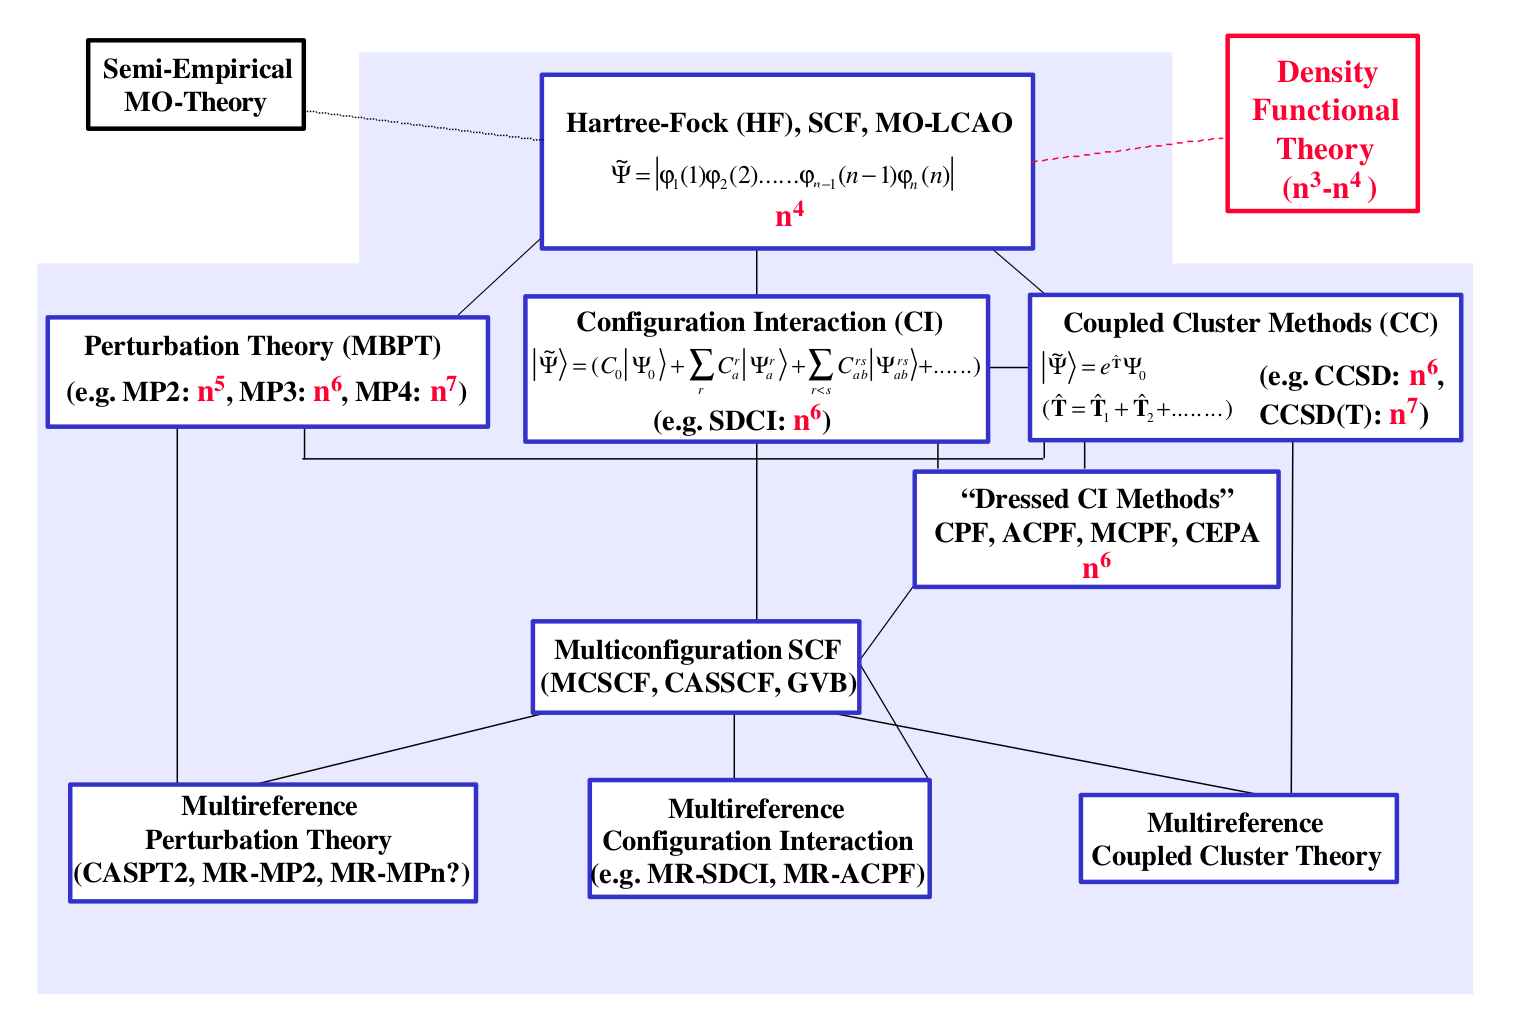
\includegraphics[width=12cm]{schema_QM.png}
  \label{schema_QM}
  \end{figure}
  Metody QM vychází z řešení stacionární Schrödingerovy rovnice \ref{schrodingerova_rovnice}. Semiempirické metody řeší Schrödingerovu rovnici pouze částečně, některé parametry jsou dodány z experimentů. \\
     Základní aproximací je Born-Oppenheimerova aproximace a zapsání vlnové funkce jako Slaterův determinant pomocí atomových orbitalů. Z tohoto základu vznikla Hartree, která navíc uvažuje elektron v průměrném poli zbylých elektronů. Zde pomocí variačního přístupu hledá nejvhodnější energii. Antysymetrii vlnové funkce zajistí SD a Fockovy rovnice, proto Hartee-Fockova metoda. Samotný HF přístup v sobě neobsahuje korelaci pohybu elektronů. Tento faktor je tam možno vložit dodatečně pomocí tradičních \textit{ab inito} metod Many-Body Pertrubation  theory (MBPT), konfigurační interakcce (configuration interaction, CI) nebo spřažené klastry( coupled cluster methods, CC). Śkálování těchto metod je uvedeno na obrázku \ref{schema_QM}. Tyto metody jsou přesné, ale výpočetně velice náročné proto nejsou vhodné pro příliš velké systémy. Řešením je použití teorie funkcionálu hustoty (The Density Functional theory, DFT) nebo Rozšířenou Hückelovu metodu (The Extenden Hückle theory, EHT).

\section{Rozšířená Hückelova metoda}
EHT se řadí mezi semiemprické metody, které  pro výpočet energie používají klasický \textit{ab inito} přístup, pouze jsou některé parametry vzaty z experimentu. Tím se snižuje výpočetní náročnost. Přes její jednoduchost dává dobré kvalitativní výsledky především v oblasti molekulových orbitalů. EHT navazuje na Hückelův přístup, který platil pro konjugované systémy. EHT může být použita i pro systémy se $\sigma$ vazbami. Na rozvoji teorie se podílel Roald Hoffman. \cite{lowe2011quantum} \\
Základem metody je sekulární rovnice, která je známá již z metody MO-LCAO. (viz. sekulární rovnice v metody MO-LCAO). EHT poskytuje jednoduché řešení členu $H_{ij}$ pomocí vzorce \ref{EHT_vypocet_H} a empirických parametrů. $S_{ij}$ je překryvový integrál, $E$ je hlednanní energie.
\begin{equation}
E = \begin{vmatrix}
H_{11} - E S_{11} & H_{12} - E S_{12} & \dots & H_{1j} - E S_{1j} \\
H_{21} - E S_{21} & H_{12} - E S_{22} & \dots & H_{1j} - E S_{2j} \\
\vdots & \vdots &  \ddots & \vdots  \\
H_{i1} - E S_{i1} & H_{i2} - E S_{i2} & \dots & H_{ij} - E S_{ij} \\
\end{vmatrix}
\end{equation}


\begin{equation}
H_{ij} = K S_{ij} \left( \frac{H_{ii} + H_{jj}}{2} \right)
\label{EHT_vypocet_H}
\end{equation}
kde $K$ si parametr, jehož hodnota byla R. Hoffmannnem stanoevna na 1,75. 

\section{Metoda funkcionálu hustoty}
DFT metody jsou založeny na vztahu mezi elektronovou hustotou a celkovou energii systému, teorie funkcionální \footnote{Funkcionál je operátor, který zobrazuje z prostoru funkcí do množiny obecně komplexních čísel} hustoty. Elektronová hustota $\varrho(\pmb{r})$ je pravděpodobnosti, že v nějakém bodě prostoru nalezneme nějaký elektron.  Výhodou tohoto přístupu je, že elektronová hustota je funkcí pouze tří prostorových souřadnic. Tento výpočetní model byl objeven už v roce 1920, pro chemii začal mít význam až v 60. letech 20. století. Výpočetně podobně náročná jako HF, ale přesnější, obsahují korelační energii. \\

V roce 1964 uveřejnili Koch a Hohenberg dva teorémy, které ukázaly, že energie základního stavu  a další vlastnosti jsou jednoznačně určeny elektronovou hustotou. Energie je funkcionál elektronové hustoty .
\cite{lechamolecularmodeling}
\subsection{Principy}
\subsubsection{První Hohenberg- Kohn teorém}
Pro libovolný systém interagujících elektronů je externí potenciál $V_{ext}$ jednoznačně
určen elektronovou hustotou (až na konstantu). \cite{dftshrnutivysledky}
\begin{equation}
E_{el} = E_{el} (\varrho)
\end{equation}
 Za znalosti elektronové hustoty lze vypočítat energii a všechny ostatní vlastnosti základního stavu.
\subsubsection{Druhý Hohenberg-Kohn teorém}
Druhý teorém je postaven na variačním principu. Poskytuje informace, jak lze najít elektronovou hustotu, která poskytne nejnižší a zároveň nejpřesnější energii.
\cite{koch2000chemist} 
Předpokládejme, že danému externímu potenciálu $V'_{ext}$ přísluší elektronová hustota
$\varrho_0$. Pak pro jakoukoli jinou elektronovou hustotu $\varrho_0$ bude platit
\begin{equation}
E [\varrho_0] < E[\varrho ']
\end{equation}

\subsubsection{Kohn-Shamovy rovnice}
Při hledání vhodného funkcionálu je zásadní problém zahrnout kinetickou energii elektronů, klasickou coulombickou interakci mezi elektrony a dále korelační a výměnné efekty. Hlavní myšlenkou bylo rozdělení hledaného funkcionálu $F(\varrho(\vec{r}))$ do menší částí. \cite{koch2000chemist}
\begin{equation}
F(\varrho(\vec{r})) = T_s[\varrho(\vec{r})] + J[\varrho(\vec{r})] + E_{EX}[\varrho(\vec{r})]
\end{equation}
 Kinetickou energii $T_s$ lze započítat jako Shamův potenciál. Lze sestavit pole neinteragujících elektronů, které bude mít stejnou elektronovou hustotu jako reálný systém interagujících elektronů. $T_{s}$ lze počítat jako součet jednoelektronových funkcí \ref{kineticka_energie_jednoelektronova}. \cite{koch2000chemist}
\begin{equation}
T_s = -\frac{1}{2} \sum_{i=1} ^{N}  \bra{\psi_i}{\nabla^{2}}\ket{\psi_i}
\label{kineticka_energie_jednoelektronova}
\end{equation}
Tímto způsobem vypočítaná $E_{kin}$ není skutečná $E_{kin}$ systému. \\
$J[\varrho(\vec{r})]$ je 
\subsection{DFT v praxi}
Výběr vhodného funkcionálu je nelehký úkol. Funkcionály mohou být obecně rozděleny na tři kategorie. Aproximace lokální hustoty (Local Density Approximation, LDA), metoda zoběcněného gradientu (Generalized Gradient Approximation, GGA) a poté hybridní funkcionály. \cite{dftshrnutivysledky}
\subsubsection{Aproximacce lokální hustoty}
LDA funkcionály vychází z modelu homogenního elektronového plynu, kdy máme v celém systému konstantní elektronovou hustotu.\cite{dftshrnutivysledky} V základu se jedná o \textit{ab inito} přístup, přesto má pro chemii využití pouze pro valenční elektrony. Často totiž v molekulách není pravidelná distribuce elektronové hustoty. Prostor lze rozdělit na jednotky objemu a elektronovou hustotu sčítat přes objem podle rovnice.
\begin{equation}
E_{XC}^{LDA} = \int \varrho (\vec{r} \epsilon_{XC} (\varrho (\vec{R})) d \vec{r}
\label{LDA_vyraz_pro_obecnou_energii}
\end{equation}
Tvar $\epsilon_{XC}(\varrho (\vec{r}))$je výměnně-korelační energie pro jeden elektron, která může být rozdělena na výměnnou a korelační část. 
\begin{equation}
\epsilon_{XC}(\varrho (\vec{r})) = \epsilon_x (\varrho) + \epsilon_c (\varrho)
\label{LDA_tvar_vymene_korelacni_energie}
\end{equation}
Výměnný člen lze zapsat analyticky, známy pod názvem Slaterův výměnný člen, značen S.
\begin{equation}
\epsilon_{XC}(\varrho (\vec{r})) = - \frac{3}{4} \sqrt[3]{\frac{3 \varrho (\vec{r})}{\pi}}
\label{LDA_vymenny_clen}
\end{equation}
Korelační energii lze zavést metodou VWN (auto rVosko, Wilky a Nuisar) pomocí numerických výpočtů. Vylepšením je spinově závislá aproximace lokální hustoty, která zavádí elektrony se spinem $\alpha$ a $\beta$.
\begin{equation}
E_{XC}^{LSD}[\varrho_{\alpha}, \varrho_{\beta}] = \int \varrho (\vec{r} \epsilon_{XC}( \varrho_{\alpha}(\vec{r}), \varrho_{\beta}(\vec{r})) d \vec{r}
\end{equation}
\cite{koch2000chemist}
\subsubsection{Metoda zobecněného gradientu}
GGA funkcionál vychází z aproximace lokální hustoty, která je dále vylepšována. Jedna z možností je použít \textbf{gradient elektronové hustoty} $\nabla \varrho (\vec{r})$.  \cite{koch2000chemist}

\subsubsection{Hybridní funkcionály}
Přístup kombinuje HF vzorec pro výpočet energie ( \textbf{dát odkaz}) a výměnné funkcionály. 
Do této kategorie patří nejznámější funkcionál \textbf{B3LYP}.
\begin{equation}
E_{ex}^{B3LYP} = (1-a_0-a_x)E_x^{LDA} + a_0E_x^{exact} + a_x^{B88} + (1-a_c)E_c^{VWN} + a_c^{LYP}
\label{B3LYP_rovnice}
\end{equation}
$a_0$, $a_x$ a $a_c$ jsou nastavitelné parametry. \textbf{B3LYP} má 20\% podíl výměnné energie. \cite{dftshrnutivysledky}




Předchůdci Aproximace lokální hustoty LDA a GGA funkcionály. B3LYP \footnote{vyvinut v roce 1993} je hybridní funkcionál, který vznikl jako kombinace BLYP (GGA) a výpočtu z Kohn-Slamových orbitalů(vypočítáme část výměnné energie).


\section{Báze v \textit{ab inito} výpočtech }\label{kapitola_baze}
Množina funkcí, ze kterých jsou skládány orbitaly, se nazývá bazí atomových orbitalů. Pro výběr funkcí platí dvě základní pravidla. Příslušné bázové funkce musí dostatečně dobře popsat vlnovou funkci, aby získané výsledky měly chemický význam. Zároveň integrály $F_{ij}$ a $S_{ij}$ musí být řešitelné v rozumně dlouhém časem. \cite{lowe2011quantum}
Pro popis atomu lze použít minimální nebo rozšířené báze. Minimální báze obsahuje pouze funkce, které popisují orbitaly obsazené v základním stavu daného atomu. Rozšířená báze obsahuje například polarizační funkce nebo difuzní funkce. Mezi základní typy bazí pro atomové orbitaly jsou orbitaly vodíkové typu, orbitaly Slaterova typu (STOs) a gaussovské funkce. \cite{dftshrnutivysledky}
Orbitaly vodíkového typu mají radiální a angulární část. Orbitaly vodíkového mají nevýhodu ve své složitosti a často je nutné použít numerické řešení problému. STO orbitaly nemají radiální uzly a pro některé integrály neexistuje analytické řešení. STO orbitaly jsou ve tvaru polynomu souřadnic a exponenciály\ref{STO_orbital}.\cite{jensen2007introduction}
\begin{equation}
\chi_{\zeta, n, l, m}(r, \theta, \varphi) = NY_{l,m} (\theta, \varphi) r^{n-1} e^{-\zeta r}
\label{STO_orbital} 
\end{equation}
$N$ jr normalizační faktor, $Y_{l,m}$ sféricky harmonická funkce, exponent závisí na vzdálenosti od jádra. Radiální část je tvořena jako lineární kombinace STO. Především přidáváním bázových funkcí STO typu enormně narůstá výpočetní čas. Alternativou jsou Gaussovské orbitaly (Gausian type orbitals, GTO).
\begin{equation}
\chi(r) = Nr^n e^{-a(r-r_A)^2}
\end{equation}
 Výhodou GTO je to, že jejich součin je stále GTO a hledání $F_{ij}$je výpočetně nenáročné. Na rozdíl od ostatních funkcí nemají správné chování na jádře. Z tohoto důvodu je báze STO orbitalů tvořena několika GTO, které jsou označovány jako primitivní Gaussovské funkce.Největší přínos GTO je rozdíl v druhé mocnině vzdálenosti v exponenciálním členu.\cite{lowe2011quantum}. 
 V současné době existuje obrovské množství bazí, které lépe či hůře popisuje zvolený problém. Mezi základní báze jsou uváděny DZP, STO-3G a různé druhy 6-31G. DZP je double-zeta gassovská báze s polarizací, STO-3G jsou Slaterovy orbitaly zjednodušeny jako lineární kombinace tří primitivních gaussiánů, odpovídá minimální bázi. 3-21G jsou označovány jako \uv{split valence basics sets}. Vnitřní elektrony jsou popisovány tří primitivními gaussiány, valenční orbitaly  do dvou primitivních gaussiánů a jednoho jednoduchého gaussiánu. Pro bázi 6-31G je vnitřní oblast tvořena šesti primitivními gaussiány, ostatní je obdobné jako pro 3-21G. Báze 6-21*G je v základu obdobná, * označuje polarizační funkci. Přidává p orbital pro vodíky a d orbitaly pro těžší atomy. Symbol ** označuje přidání d orbitalů pro vodík.(zdroj je 3 pdf soubory z hodiny Metody kvantové chemie). \\
 DFT metodou lze krom optimalizací počítat také parametry nukleární magneetické rezonance (NMR). Jedním z NMR charakteristik molekul je chemické stínění. Do \textit{ab-inito} výpočtu nově vstupuje vnější magnetické pole $B_0$, které je reprezentováno vektorovým potenciálem tohoto pole. V ideálním případě by neměla mít volba počátku tohoto pole vliv na výsledek. Jedním z důsledků aproximace v kvantové chemii je fakt, že volba počátku výrazně ovlivňuje výsledné chemické stínění. Problém se nazývá \uv{Gauge origin problem}. Metoda IGLO (Individual Gauge for Localization Orbitals)řeší problém způsobem, že zahrnují počátek vektorového potenciálu do atomových orbitalů nebo do lokalizovaných molekulových orbitalů.\cite{Standara2006thesis}

\subsection{Kvalitativní koncepty v kvantové chemii}
Důležitou součástí výzkumu v oblasti kvantové chemie jsou zjednodušené koncepty, které pomáhají s interpretací kvantově$-$chemických dat. Jedním z příkladů je vysvětlení vaznosti atomů a molekul. \\
Lewisovská teorie chemické vazby nahlíží na vazbu jako na lokalizovaný koncept, kde jsou elektrony na spojnici jader. Tento jednoduchý koncept předpokládá, že platí tzv. oktetové pravidlo a maximální počet vazeb odpovídá číslu skupiny, ve které se atom nachází. Tato teorie si bohužel nedokáže poradit už s molekulou methanu. Podle Lewisovské teorie by měl uhlík tvořit dvojvazné molekuly. V případě čtyřvazných molekul by měly být dvě vazby rovnocenné a dvě o nižší energii kvůlu zapojení rozdílných orbitalů. V methanu ale najdeme čtyři stejně dlouhé a naprosto rovnocenné vazby. Vysvětlení této skutečnosti nabízí teorie hybridizace. Ta předpokládá, že může dojít ke sjednocení orbitalů o blízké energii, za vzniku hybridního orbitalu. Tímto způsob vytvořené vazby si jsou naprosto rovnocenné. Ani koncept hybridizace nevysvětluje všechny případy vaznosti molekul. Pro některé atomy jsou si orbitaly natolik vzdálené, že hybridizace nepřichází v úvahu. Nejlepším popisem pro tyto systémy jsou molekulové orbitaly. Ty zavádí do celého popisu princip delokalizace. Mezi molekuly, které se vymykají Lewisovskému přístpupu, lze zařadit obecně sloučeniny vzácných plynů (fluoridy xenonu),  \ce{SF6}, \ce{ClF3} a \ce{I3^-}. \\

Ochotu tvořit hypervalentní molekuly lze odhadnout podle konceptu HSAB (Hard and Sfot Acids and Basics). Kyseliny a báze mohou být rozděleny na měkké a tvrdé. HSAB teorie říká, že tvrdá kyselina a tvrdá báze spolu poskytnou stabilní komplex, naopak slabá kyselina a slabá báze spolu poskytnou méně stabilní komplex. Z toho vyplývá, že ze znalosti reakčních podmínek a příslušné tvrdosti lze predikovat stabilitu vzniklého komplexu. Jeden z možností kvantitativního určení tvrdosti/měkkosti je určení parametrů $\chi$ \footnote{Elektronegativity byla Paulingem definována pomocí ionizačního potenciálu a elektronové afinity} \ref{hsab_vypocet_elektronegativita} a $\eta$ \ref{hsab_vypocet_tvrdost}. \cite{hsabclanek}. 
\begin{equation}
\chi = - \left( \frac{\delta E}{\delta N} \right) = \frac{IP + EA}{2} = -\mu
\label{hsab_vypocet_elektronegativita}
\end{equation} 
\begin{equation}
\eta = \frac{1}{2} \left( \frac{\delta \mu}{\delta N} \right) = \frac{1}{2}\left( \frac{\delta^2 E}{\delta N^2} \right) = \frac{I - A}{2}
\label{hsab_vypocet_tvrdost}
\end{equation} 
$\chi$ je elektronegativita, $\chi$ je elektronegativity, $E$ je energie a $N$ je počet elektronů. \cite{hsabwatoc} Podle Koopmansova teorému $E_{HOMO} = - IP$, $IP$ je ionizační potenciál a $E_{LUMO} = EA$, $EA$ je elektronová afinita.\cite{kratochvilexcerpta} $\eta$ je atomová tvrdost \footnote{$\eta = \frac{1}{\sigma}$, $\sigma$ je měkkost atomu}. \cite{hsabwatoc} Tvrdá kyselina a báze je charakterizována velkým rozdílem $IP$ a $IA$, což se projeví jako vysoké hodnoty $\chi$ a $\eta$. Při znalosti $E_{HOMO}$ a $E_{LUMO}$ lze predikovat ochotu reakčního centra interagovat s námi zvoleným reagentem a zároveň odhadnout stabilitu vzniklého komplexu. Systémy s velkým rozdílem $E_{HOMO}$ a $E_{LUMO}$ jsou tvrdší, stabilnější a méně reaktivní.




\chapter{Výpočetní část}
Cílem praktické výpočetní části bylo zkoumat struktury fosfokřemičitanů metodou EHT a DFT. Pro metodu EHT byly vybrány menší struktury, metodou DFT byly zkoumány větší struktury.
\section{Struktury získané metodou EHT}
Pro popis EHT metodou byly zvoleny tři čtyř koordinované sloučeniny křemíku \ce{H4SiO4}, \ce{Si(OH)3CH3} a \ce{Si(OH)3P(OH)2} a jedna šestikoordinovaná sloučenina \ce{H6SiO6}.
%H4SIO4
% --------------------------------------------------------------------------
\subsection{Molekula H$_4$SiO$_4$}
Základní molekula pro čtyřkoordinovaný křemík je \ce{H4SiO4}, kde Si je koordinován čtyřmi kyslíky. Před výpočtem metodou EHT byla struktura optimalizována. \ref{obr_h4sio4_opt_struktura}

\begin{figure}[h!]
\caption{Optimalizovaná struktura \ce{H4SiO4}. }
  \center
  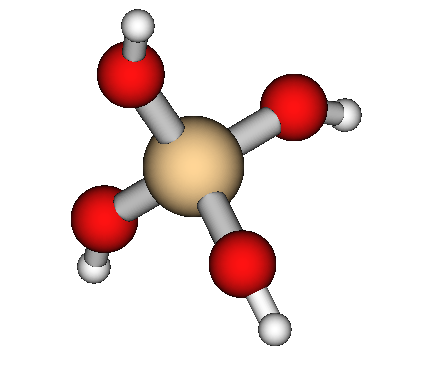
\includegraphics[width=5cm]{h4sio4_obr.png}
  \label{obr_h4sio4_opt_struktura}
  \end{figure}
  
\begin{table}[htbp]
\begin{minipage}{\textwidth}
\caption{Výsledné mísení orbitalů pro \ce{H4SiO4}}
\begin{center}
\begin{tabular}{|r|r|r|r|r|r|}
\hline 
\multicolumn{2}{|c|}{$\bra{20}{\hat{H}}\ket{24}$, $\bra{16}{\hat{H}}\ket{24}$} & \multicolumn{2}{|c|}{$\bra{11}{\hat{H}}\ket{21}$, $\bra{19}{\hat{H}}\ket{21}$}& \multicolumn{2}{|c|}{$\bra{15}{\hat{H}}\ket{22}$, $\bra{18}{\hat{H}}\ket{22}$} \\
\hline \hline
\multicolumn{1}{|l|}{MO\footnote{Molekulový orbital} } & \multicolumn{1}{r|}{W\footnote{součet procentuálních příspěvků příslušných fragmentových orbitalů do příslušného molekulového orbitalu}} & \multicolumn{1}{l|}{MO} & \multicolumn{1}{r|}{W} & MO & \multicolumn{1}{r|}{W} \\ \hline
1 & 84 \% & 4 & 67 \% & 2 & 65 \% \\ \hline
20 & 91 \% & 16 & 79 \% & 19 &  97 \% \\ \hline
24 & 99 \% & 21 & 100 \% &  22& 100 \% \\ \hline
\end{tabular}
\end{center}
\label{tab_h4sio4_vysledky}
\end{minipage}
\end{table}
  %  Pro fragmentové orbitaly $\bra{22}{\hat{H}}\ket{26}$, $\bra{7}{\hat{H}}\ket{26}$ byly nalezeny příslušné molekulové orbitaly \ref{obr_h4sio4_MO_s1_1}, \ref{obr_h4sio4_MO_s1_20} a \ref{obr_h4sio4_MO_s1_24} .
    Fragmentové orbitaly 7, 22 a 26 se navzájem mísí za vzniku MO číslo 1, 20 a 24, znázorněných na obrázku \ref{obr_h4sio4_vysledky_I}.
 %-------------
\begin{figure}
\begin{center}
\subfigure[MO 1]{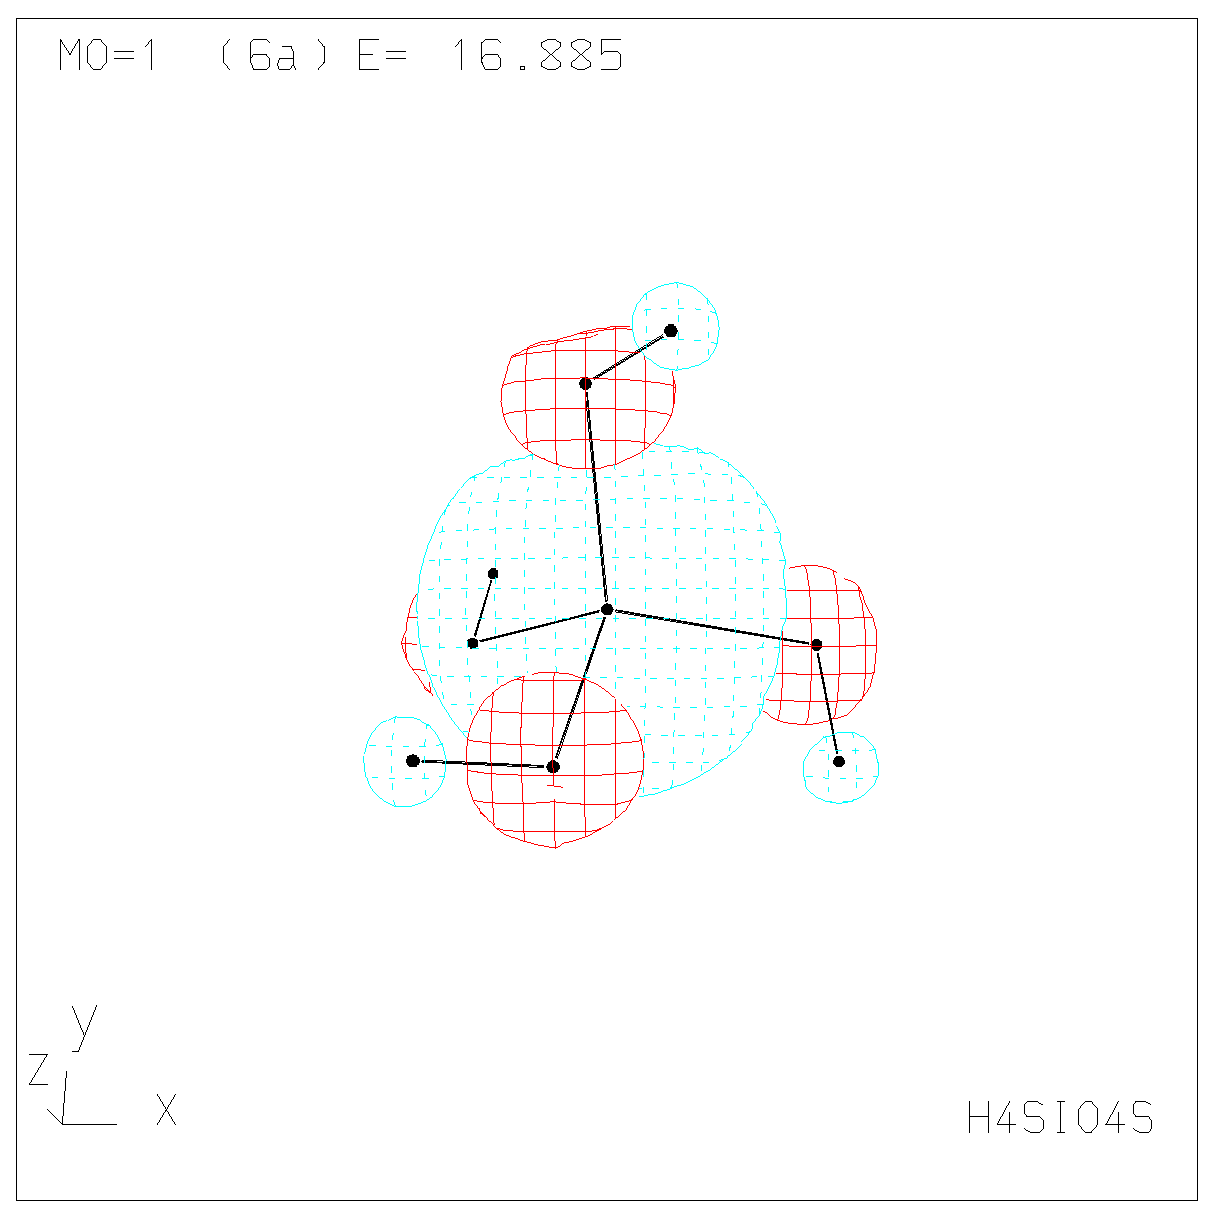
\includegraphics[width=5cm]{h4sio4_obrazky/s1_1.eps} \label{obr_h4sio4_MO_s1_1}}
\subfigure[MO 20]{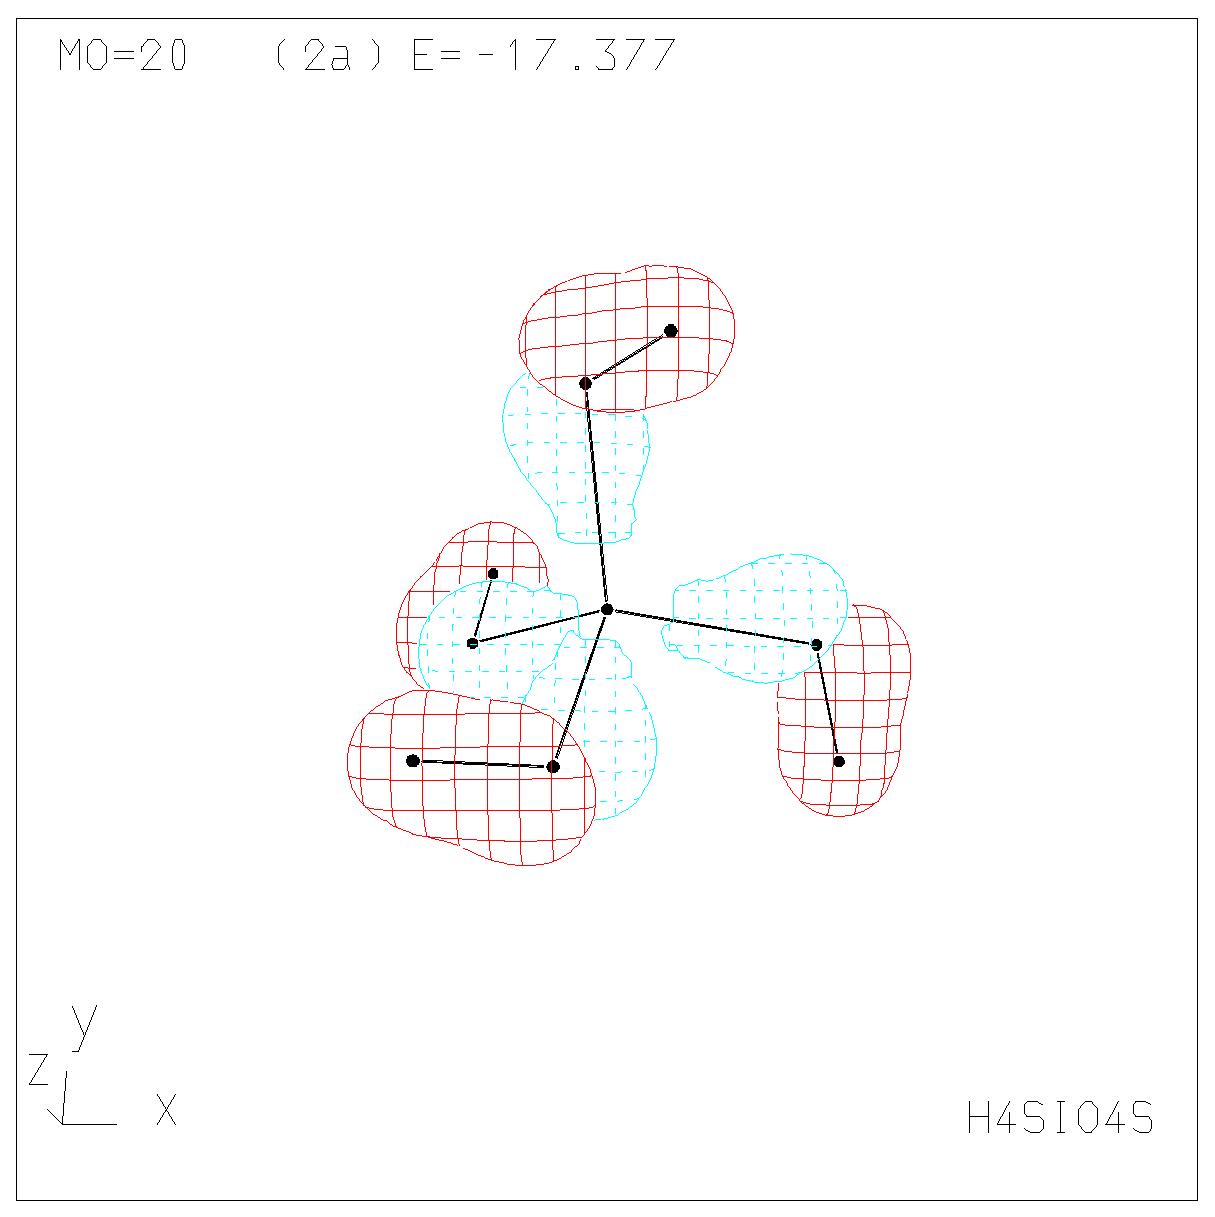
\includegraphics[width=5cm]{h4sio4_obrazky/s1_20.eps}\label{obr_h4sio4_MO_s1_20}}
\subfigure[MO 24]{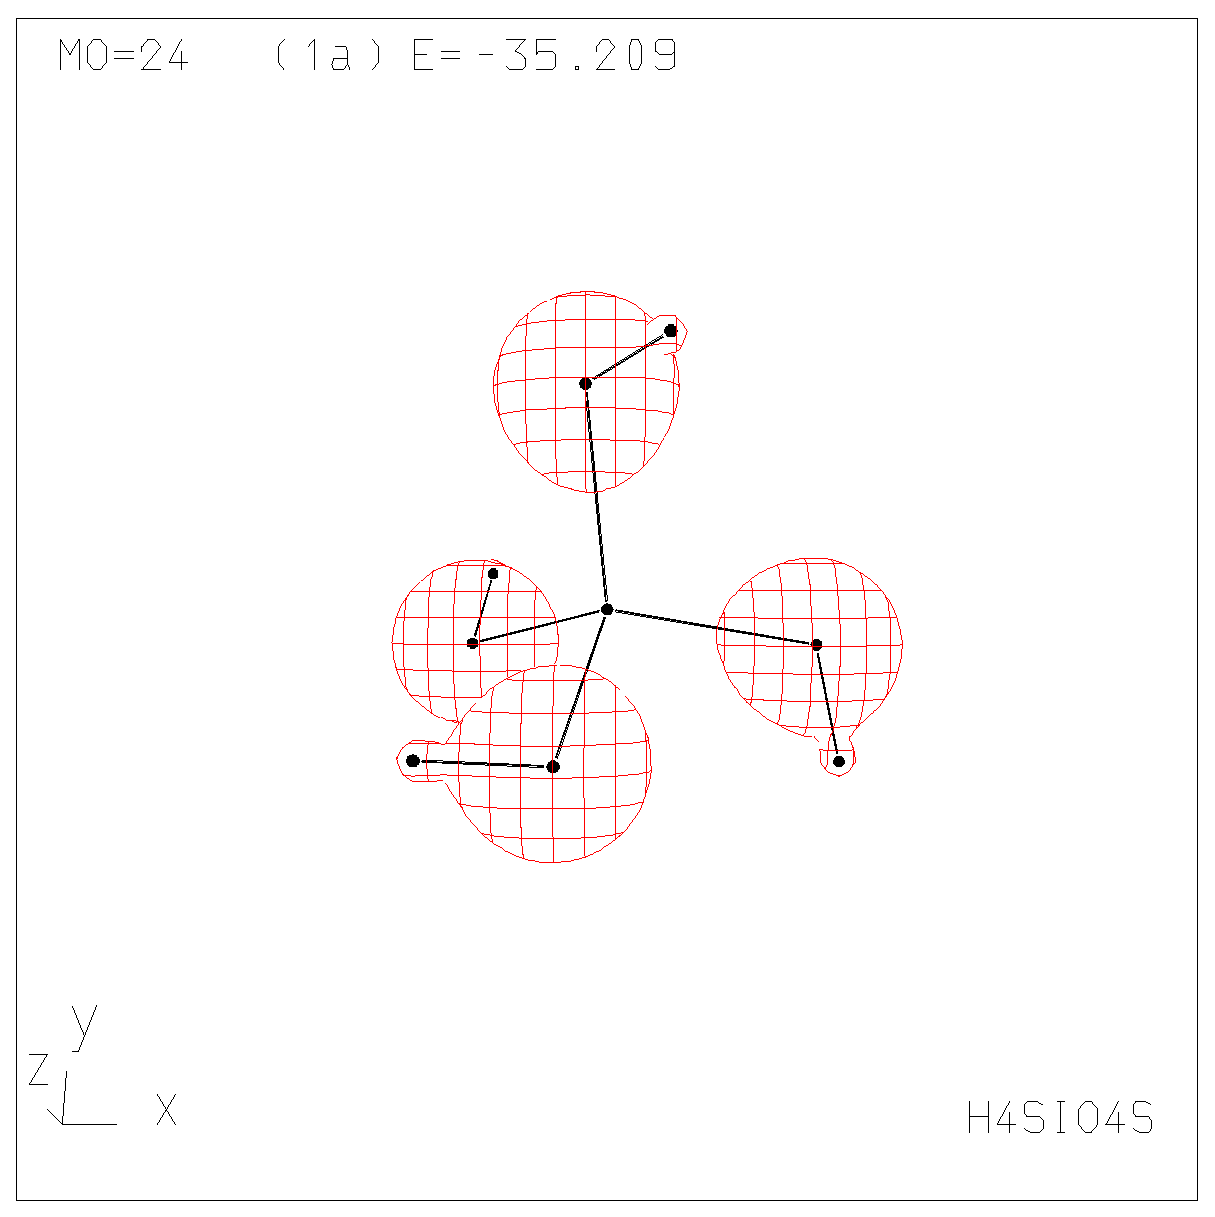
\includegraphics[width=5cm]{h4sio4_obrazky/s1_24.eps}\label{obr_h4sio4_MO_s1_24}}
\caption{Interakce $\bra{22}{\hat{H}}\ket{26}$, $\bra{7}{\hat{H}}\ket{26}$ z tabulky \ref{tab_h4sio4_vysledky}.}

\label{obr_h4sio4_vysledky_I}
\end{center}
\end{figure}


%------------    
Fragmentové orbitaly  11, 19 a 21 se navzájem mísí za vzniku MO číslo 4, 16 a 21, znázorněných na obrázku \ref{obr_h4sio4_vysledky_II}.   
\begin{figure}
\begin{center}
\subfigure[MO 4]{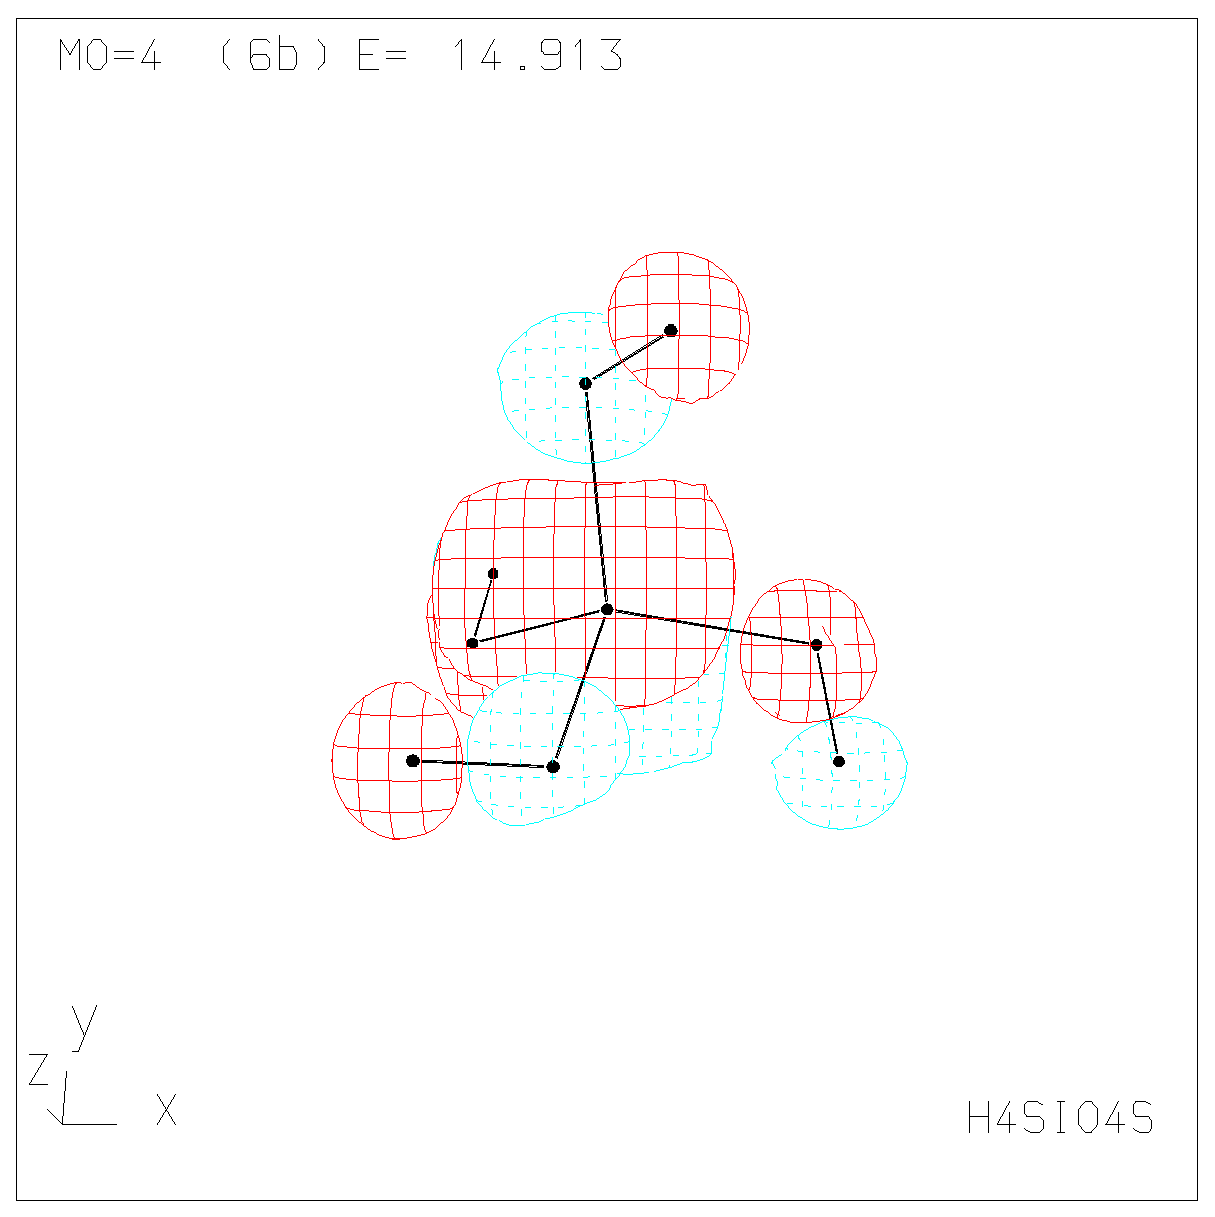
\includegraphics[width=5cm]{h4sio4_obrazky/s2_4.eps} \label{obr_h4sio4_MO_s2_4}}
\subfigure[MO 16]{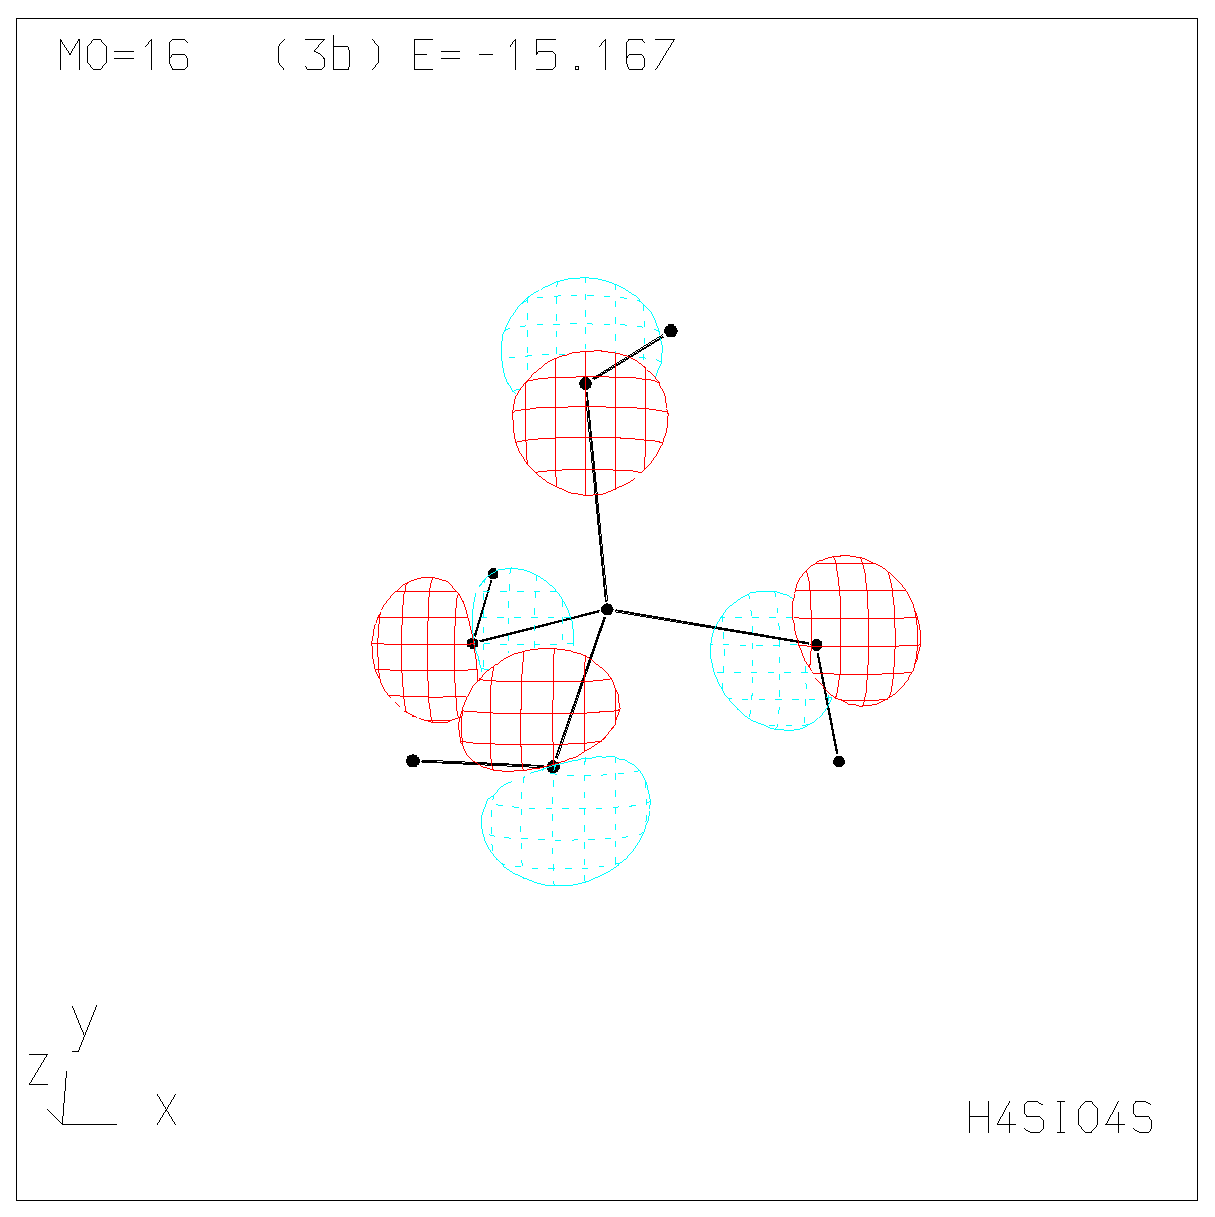
\includegraphics[width=5cm]{h4sio4_obrazky/s2_16.eps}\label{obr_h4sio4_MO_s2_16}}
\subfigure[MO 21]{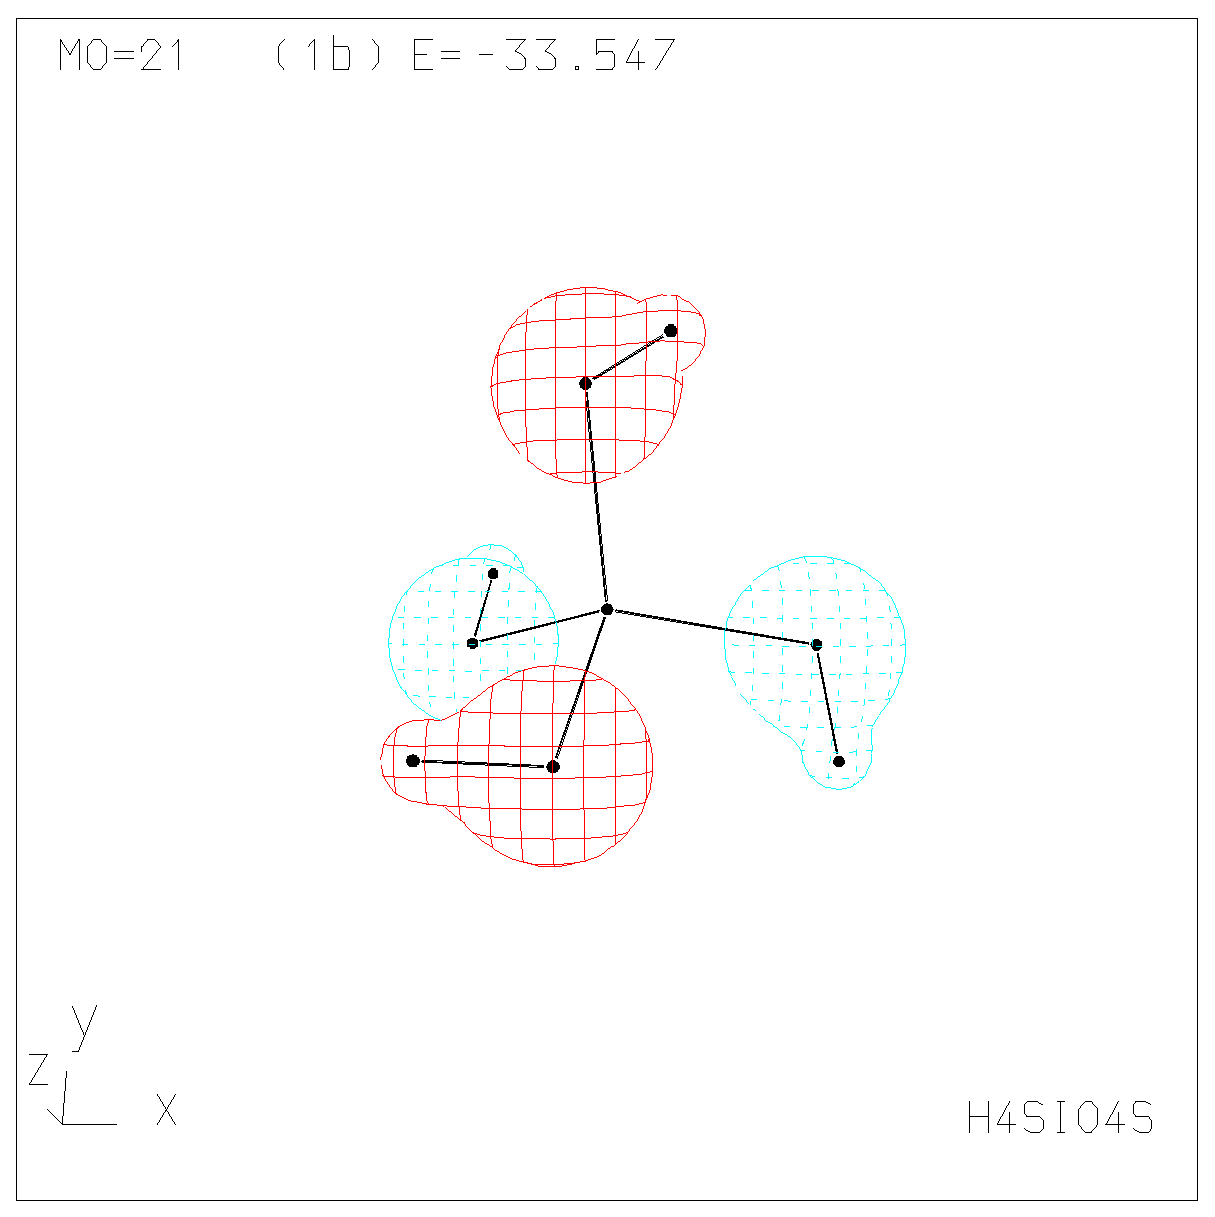
\includegraphics[width=5cm]{h4sio4_obrazky/s2_21.eps}\label{obr_h4sio4_MO_s2_21}}
\caption{Interakce $\bra{11}{\hat{H}}\ket{21}$, $\bra{19}{\hat{H}}\ket{21}$ z tabulky \ref{tab_h4sio4_vysledky}.}

\label{obr_h4sio4_vysledky_II}\end{center}
\end{figure}

%------------    
Fragmentové orbitaly  15, 18 a 22 se navzájem mísí za vzniku MO číslo 2, 19 a 22, znázorněných na obrázku \ref{obr_h4sio4_vysledky_III}.   
\begin{figure}
\begin{center}
\subfigure[MO 2]{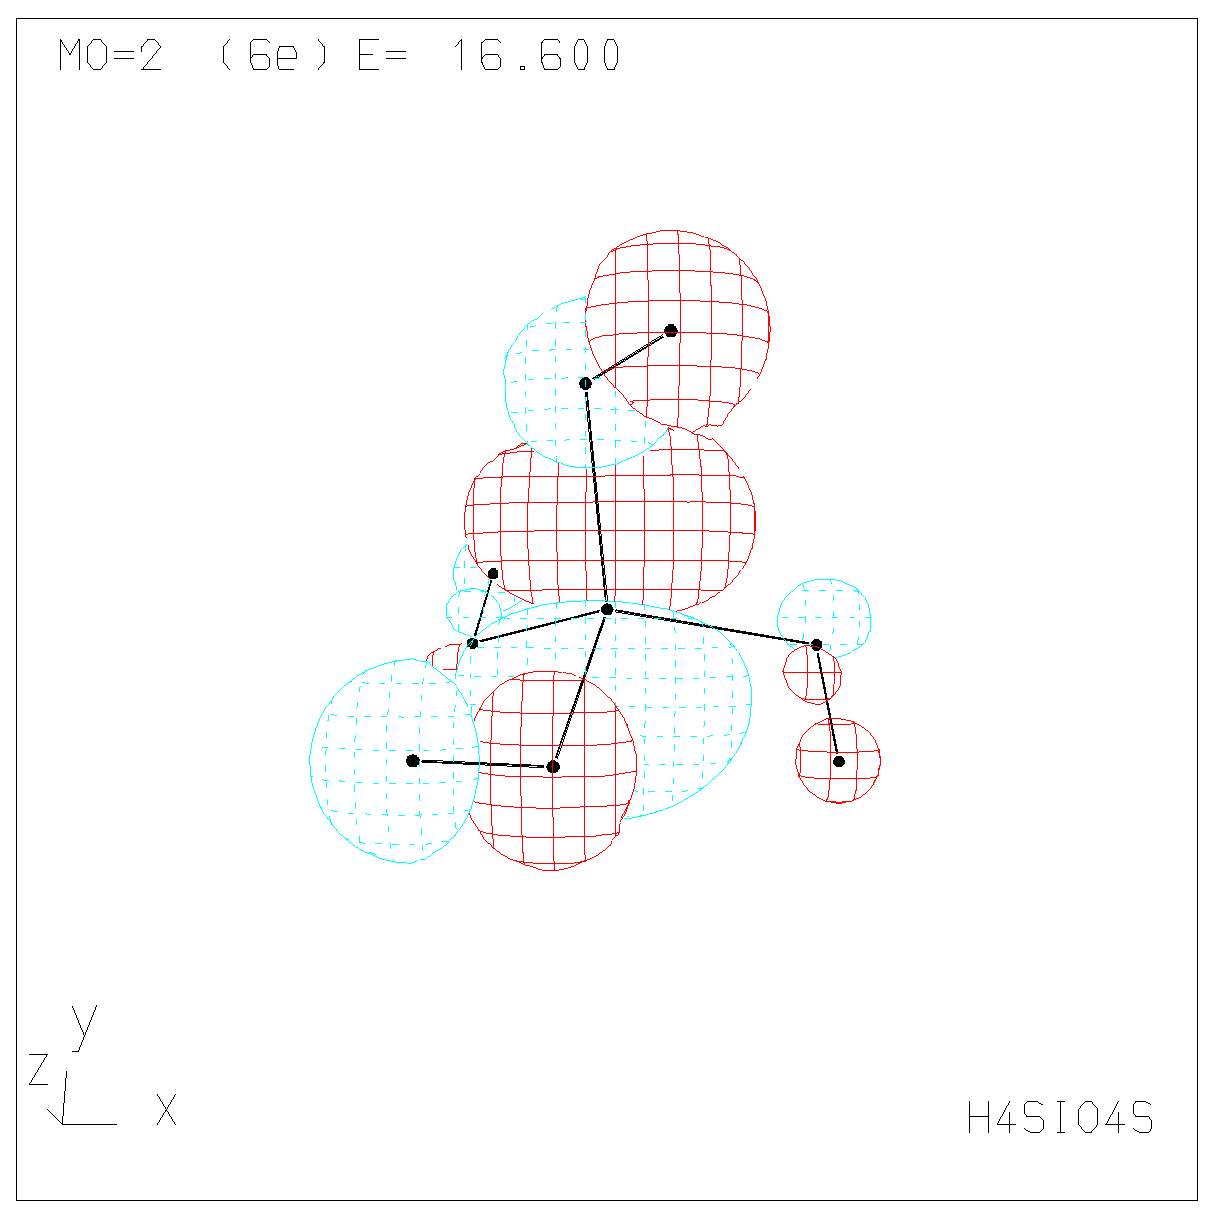
\includegraphics[width=5cm]{h4sio4_obrazky/s3__2.eps} \label{obr_h4sio4_MO_s3_2}}
\subfigure[MO 19]{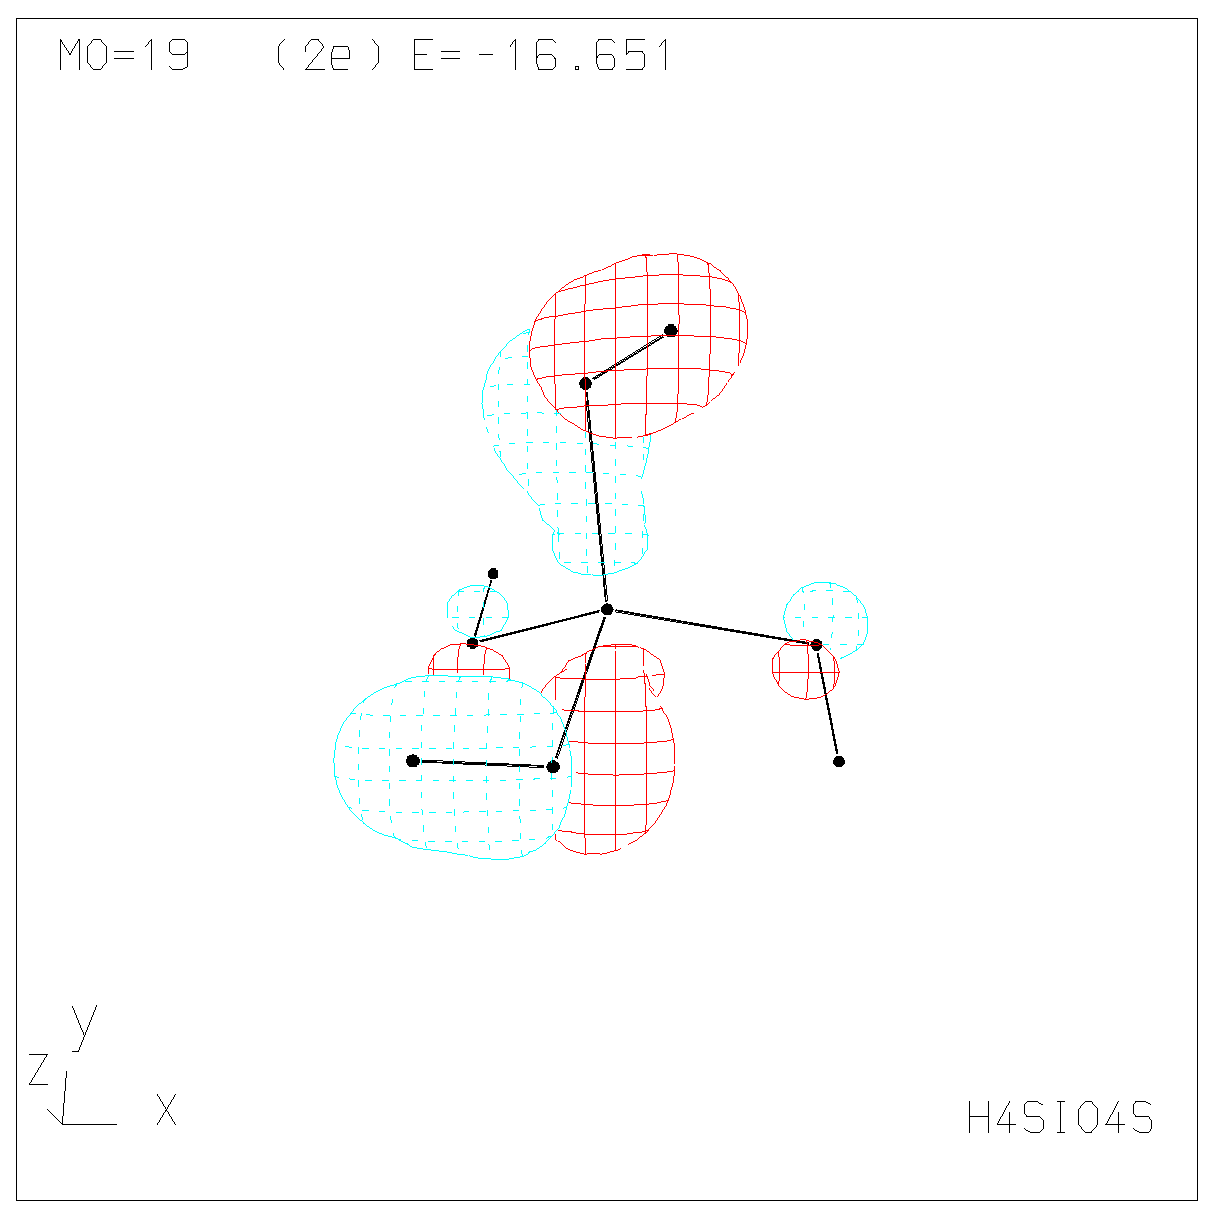
\includegraphics[width=5cm]{h4sio4_obrazky/s3__19.eps}\label{obr_h4sio4_MO_s3_19}}
\subfigure[MO 22]{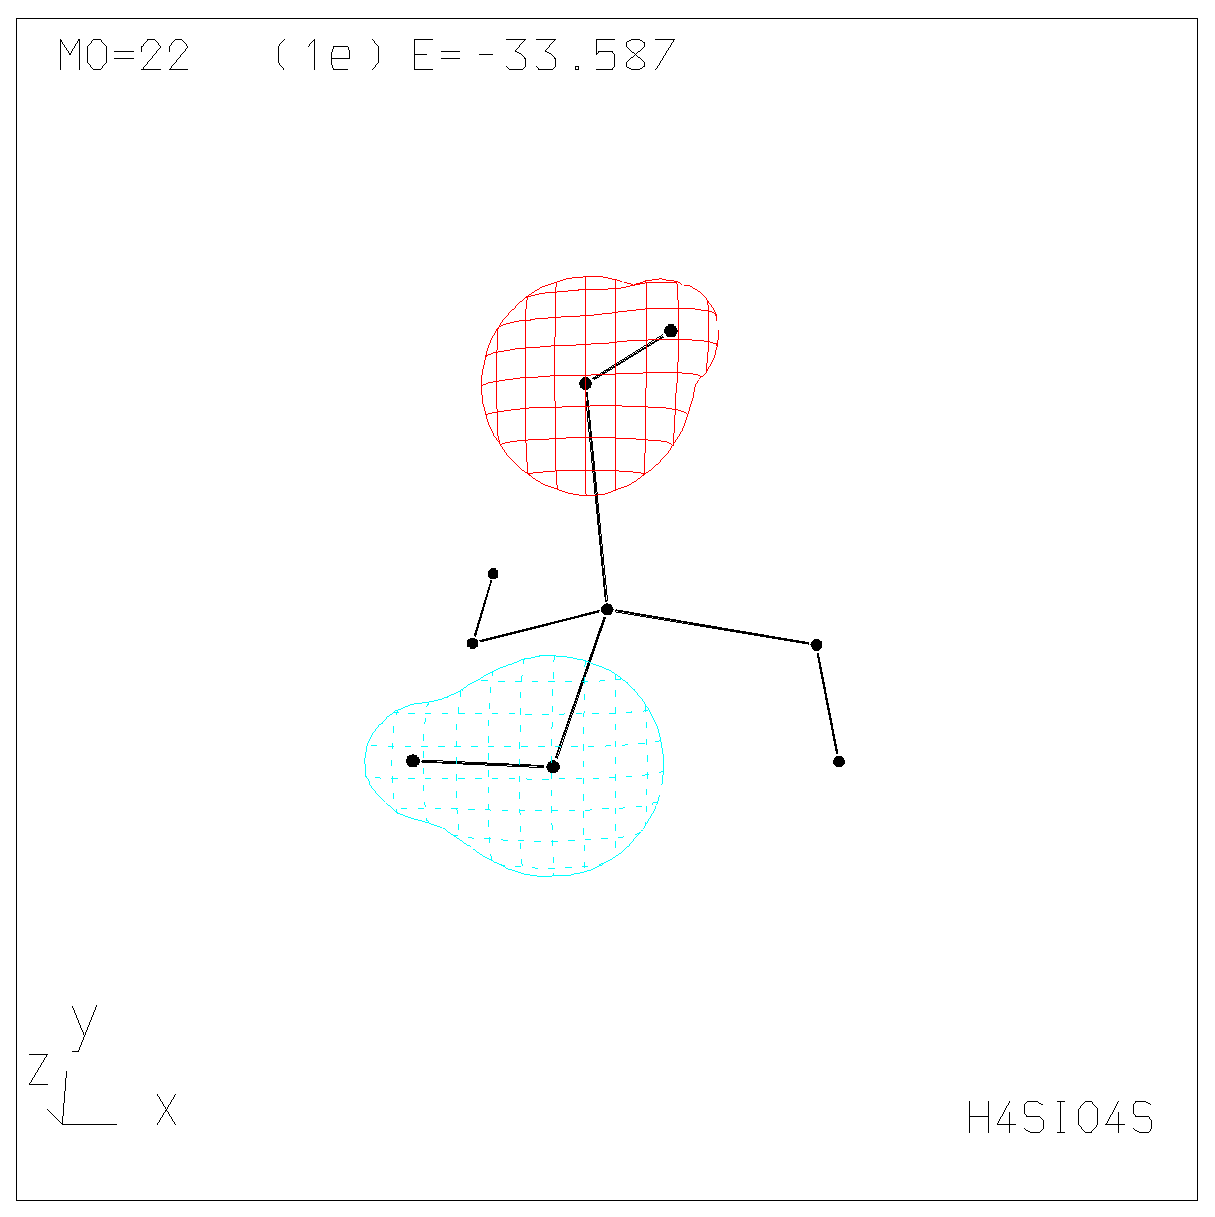
\includegraphics[width=5cm]{h4sio4_obrazky/s3__22.eps}\label{obr_h4sio4_MO_s2_21}}
\caption{Interakce $\bra{15}{\hat{H}}\ket{22}$, $\bra{18}{\hat{H}}\ket{22}$ z tabulky \ref{tab_h4sio4_vysledky}.}
\label{obr_h4sio4_vysledky_III}
\end{center}
\end{figure} 
%-------------------------------------------------------------------------------------
\subsection{Molekula Si(OH)$_3$CH$_3$}
\begin{figure}[h!]
\caption{Optimalizovaná struktura \ce{Si(OH)3CH3}. }
  \center
  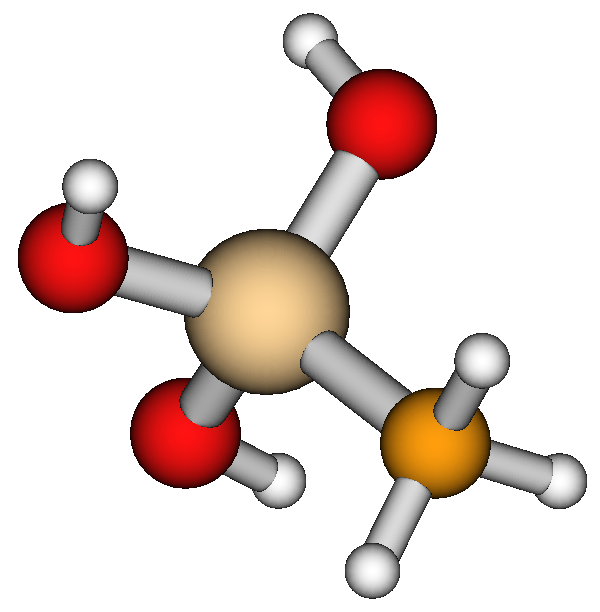
\includegraphics[width=5cm]{si(oh)3ch3_obr.png}
  \label{obr_sioh3ch3_opt_struktura}
  \end{figure}
  
\begin{table}[htbp]
\caption{Výsledné mísení orbitalů pro \ce{Si(OH)3CH3}}
\begin{center}
\begin{tabular}{|r|r|r|r|r|r|r|r|}
\hline
\multicolumn{2}{|c|}{$\bra{22}{\hat{H}}\ket{26}$, $\bra{7}{\hat{H}}\ket{26}$} & \multicolumn{2}{|c|}{$\bra{7}{\hat{H}}\ket{25}$}& \multicolumn{2}{|c|}{$\bra{21}{\hat{H}}\ket{23}$} &\multicolumn{2}{|c|}{$\bra{20}{\hat{H}}\ket{24}$} \\
\hline
\hline
\multicolumn{1}{|l|}{MO} & \multicolumn{1}{r|}{W} & \multicolumn{1}{l|}{MO} & \multicolumn{1}{r|}{W} & MO & \multicolumn{1}{r|}{W}& MO & \multicolumn{1}{r|}{W} \\ \hline
3 & 46 \% & 11 & 79 \% &25 & 100 \%& 24 & 100 \% \\ \hline
11 & 71 \% & 5 & 40 \% & 2 & 34 \% &4 & 58 \% \\ \hline
26 & 98 \% & - & - &  -& - &-&- \\ \hline
\end{tabular}
\end{center}
\label{tab_sioh3ch3_vysledky}
\end{table}

Fragmentové orbitaly  7, 22 a 26 se navzájem mísí za vzniku MO číslo 3, 11 a 26, znázorněných na obrázku \ref{obr_sioh3ch3_vysledky_I}.   
\begin{figure}
\begin{center}
\subfigure[MO 3]{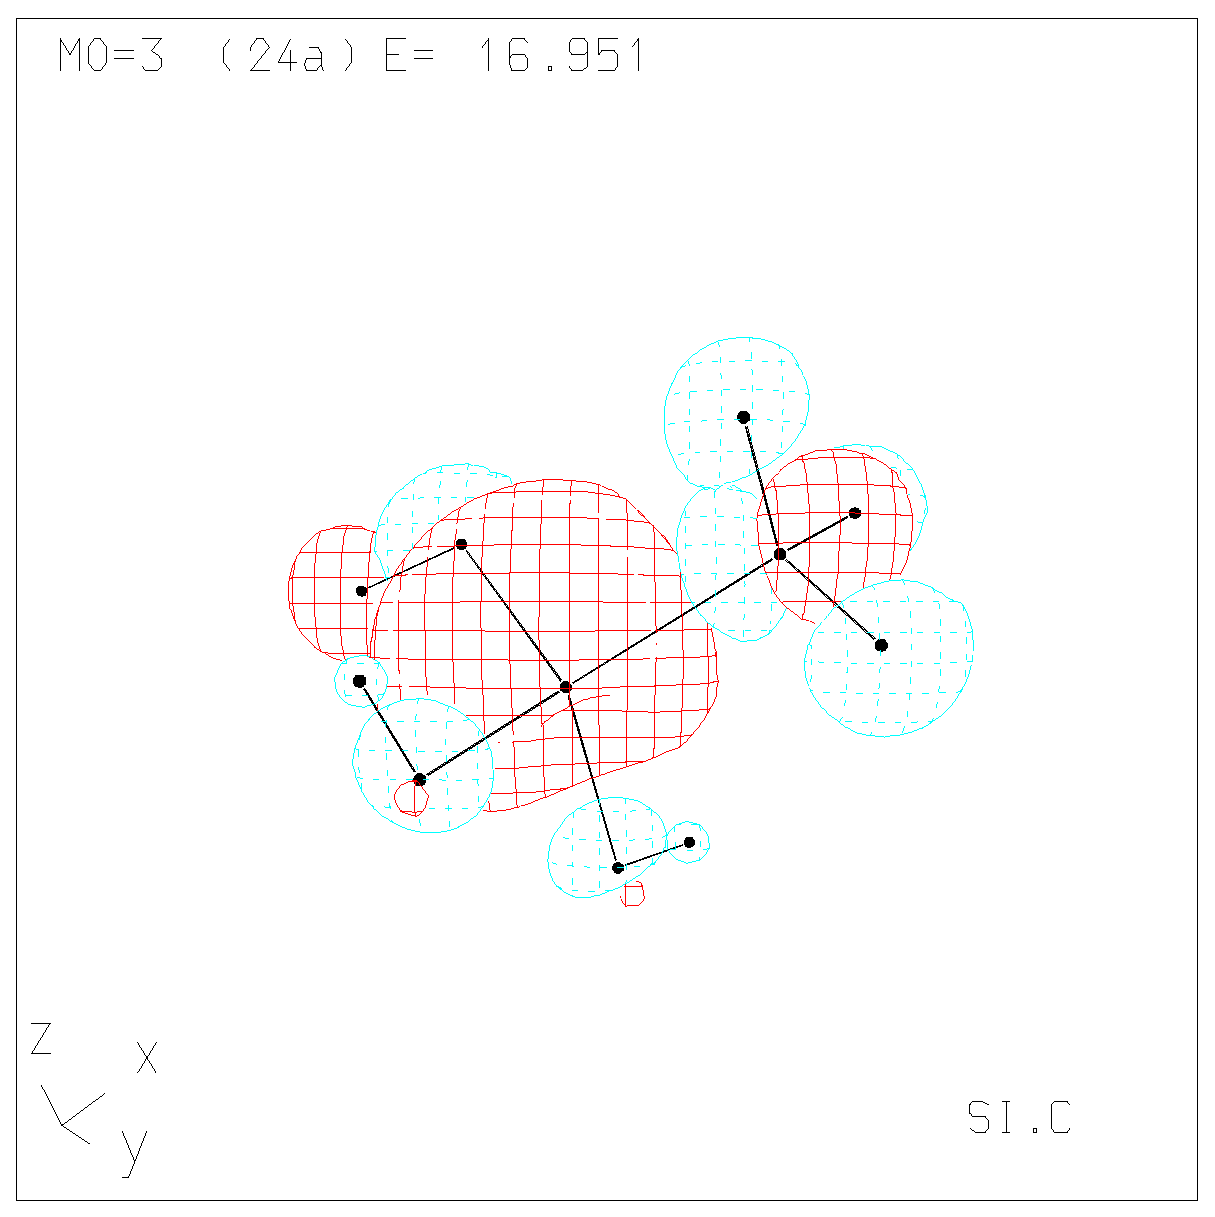
\includegraphics[width=5cm]{sioh3ch3_obrazky/s1_3.eps} \label{obr_sioh3ch3_MO_s1_3}}
\subfigure[MO 11]{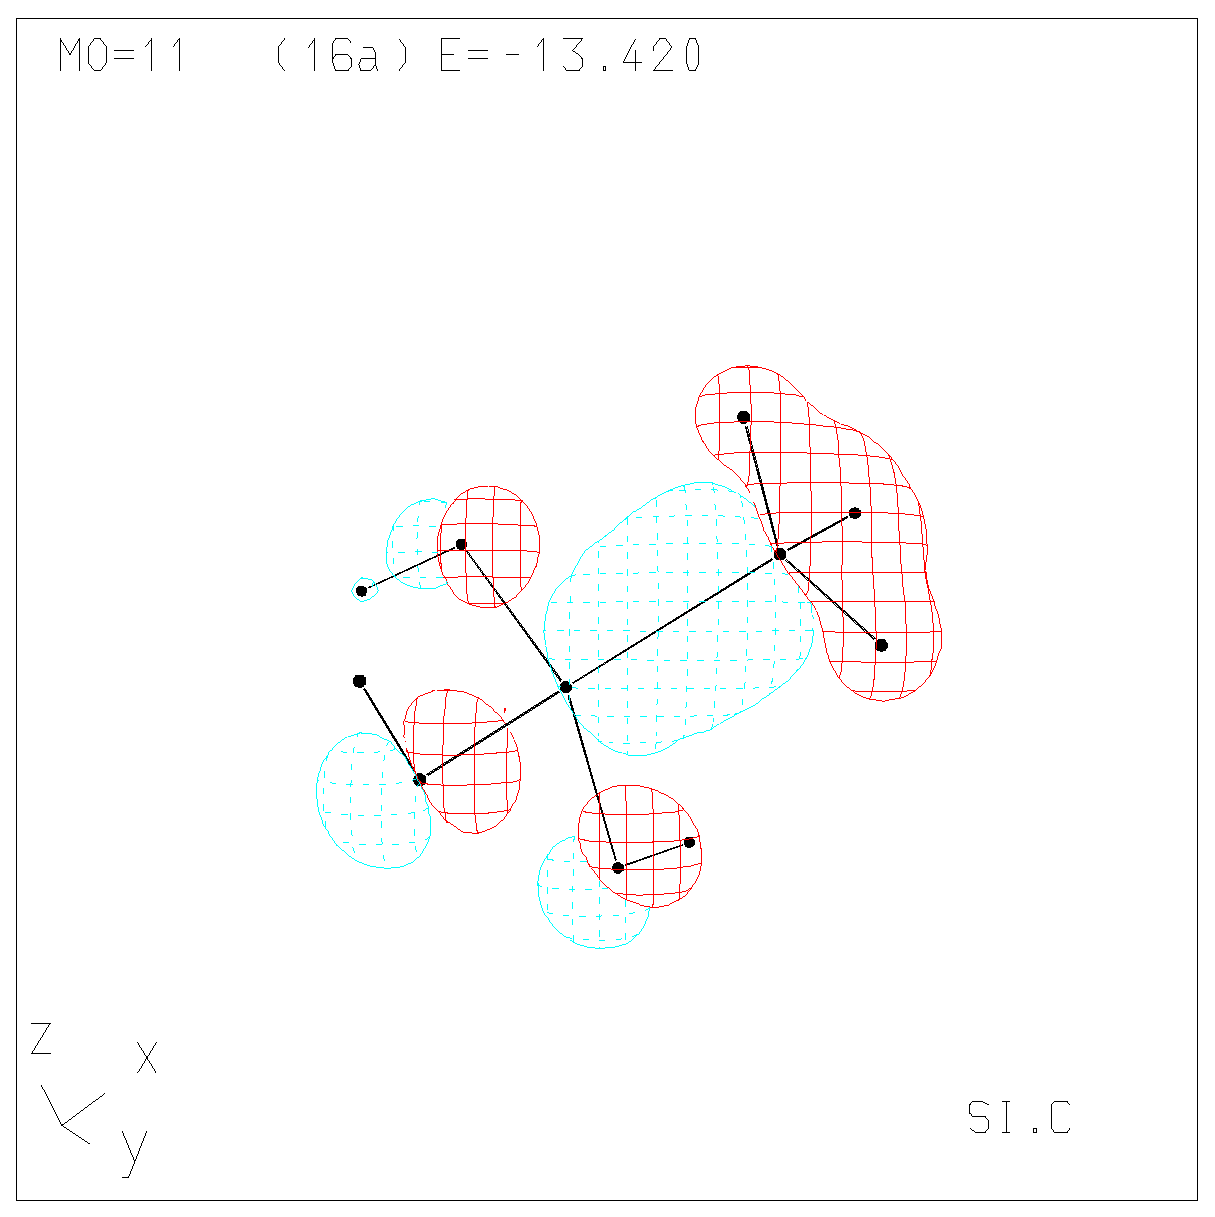
\includegraphics[width=5cm]{sioh3ch3_obrazky/s1_11.eps}\label{obr_sioh3ch3_MO_s1_11}}
\subfigure[MO 26]{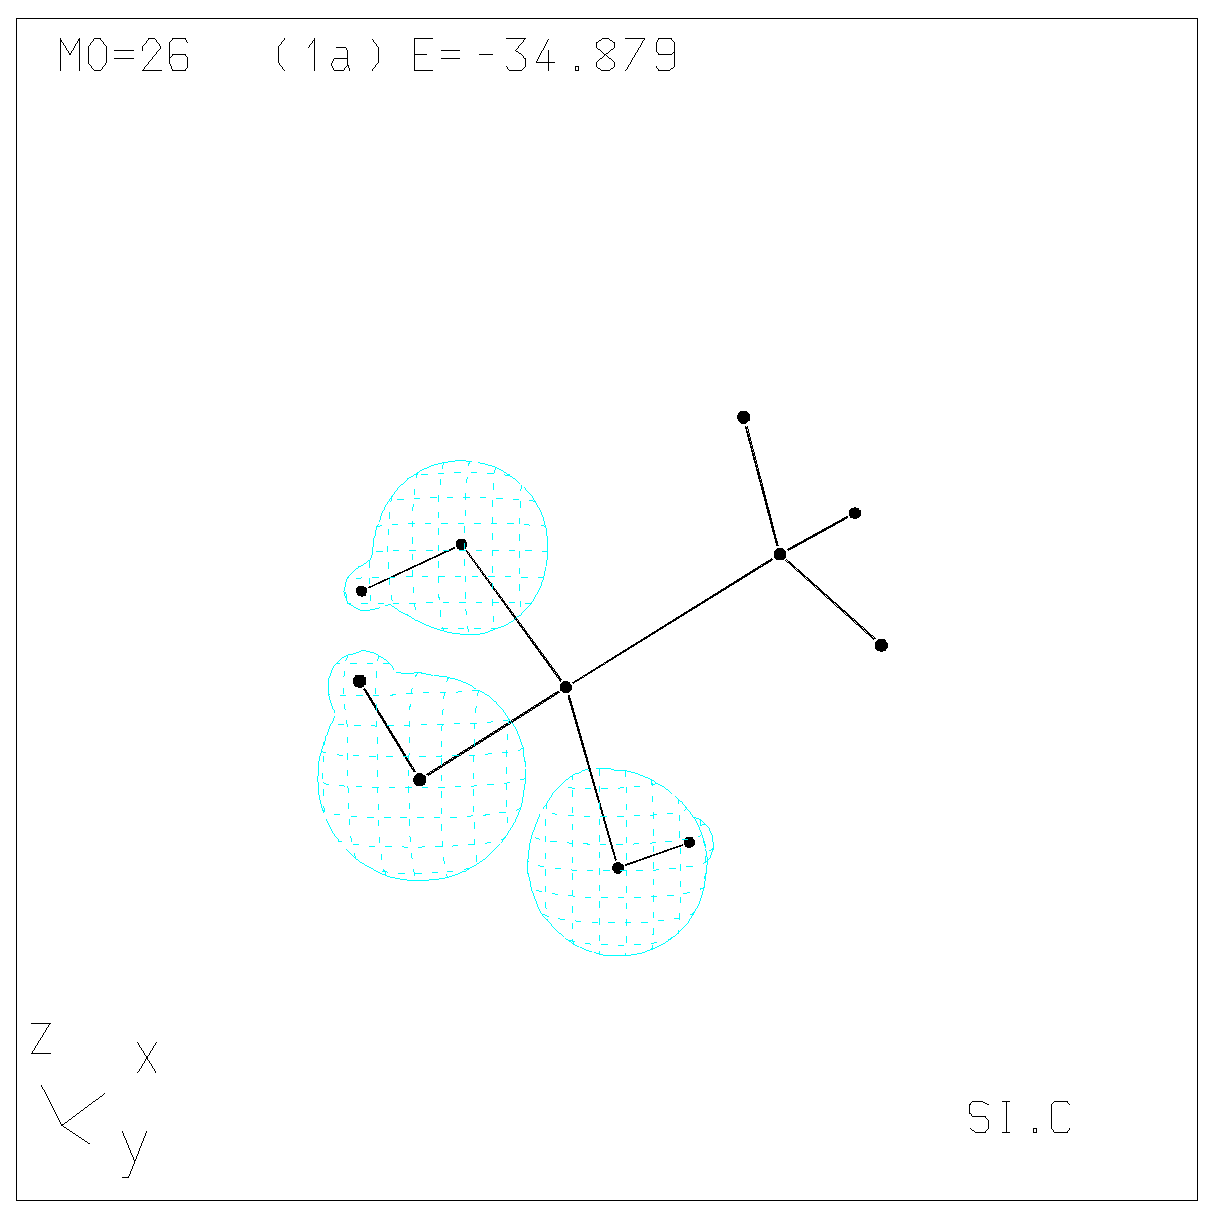
\includegraphics[width=5cm]{sioh3ch3_obrazky/s1_26.eps}\label{obr_sioh3ch3_MO_s1_26}}
\caption{Interakce $\bra{22}{\hat{H}}\ket{26}$, $\bra{7}{\hat{H}}\ket{26}$  z tabulky \ref{tab_sioh3ch3_vysledky}.}

\label{obr_sioh3ch3_vysledky_I}\end{center}
\end{figure} 

Fragmentové orbitaly  7 a 25 se navzájem mísí za vzniku MO číslo 5 a 11, znázorněných na obrázku \ref{obr_sioh3ch3_vysledky_II}.   
\begin{figure}
\begin{center}
\subfigure[MO 5]{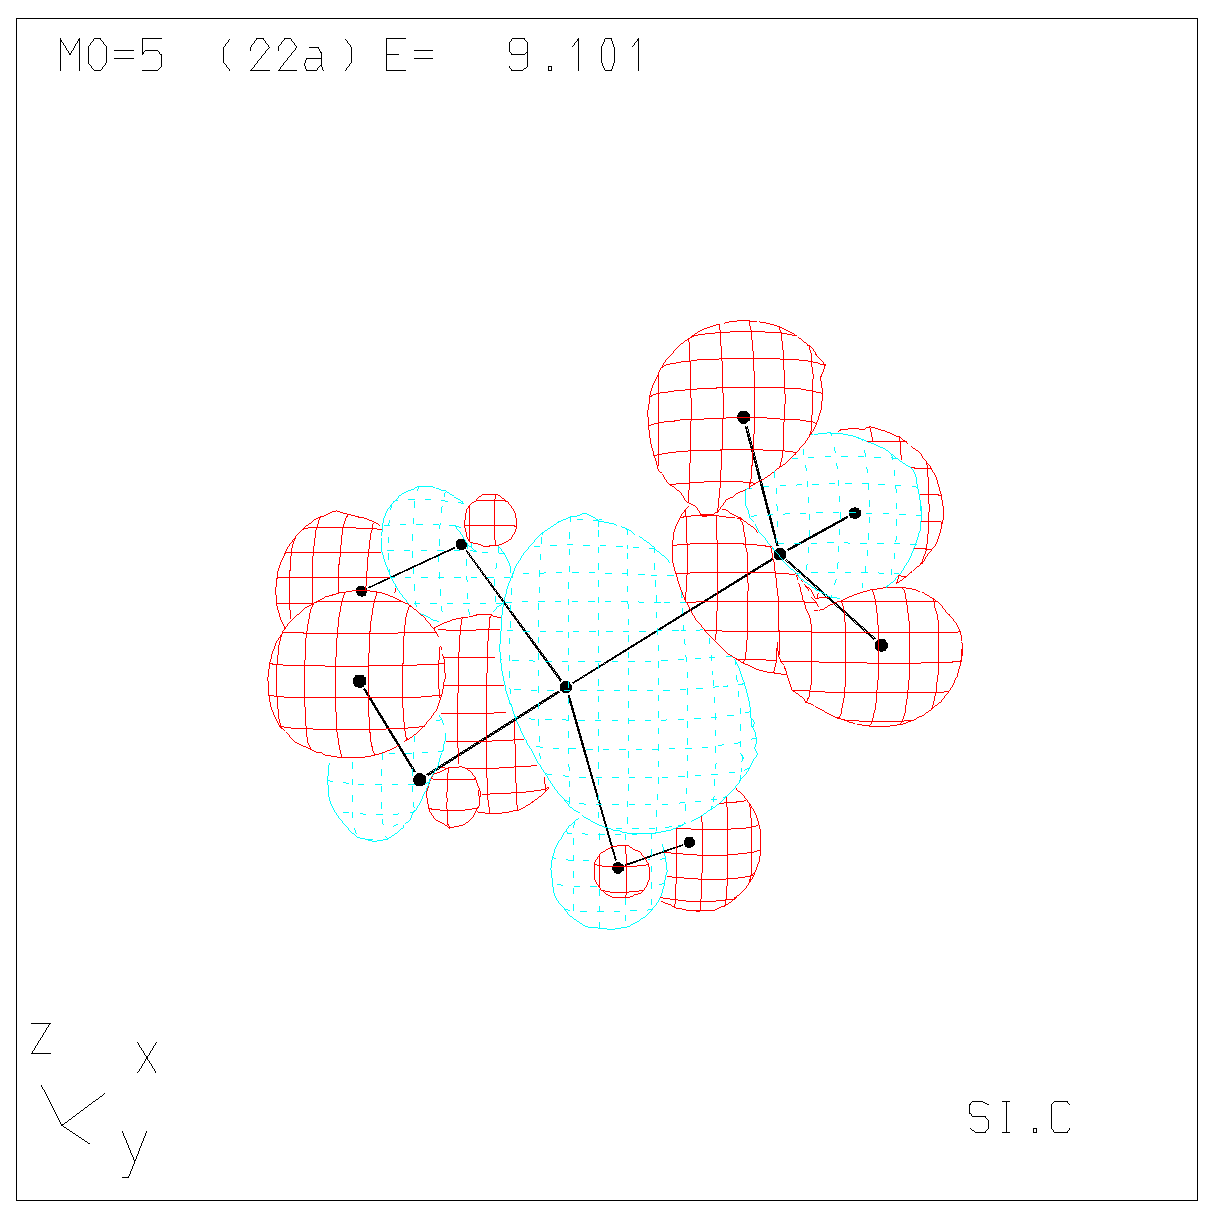
\includegraphics[width=5cm]{sioh3ch3_obrazky/s2_5.eps} \label{obr_sioh3ch3_MO_s2_5}}
\subfigure[MO 11]{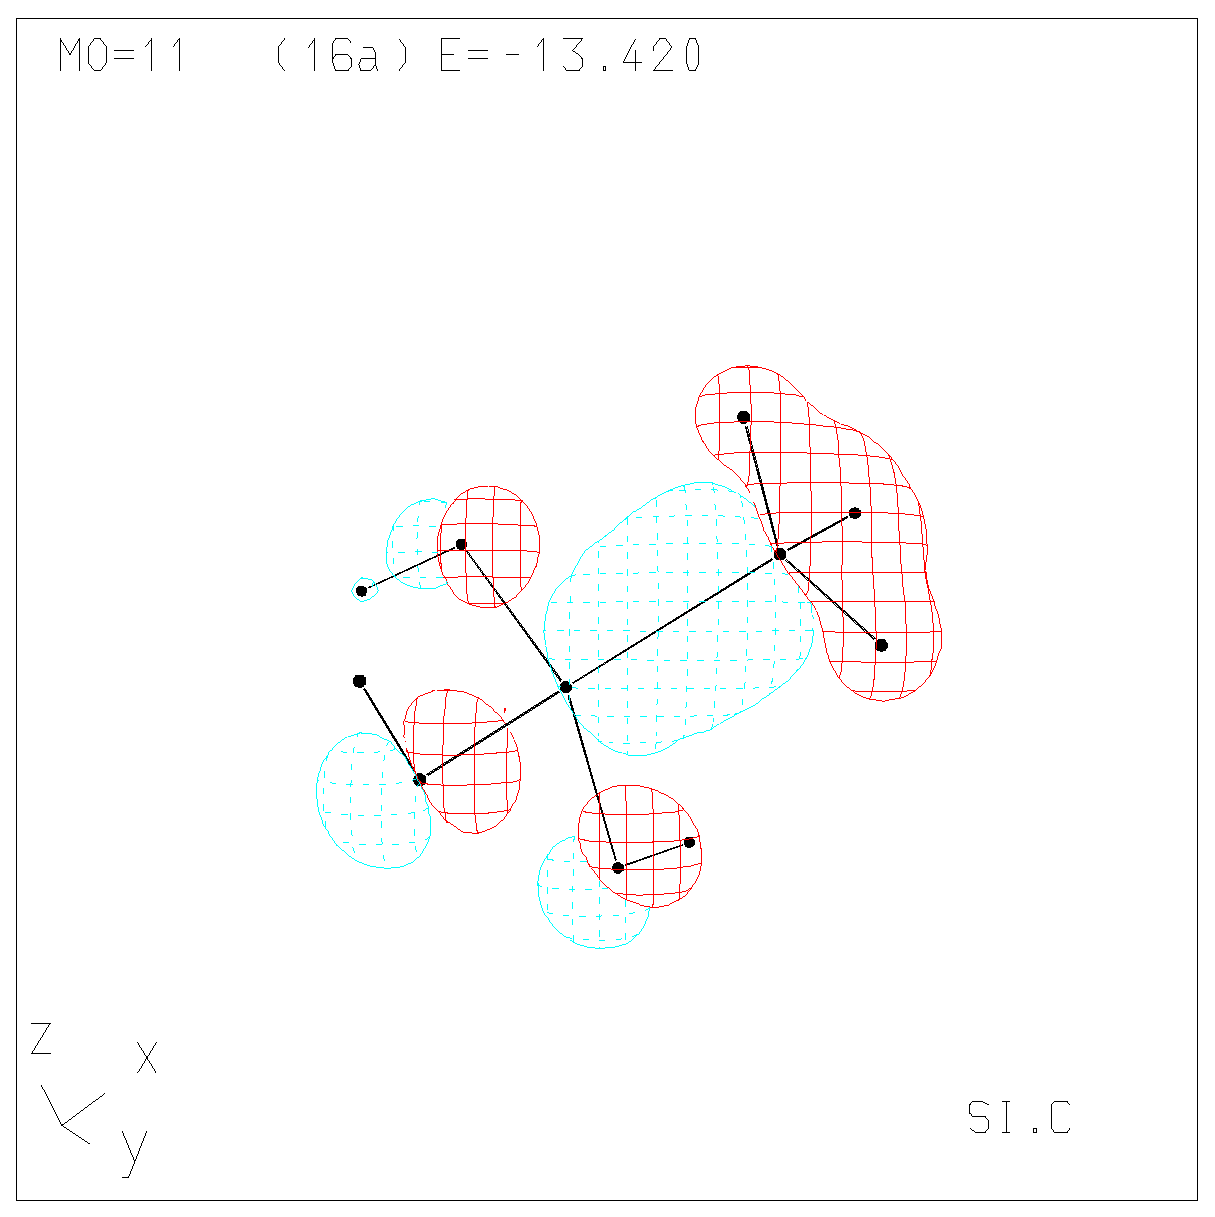
\includegraphics[width=5cm]{sioh3ch3_obrazky/s2_11.eps}\label{obr_sioh3ch3_MO_s2_11}}
\caption{Interakce $\bra{7}{\hat{H}}\ket{25}$ z tabulky \ref{tab_sioh3ch3_vysledky}.}

\label{obr_sioh3ch3_vysledky_II}\end{center}
\end{figure} 

 \clearpage
   
Fragmentové orbitaly  21 a 23 se navzájem mísí za vzniku MO číslo 2 a 25, znázorněných na obrázku \ref{obr_sioh3ch3_vysledky_III}.   
\begin{figure}
\begin{center}
\subfigure[MO 5]{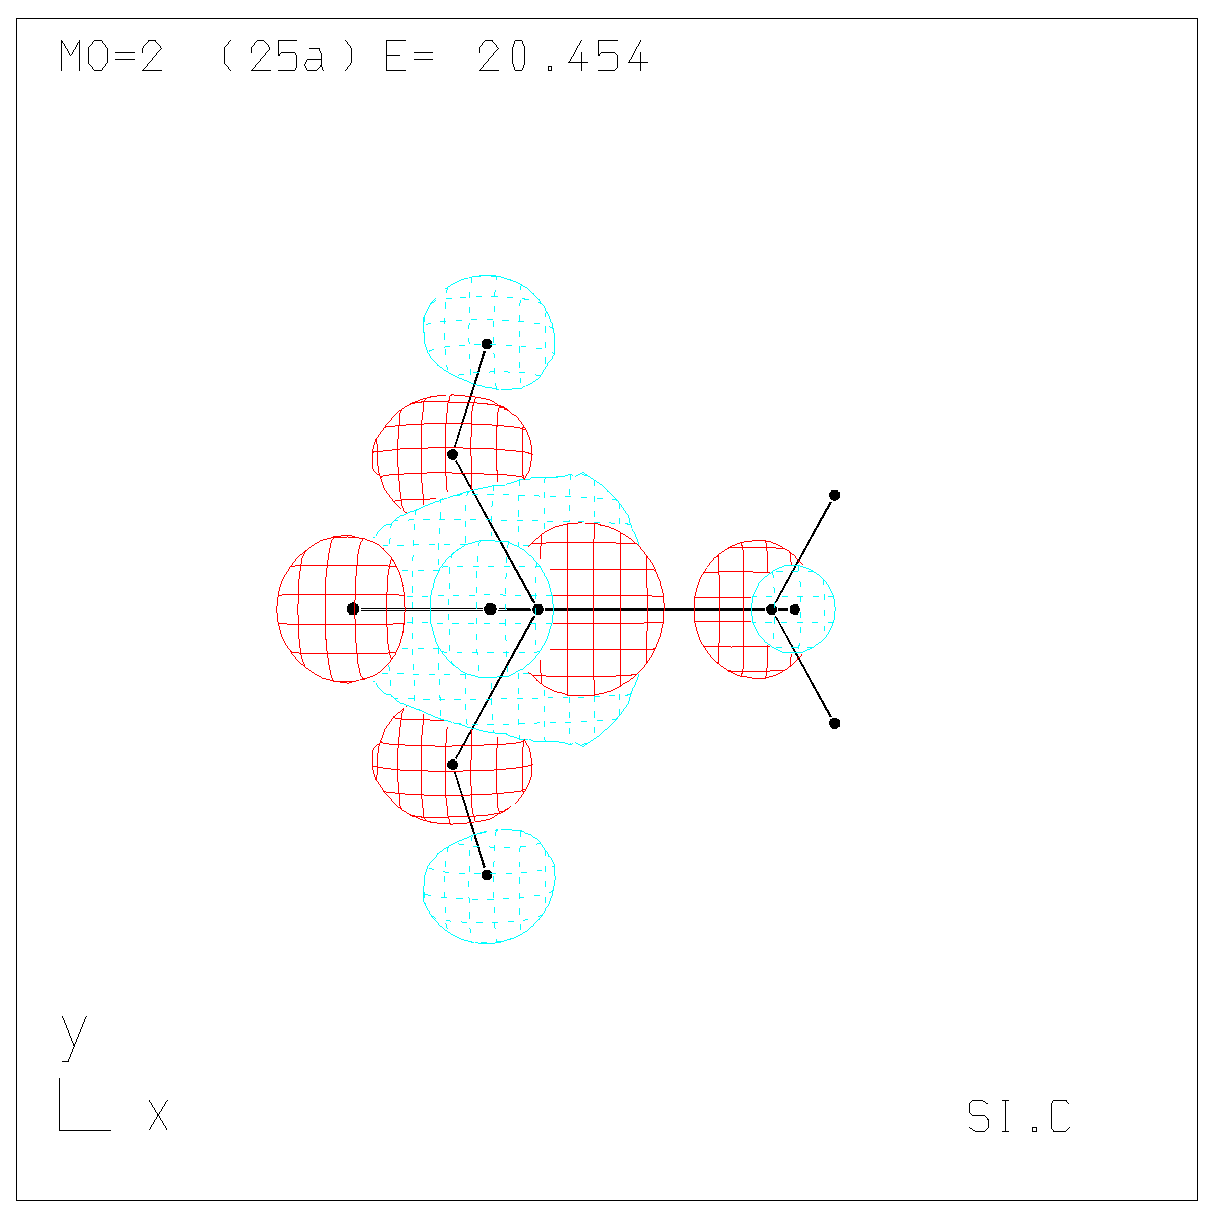
\includegraphics[width=5cm]{sioh3ch3_obrazky/s3_2.eps} \label{obr_sioh3ch3_MO_s3_2}}
\subfigure[MO 11]{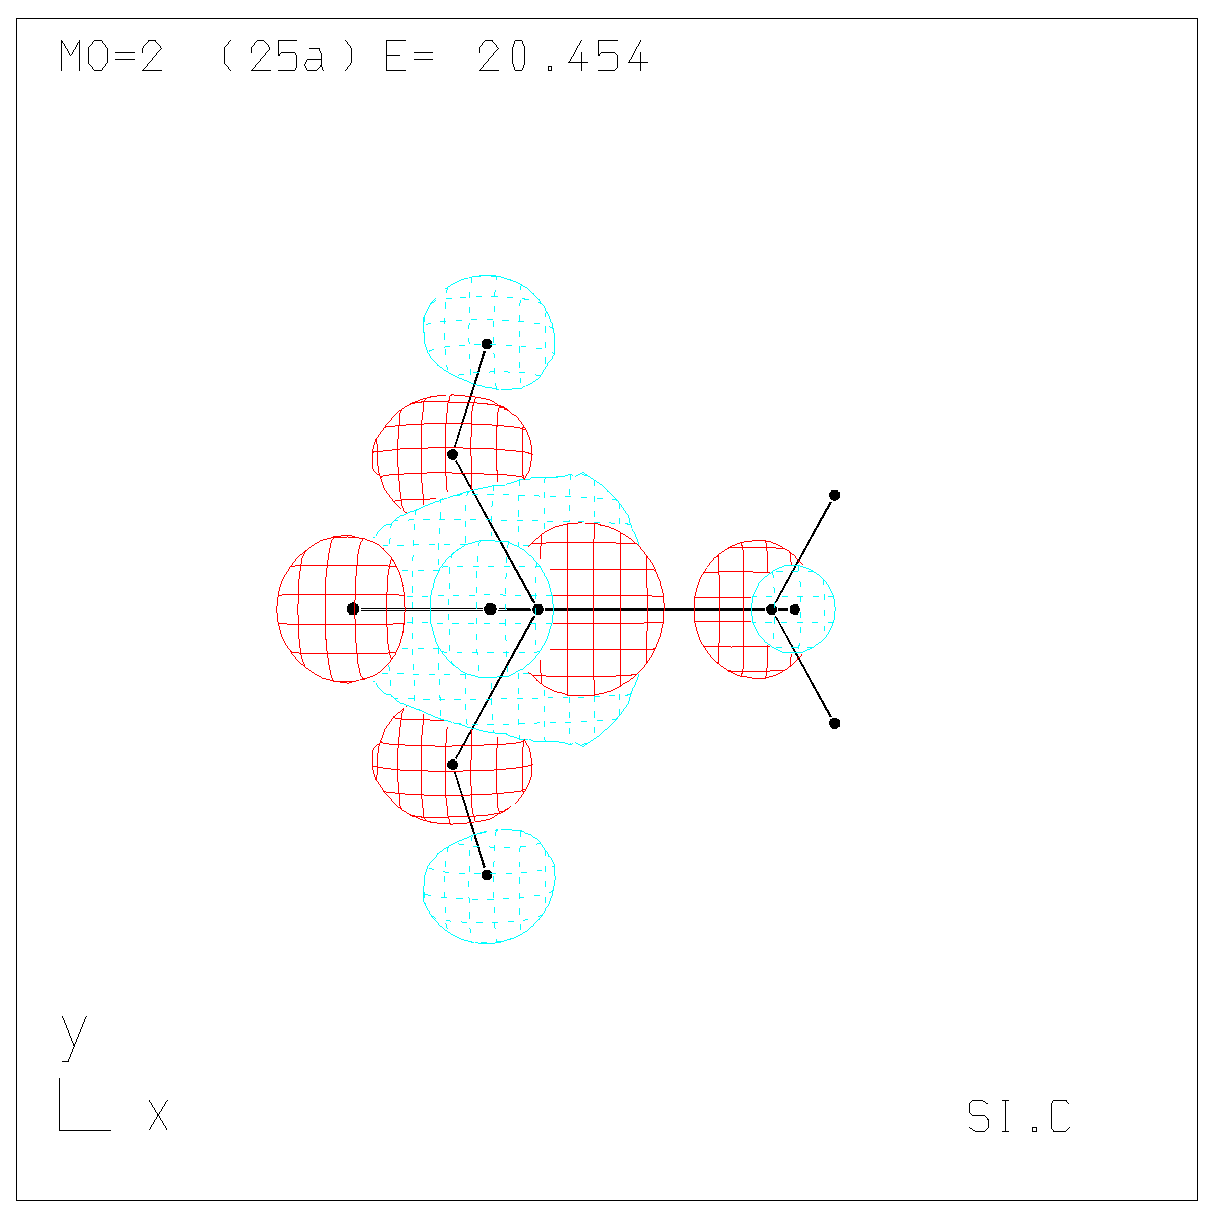
\includegraphics[width=5cm]{sioh3ch3_obrazky/s3_2.eps}\label{obr_sioh3ch3_MO_s3_25}}
\caption{Interakce $\bra{21}{\hat{H}}\ket{23}$  z tabulky \ref{tab_sioh3ch3_vysledky}.}

\label{obr_sioh3ch3_vysledky_III}\end{center}
\end{figure} 
   
Fragmentové orbitaly  20 a 24 se navzájem mísí za vzniku MO číslo 4 a 24, znázorněných na obrázku \ref{obr_sioh3ch3_vysledky_IV}.   
\begin{figure}
\begin{center}
\subfigure[MO 5]{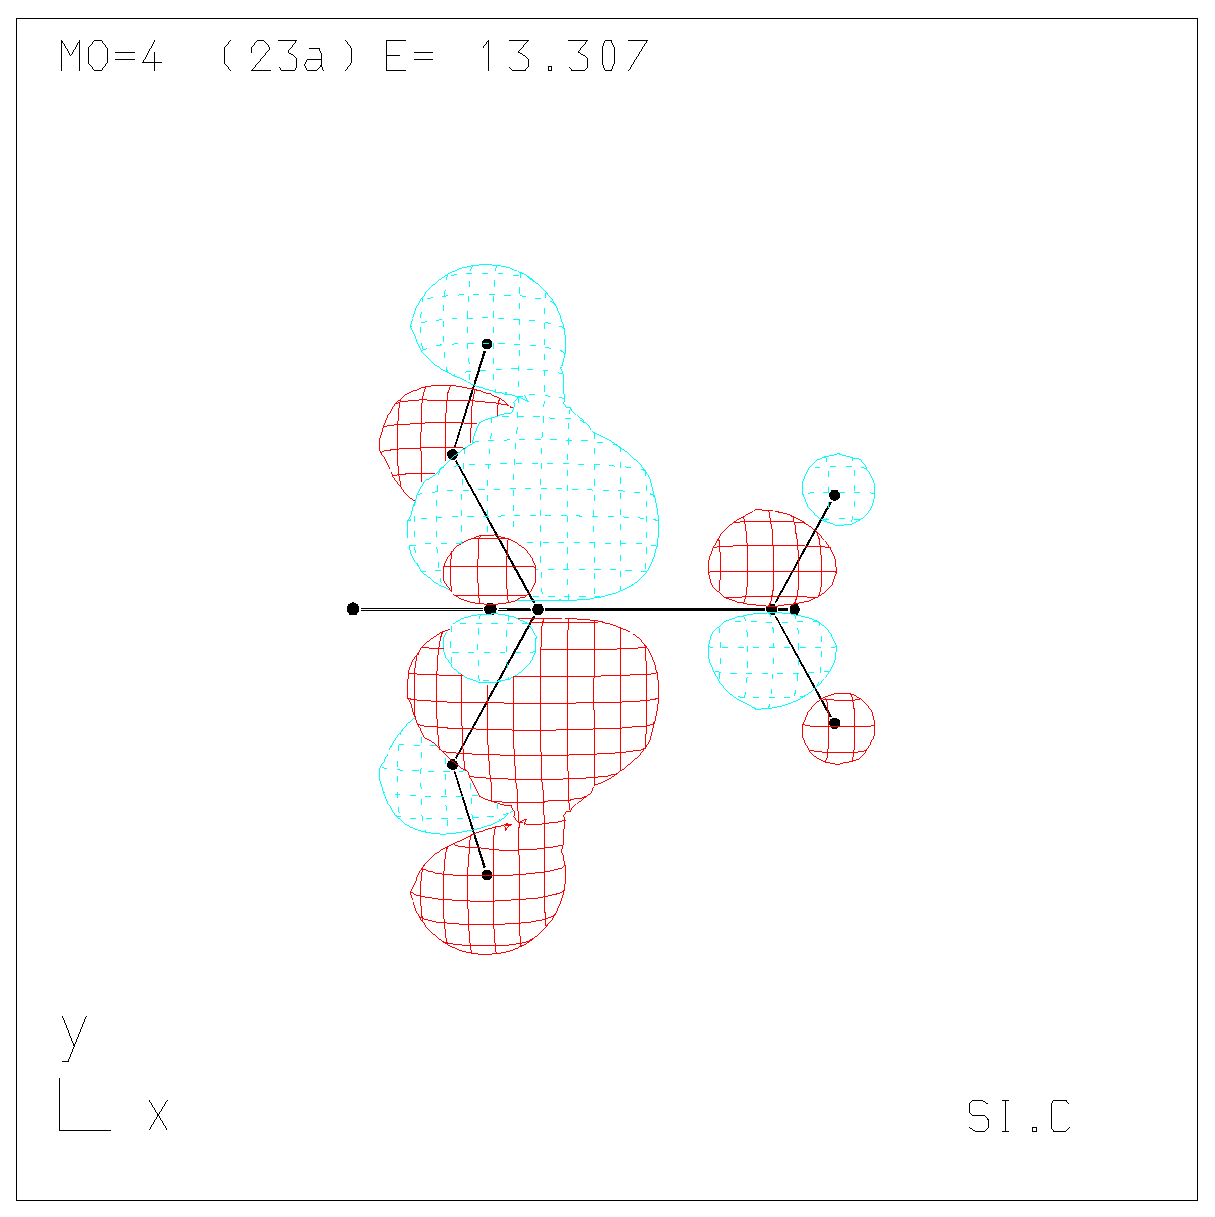
\includegraphics[width=5cm]{sioh3ch3_obrazky/s4_4.eps} \label{obr_sioh3ch3_MO_s4_4}}
\subfigure[MO 11]{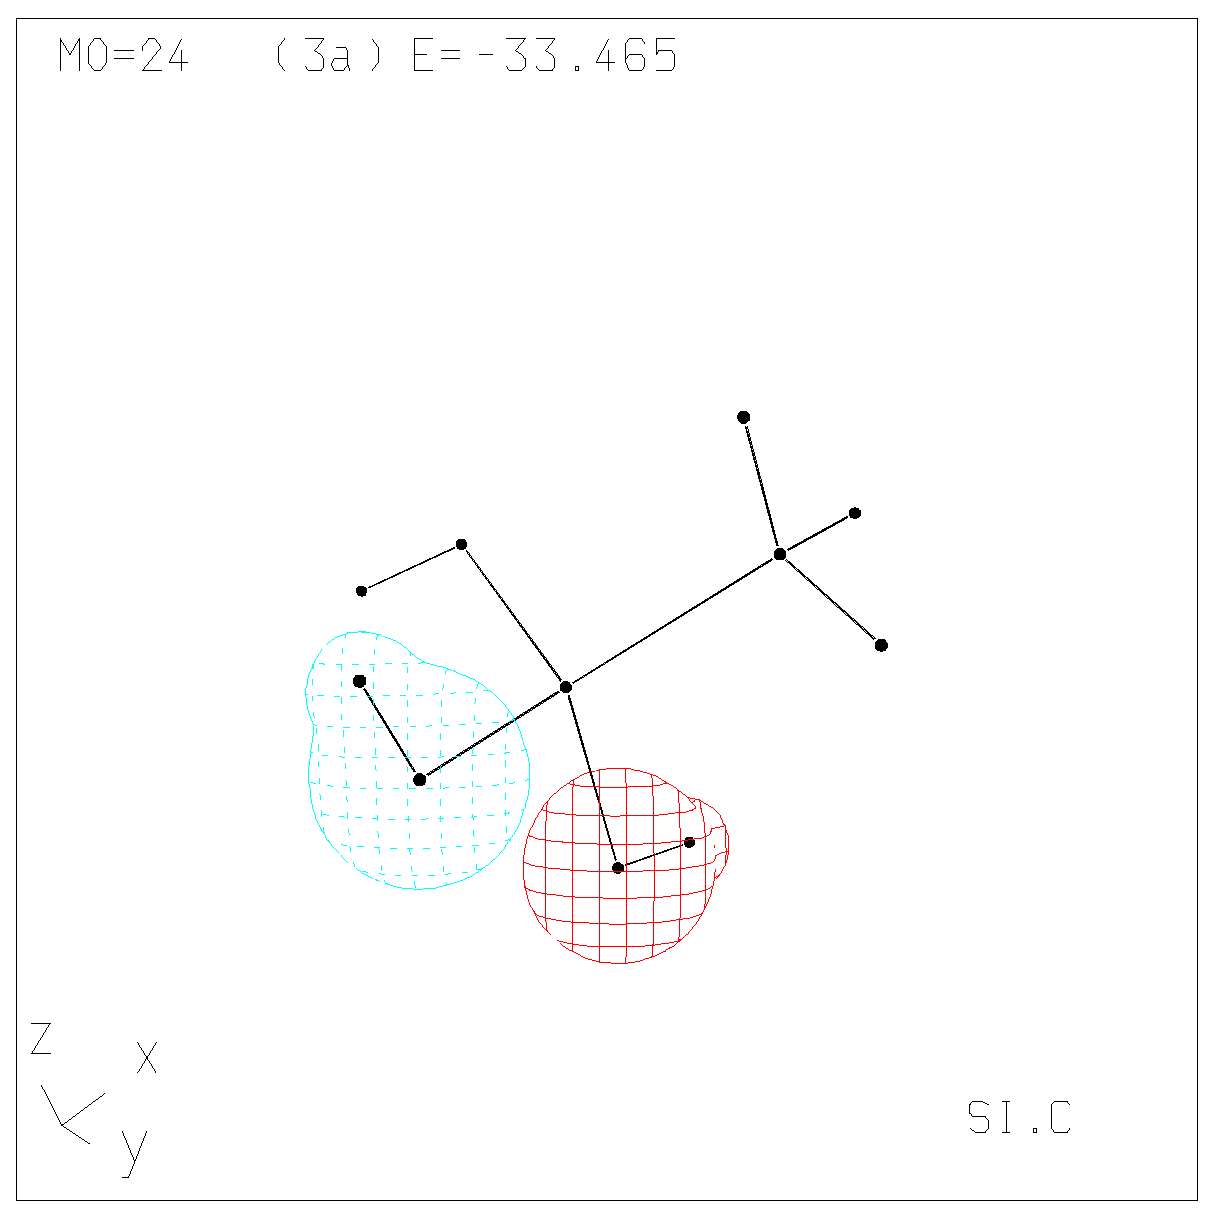
\includegraphics[width=5cm]{sioh3ch3_obrazky/s4_24.eps}\label{obr_sioh3ch3_MO_s4_24}}
\caption{Interakce $\bra{20}{\hat{H}}\ket{24}$  z tabulky \ref{tab_sioh3ch3_vysledky}.}

\label{obr_sioh3ch3_vysledky_IV}\end{center}
\end{figure} 
 %-------------------------------------------------------------------------------------------- 
  \subsection{Molekula H$_6$SiO$_6$}
   \subsection{Molekula H$_6$SiO$_6$}
 \begin{figure}[h!]
\caption{Optimalizovaná struktura \ce{H6SiO6}. }
  \center
  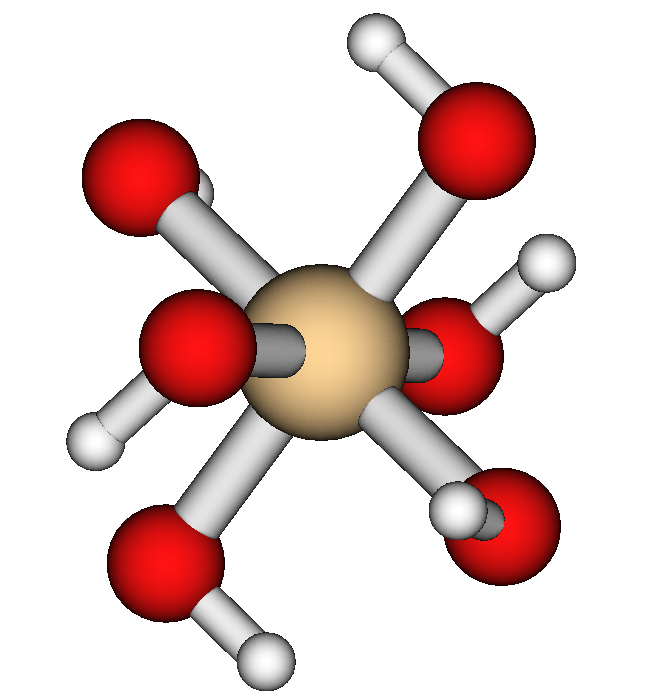
\includegraphics[width=5cm]{obr_h6sio6.png}
  \label{obr_h6sio6_opt_struktura}
  \end{figure}
 
  
  \begin{table}[htbp]
\caption{Výsledné mísení orbitalů pro \ce{(H6SiO6)^-2}}
\begin{center}
\begin{tabular}{|r|r|r|r|r|r|}
\hline
\multicolumn{2}{|c}{$\bra{30}{\hat{H}}\ket{34}$, $\bra{24}{\hat{H}}\ket{34}$} & \multicolumn{2}{|c|}{$\bra{21}{\hat{H}}\ket{32}$, $\bra{28}{\hat{H}}\ket{32}$}& \multicolumn{2}{|c|}{$\bra{22}{\hat{H}}\ket{33}$} \\
\hline \hline
\multicolumn{1}{|l|}{MO} & \multicolumn{1}{r|}{W} & \multicolumn{1}{l|}{MO} & \multicolumn{1}{r|}{W} & MO & \multicolumn{1}{r|}{W} \\ \hline
1 & 96 \% & 3 & 86 \% &2 & 65 \% \\ \hline
28 & 84 \% & 26 & 97 \% & - & - \\ \hline
34 & 100 \% & 32 & 99 \% &  -& - \\ \hline
\end{tabular}

\label{tab_h6sio6_vysledky}\end{center}
\end{table}
   
Fragmentové orbitaly  24, 30 a 34 se navzájem mísí za vzniku MO číslo 1, 28 a 34 znázorněných na obrázku \ref{obr_h6sio6_vysledky_I}.   
\begin{figure}
\begin{center}
\subfigure[MO 5]{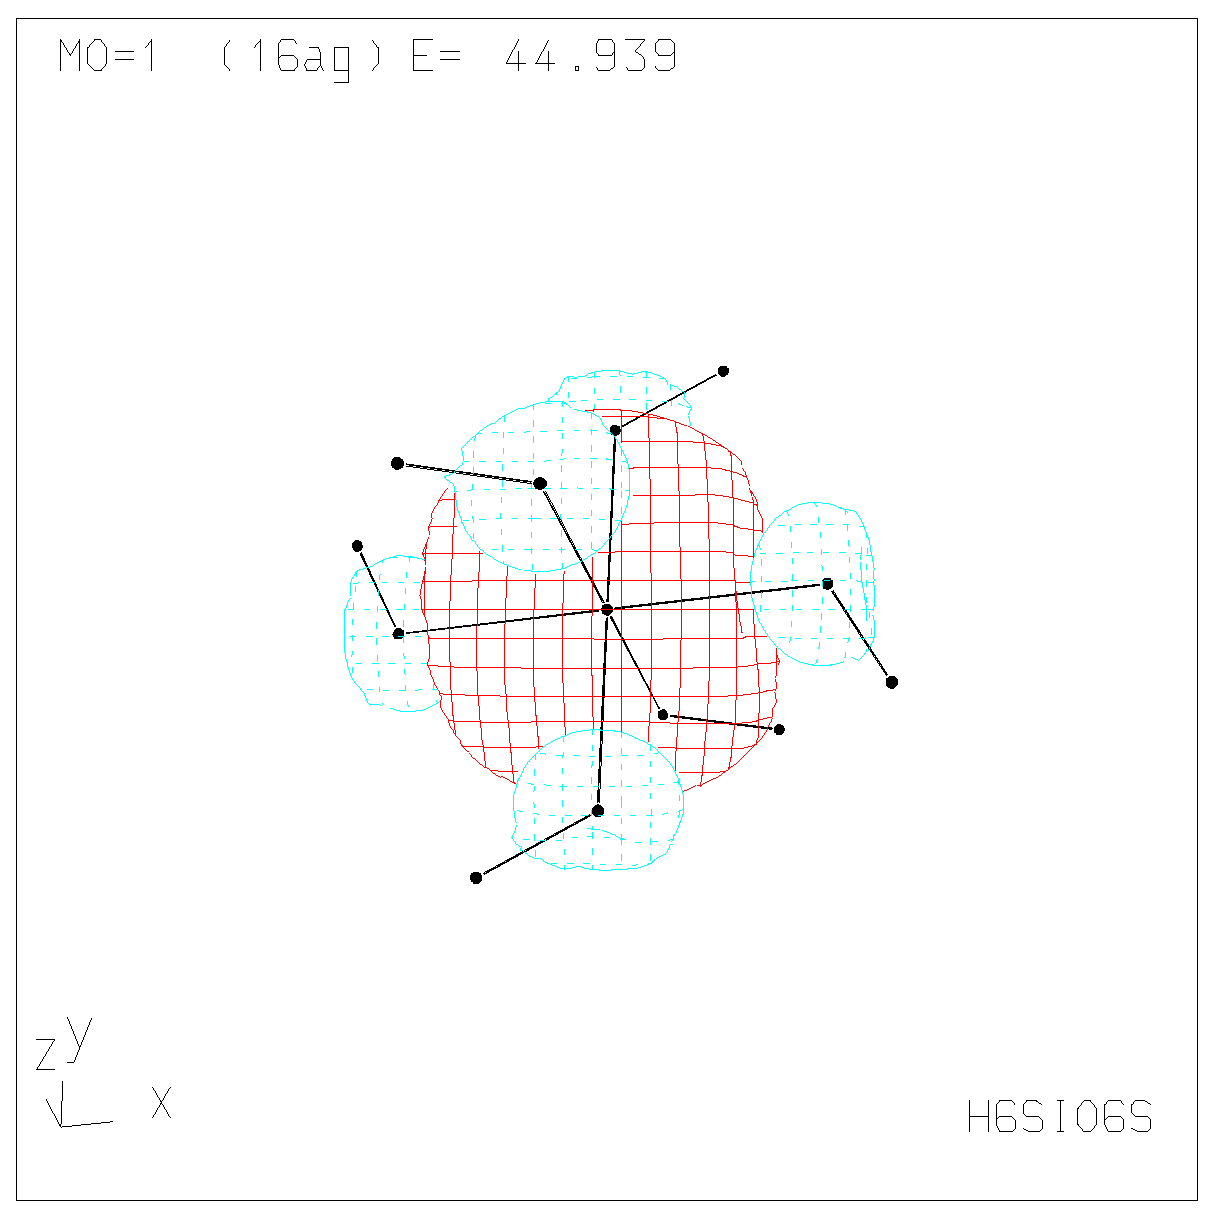
\includegraphics[width=5cm]{h6sio6_obrazky/s1_1.eps} 
\label{obr_h6sio6_MO_s1_1}}
\subfigure[MO 11]{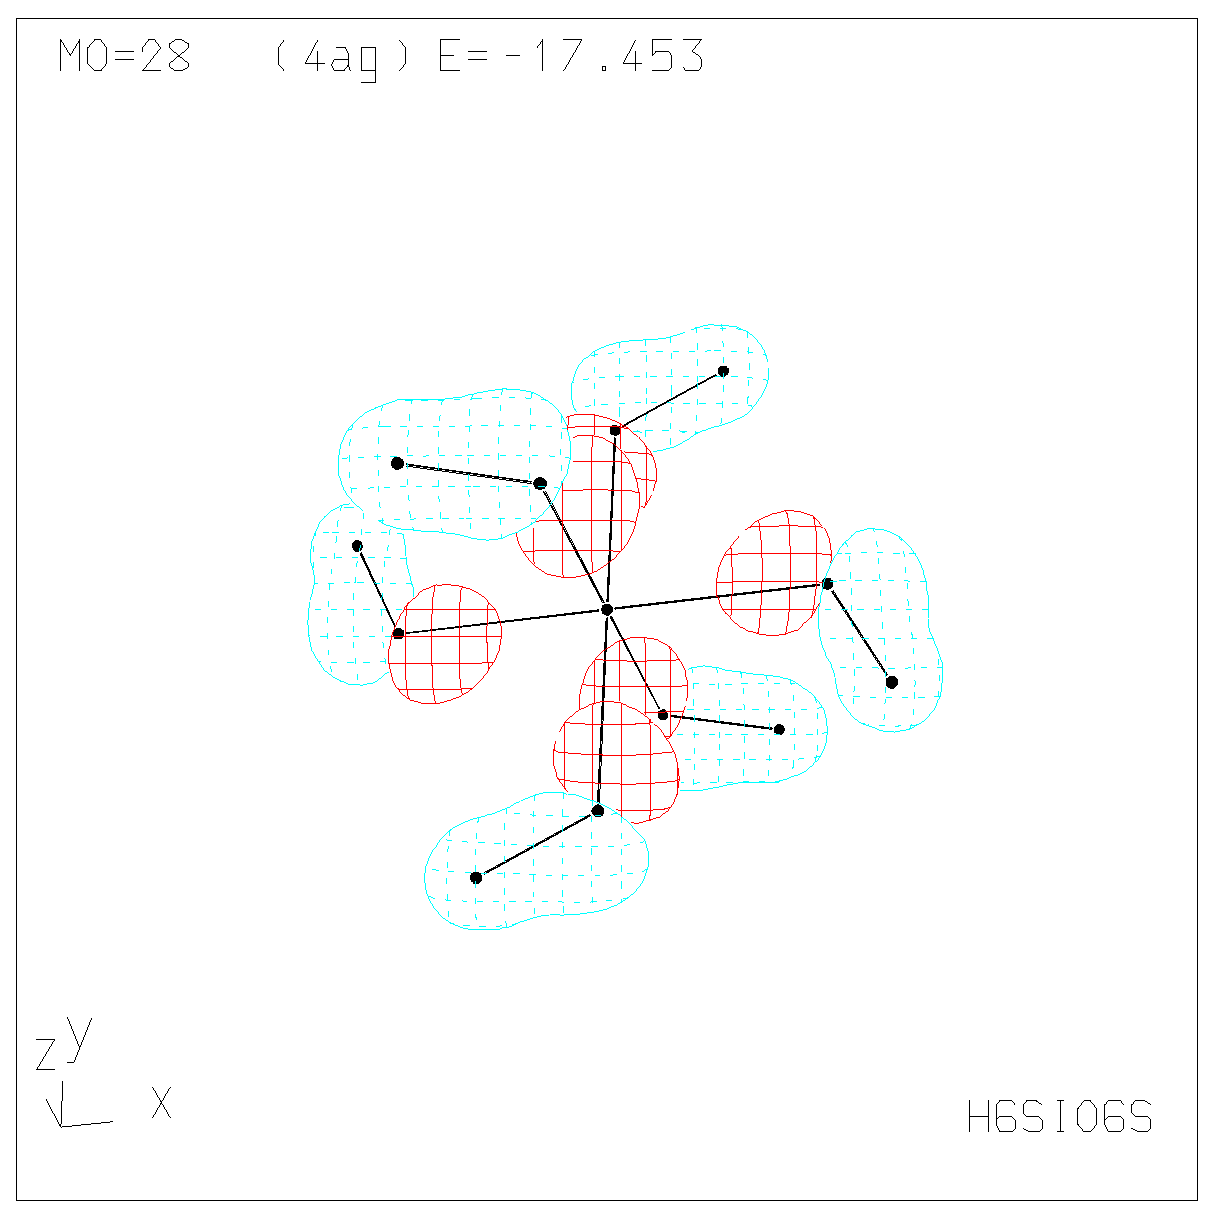
\includegraphics[width=5cm]{h6sio6_obrazky/s1_28.eps}\label{obr_h6sio6_MO_s1_28}}
\subfigure[MO 5]{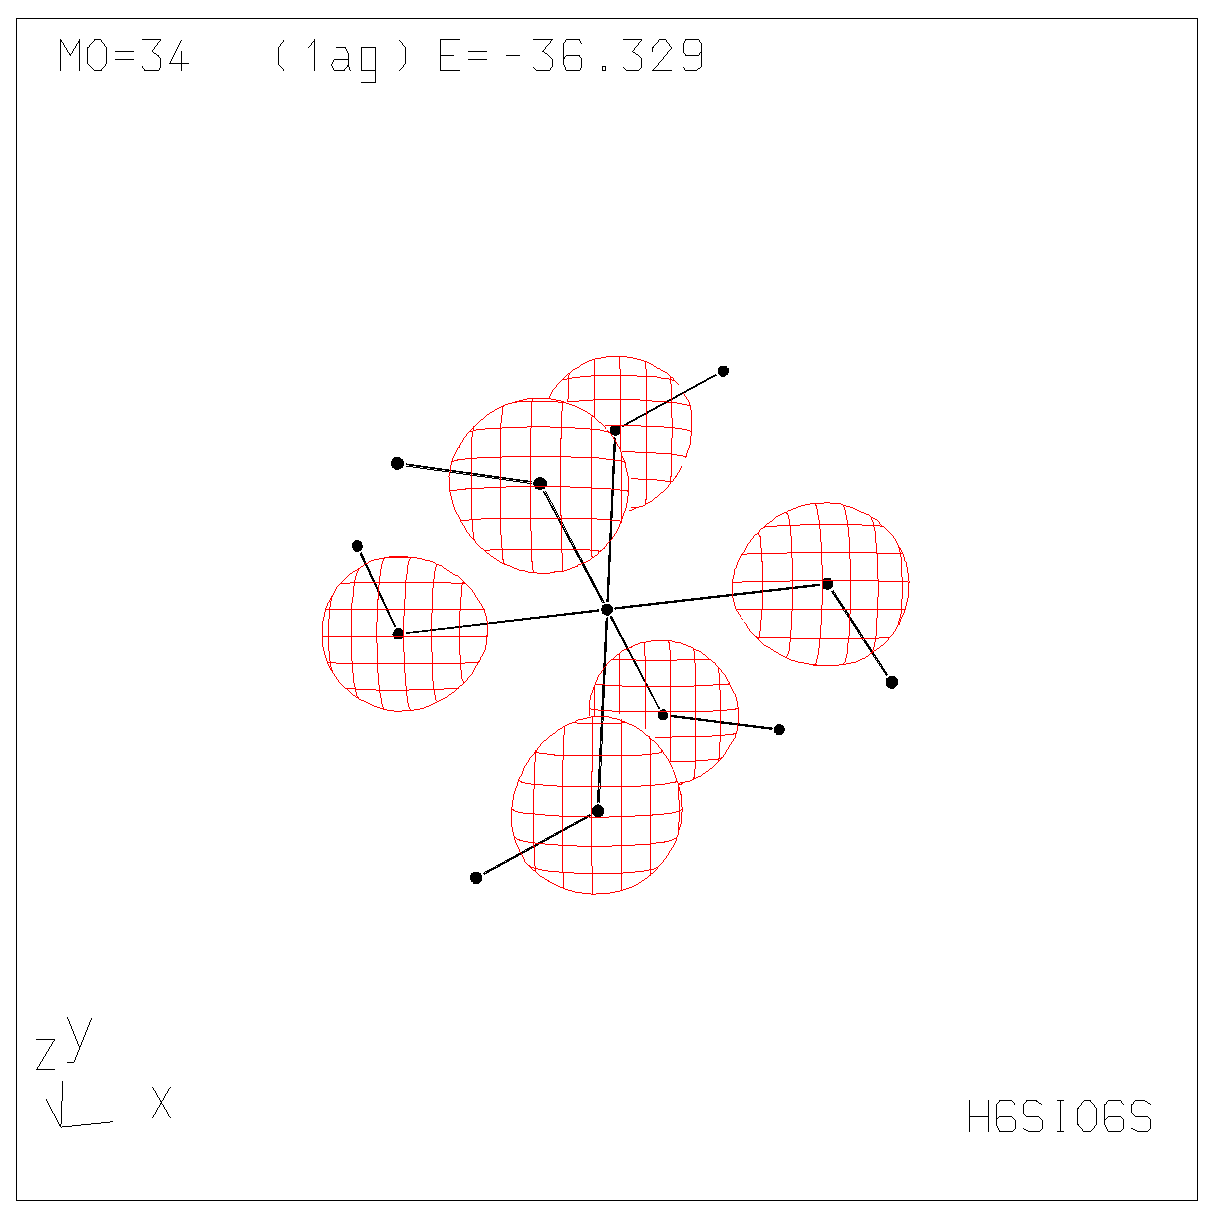
\includegraphics[width=5cm]{h6sio6_obrazky/s1_34.eps} \label{obr_h6sio6_MO_s1_34}}
\caption{Interakce $\bra{30}{\hat{H}}\ket{34}$, $\bra{24}{\hat{H}}\ket{34}$  z tabulky \ref{ttab_h6sio6_vysledky}.}

\label{obr_h6sio6_vysledky_I}\end{center}
\end{figure} 

Fragmentové orbitaly  21, 28 a 32 se navzájem mísí za vzniku MO číslo 3, 26 a 32 znázorněných na obrázku \ref{obr_h6sio6_vysledky_II}.   
\begin{figure}
\begin{center}
\subfigure[MO 3]{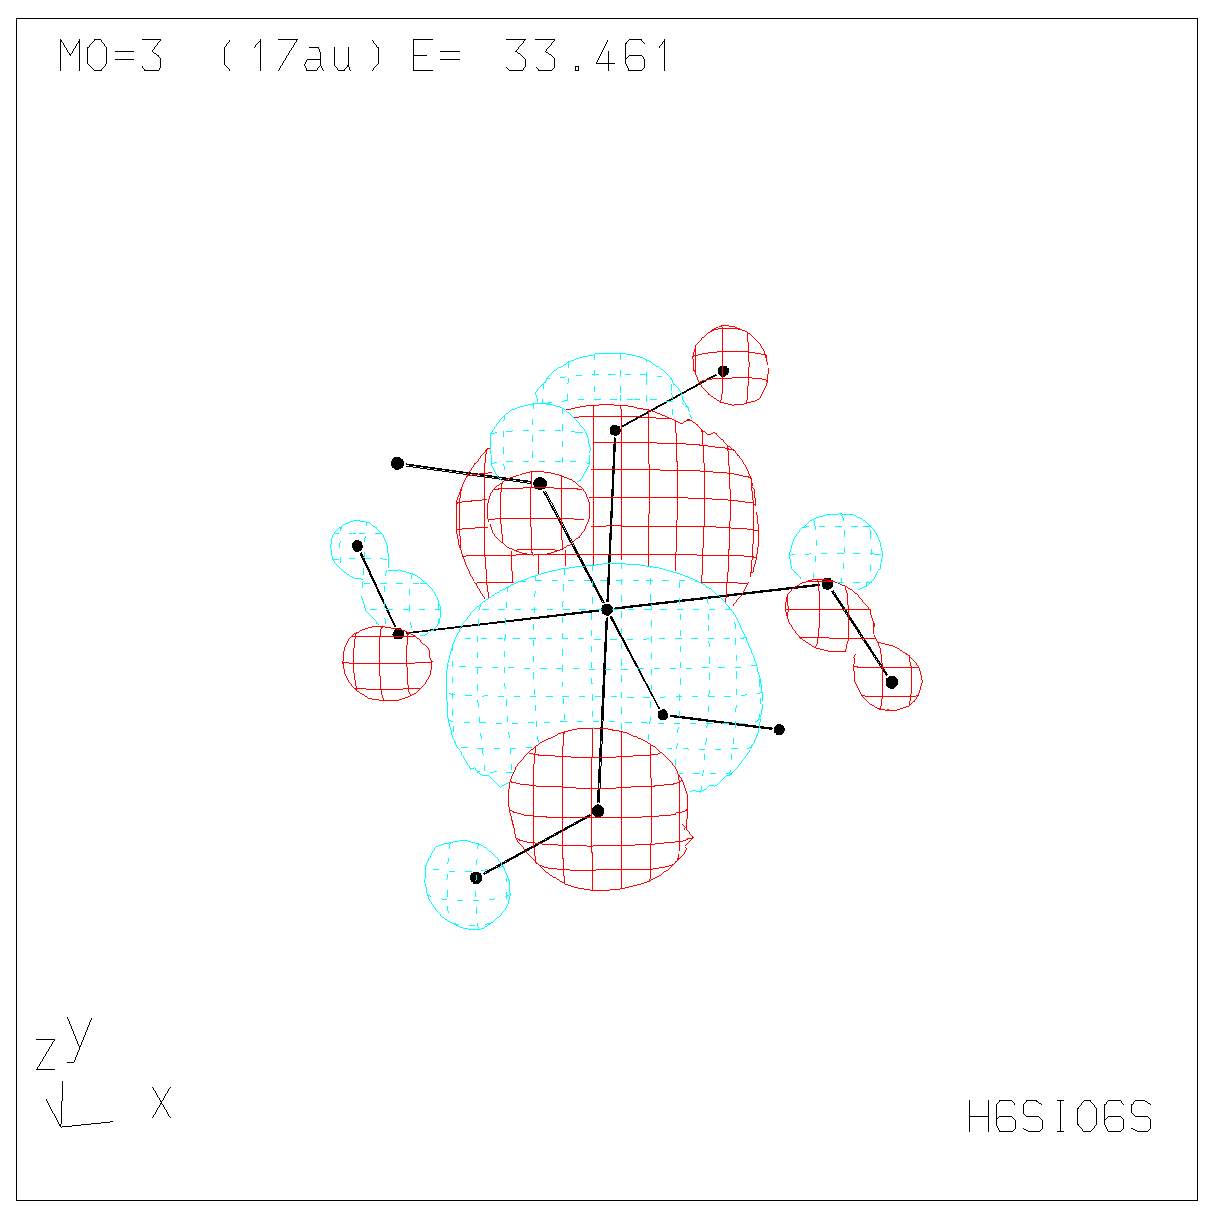
\includegraphics[width=5cm]{h6sio6_obrazky/s2_3.eps} 
\label{obr_h6sio6_MO_s2_3}}
\subfigure[MO 26]{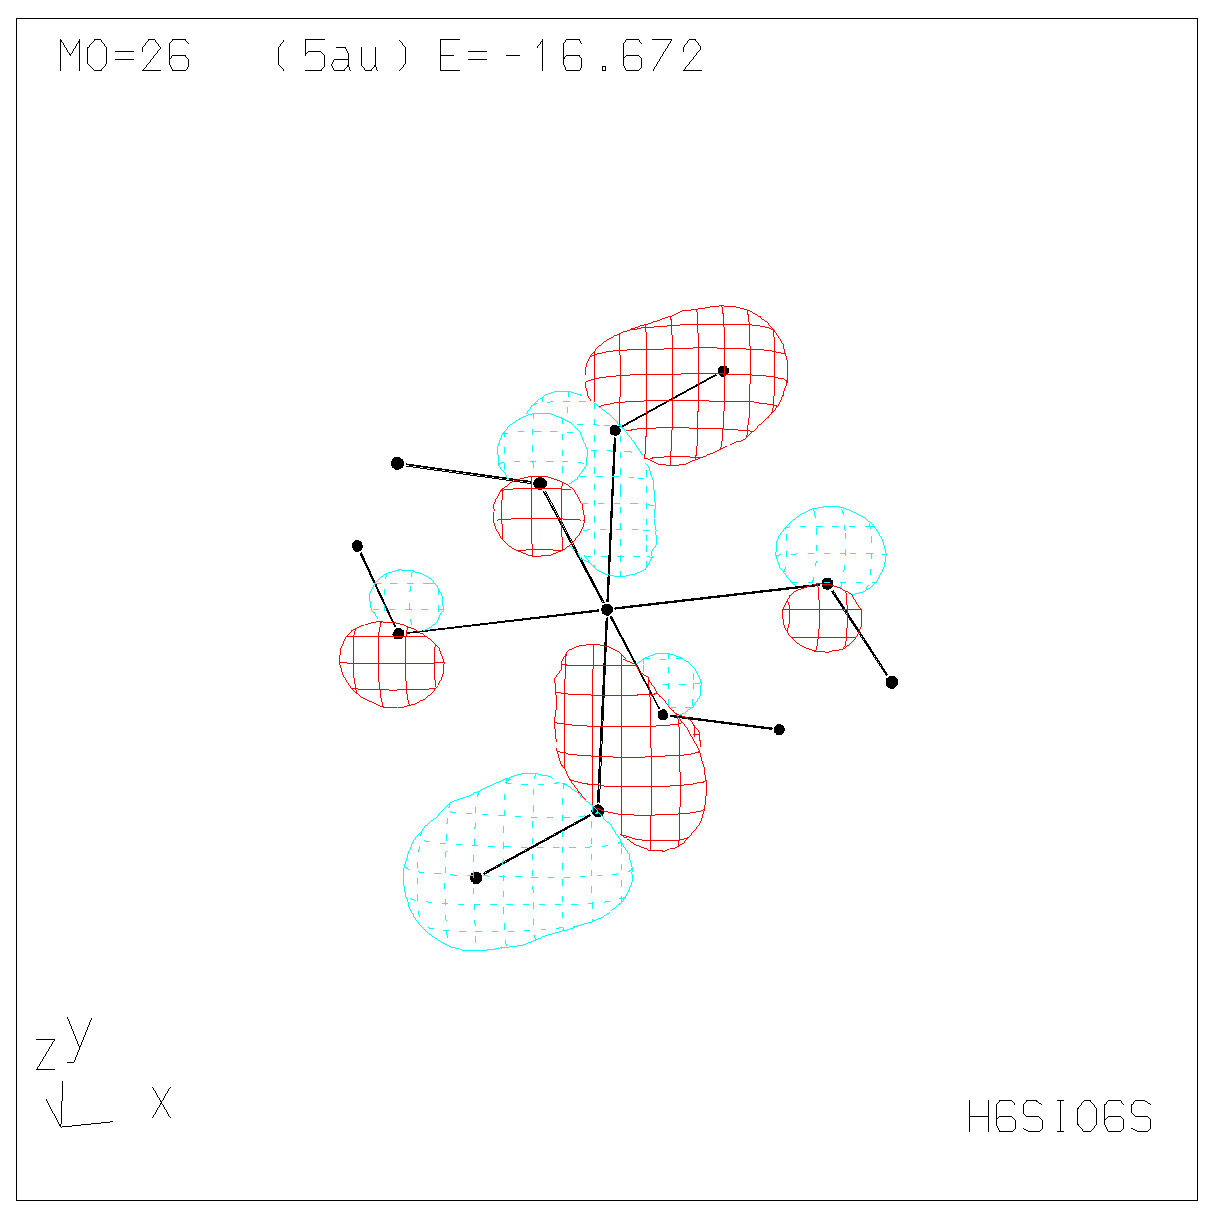
\includegraphics[width=5cm]{h6sio6_obrazky/s2_26.eps}\label{obr_h6sio6_MO_s2_26}}
\subfigure[MO 32]{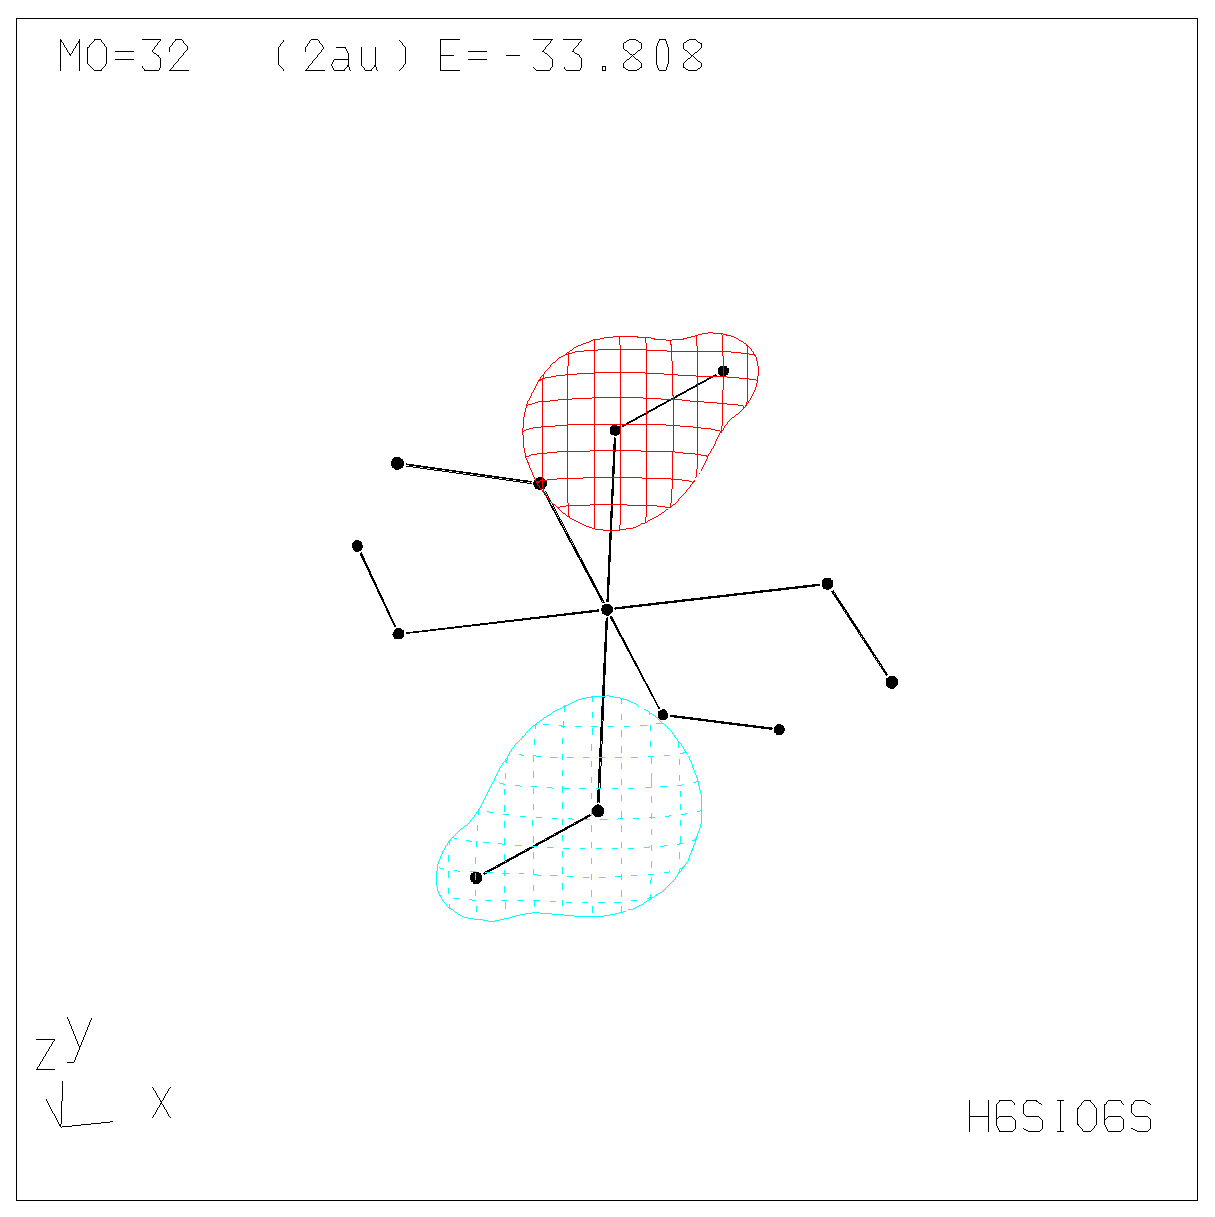
\includegraphics[width=5cm]{h6sio6_obrazky/s2_32.eps} \label{obr_h6sio6_MO_s2_32}}
\caption{Interakce $\bra{21}{\hat{H}}\ket{32}$, $\bra{28}{\hat{H}}\ket{32}$ z tabulky \ref{tab_h6sio6_vysledky}.}

\label{obr_h6sio6_vysledky_II}\end{center}
\end{figure} 
 
  Fragmentové orbitaly  22 a 33 se navzájem mísí za vzniku MO číslo 2 znázorněného na obrázku \ref{obr_h6sio6_vysledky_III}.   
\begin{figure}
\begin{center}
\subfigure[MO 2]{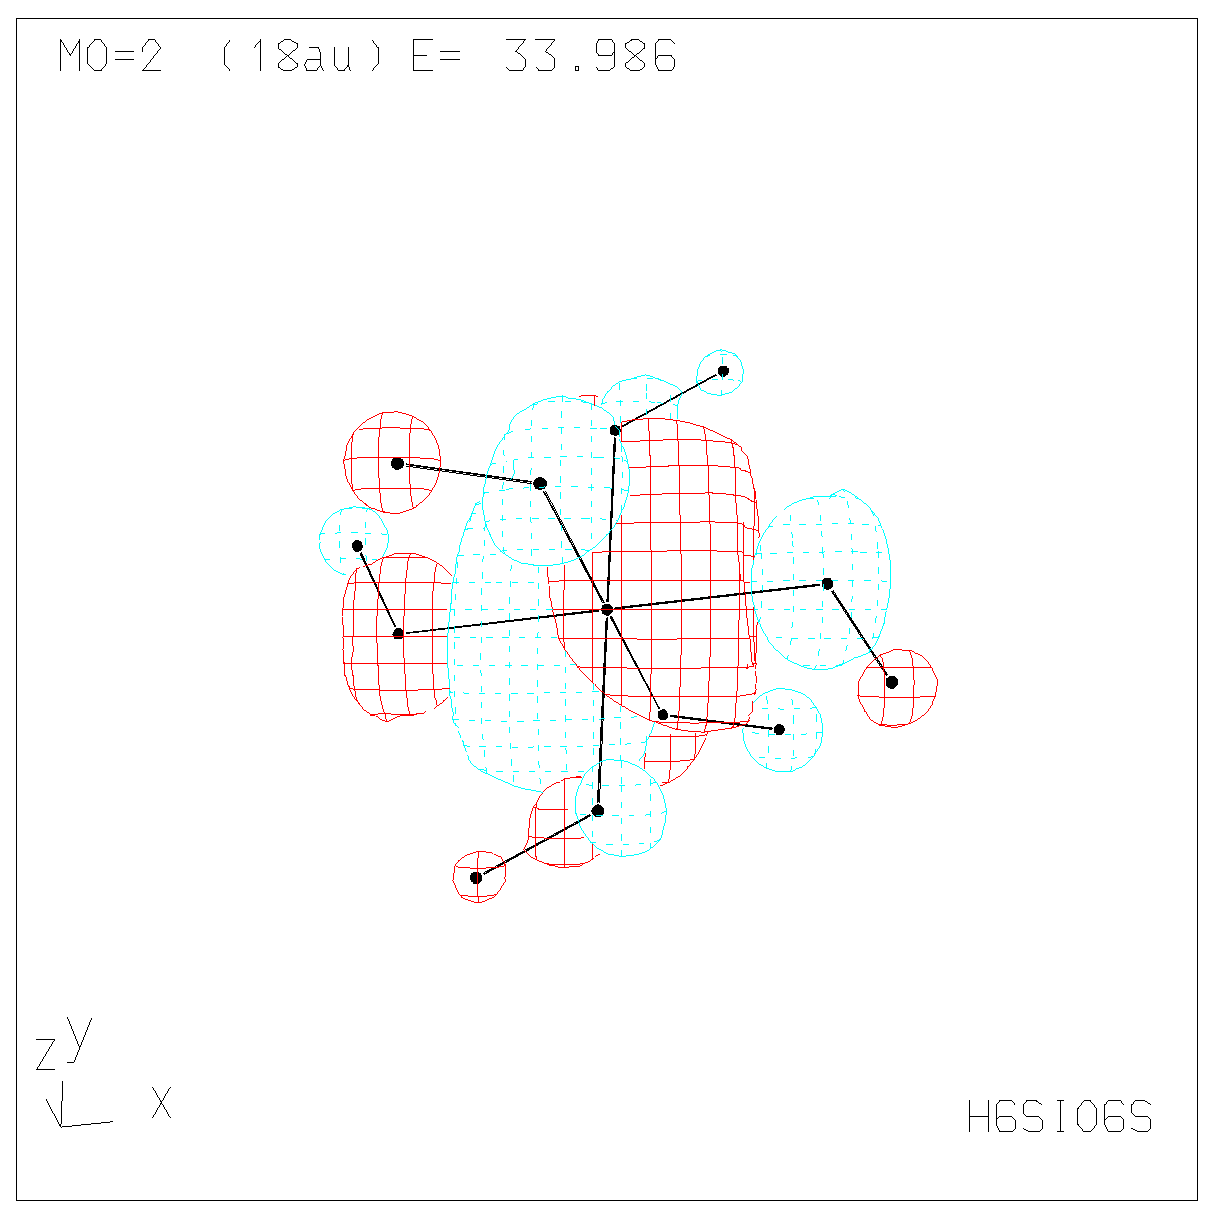
\includegraphics[width=5cm]{h6sio6_obrazky/s3_2.eps} 
\label{obr_h6sio6_MO_s3_2}}
\caption{Interakce $\bra{22}{\hat{H}}\ket{33}$ z tabulky \ref{tab_h6sio6_vysledky}.}

\label{obr_h6sio6_vysledky_III}\end{center}
\end{figure} 
%----------------------------------------------------------------------------------------
 \subsection{Molekula Si(OH)$_3$O(H$_2$PO$_3$)}
 Pro molekulu \ce{Si(OH)3O(H2PO3)} \ref{obr_h3sio4_h2po3} byla nutná oprava zvolených fragmentů vzhledem k výpočetní náročnosti. Jako fragment jedna byla zvolena část \ce{Si(OH)3} a fragment dva byl \ce{O(H2PO3)}.  

  \begin{figure}[h]
\caption{Optimalizovaná struktura \ce{H3SiO4(H2PO3)} }
  \center
  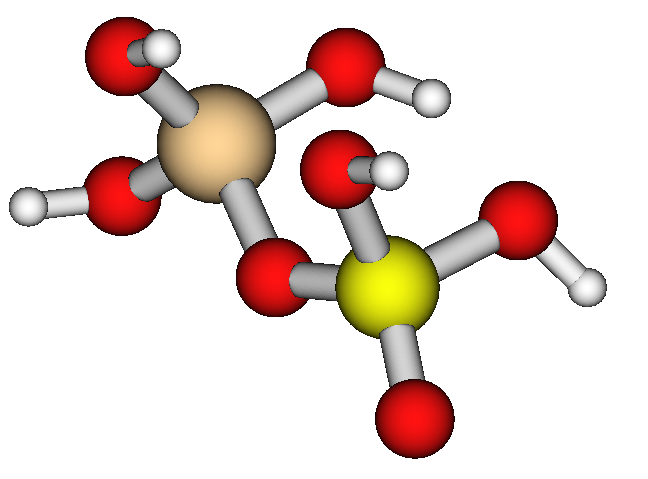
\includegraphics[width=10cm]{obr_h3sio4_h2po3.png}
  \label{obr_h3sio4_h2po3}
  \end{figure}

\begin{table}[htbp]
\caption{Výsledné mísení orbitalů pro  \ce{Si(OH)3O(H2PO3)}}
\begin{center}
\begin{tabular}{|r|r|}
\hline
\multicolumn{2}{|c|}{$\bra{19}{\hat{H}}\ket{29}$, $\bra{15}{\hat{H}}\ket{29}$,$\bra{7}{\hat{H}}\ket{29}$, $\bra{22}{\hat{H}}\ket{29}$} \\
\hline \hline
\multicolumn{1}{|l|}{MO} & \multicolumn{1}{r|}{W} \\ \hline
4 & 32 \\ \hline
14 & 73 \\ \hline
30 & 63 \\ \hline
35 & 83 \\ \hline
41 & 46 \\ \hline
\end{tabular}

\label{tab_sio3_vysledky}\end{center}
\end{table}

Fragmentové orbitaly  7, 15, 19, 22 a 29 se navzájem mísí za vzniku MO číslo 4, 14, 30, 35 a 41 znázorněných na obrázku \ref{obr_sio3p_vysledky_I}.   
\begin{figure}
\begin{center}
\subfigure[MO 4]{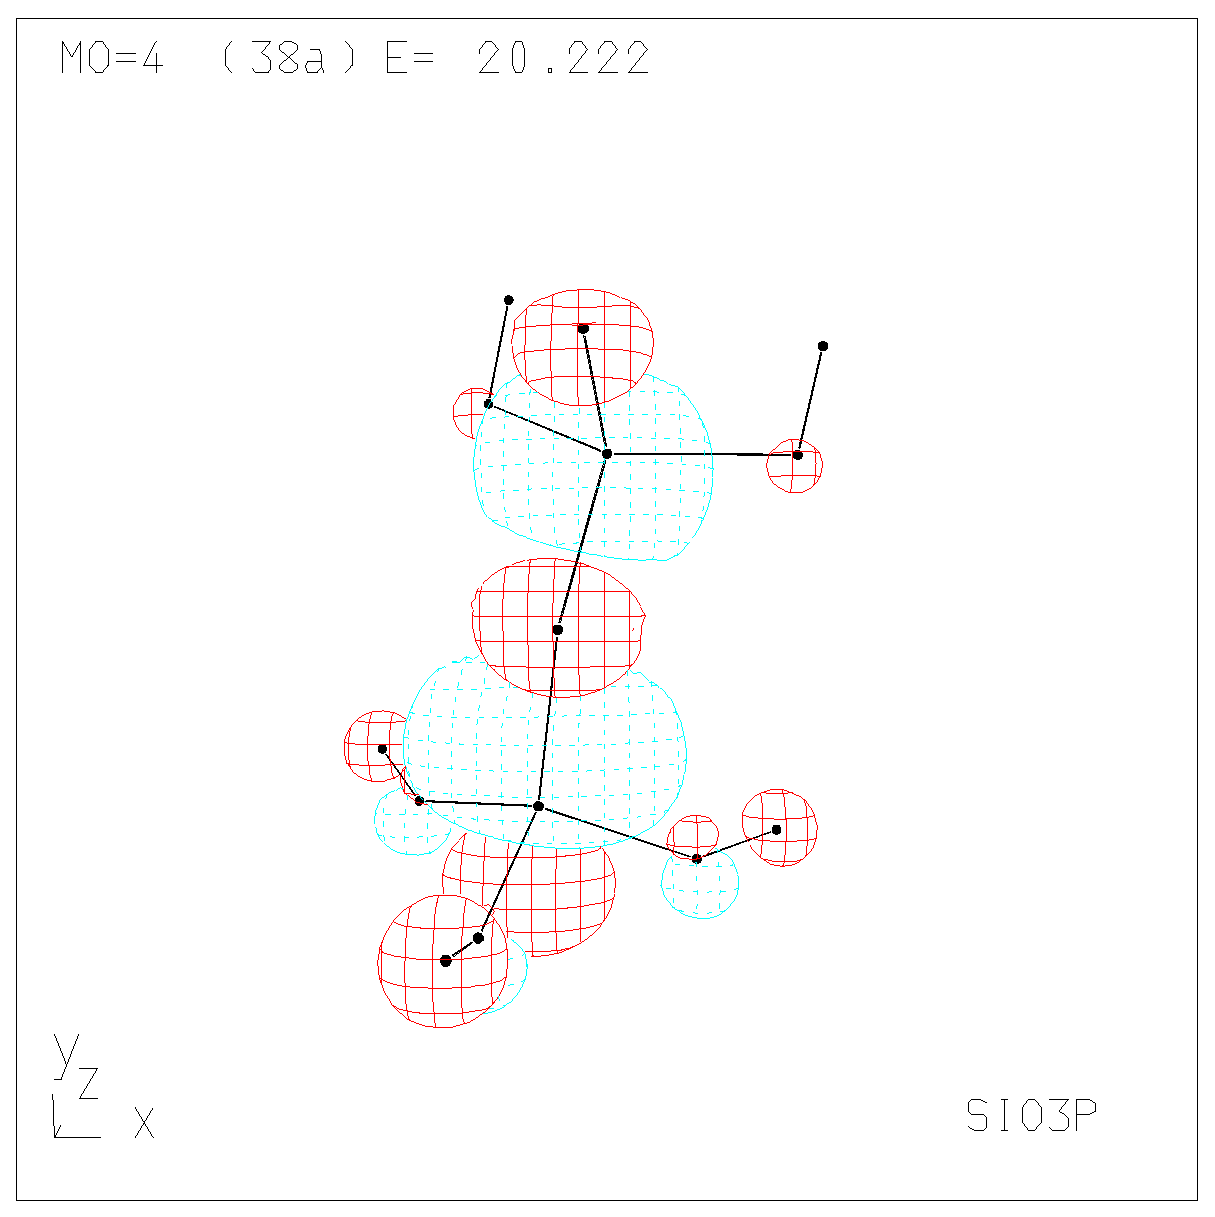
\includegraphics[width=5cm]{sio3p_obrazky/mo_4.eps} 
\label{obr_sio3_MO_4}}
\subfigure[MO 14]{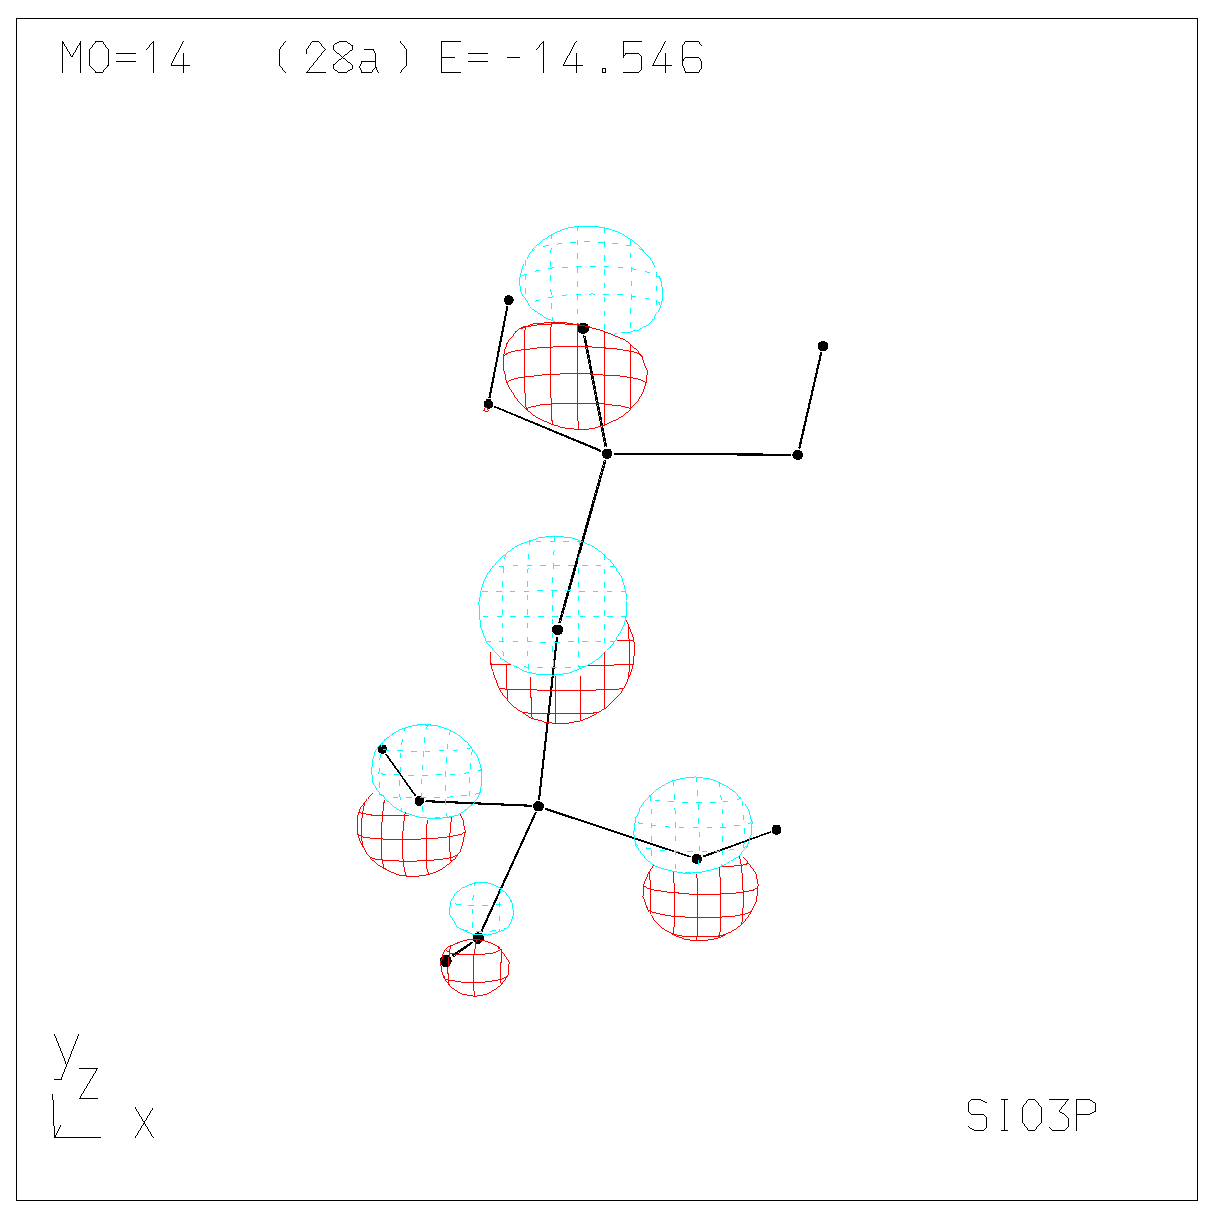
\includegraphics[width=5cm]{sio3p_obrazky/mo_14.eps} 
\label{obr_sio3_MO_14}}
\subfigure[MO 30]{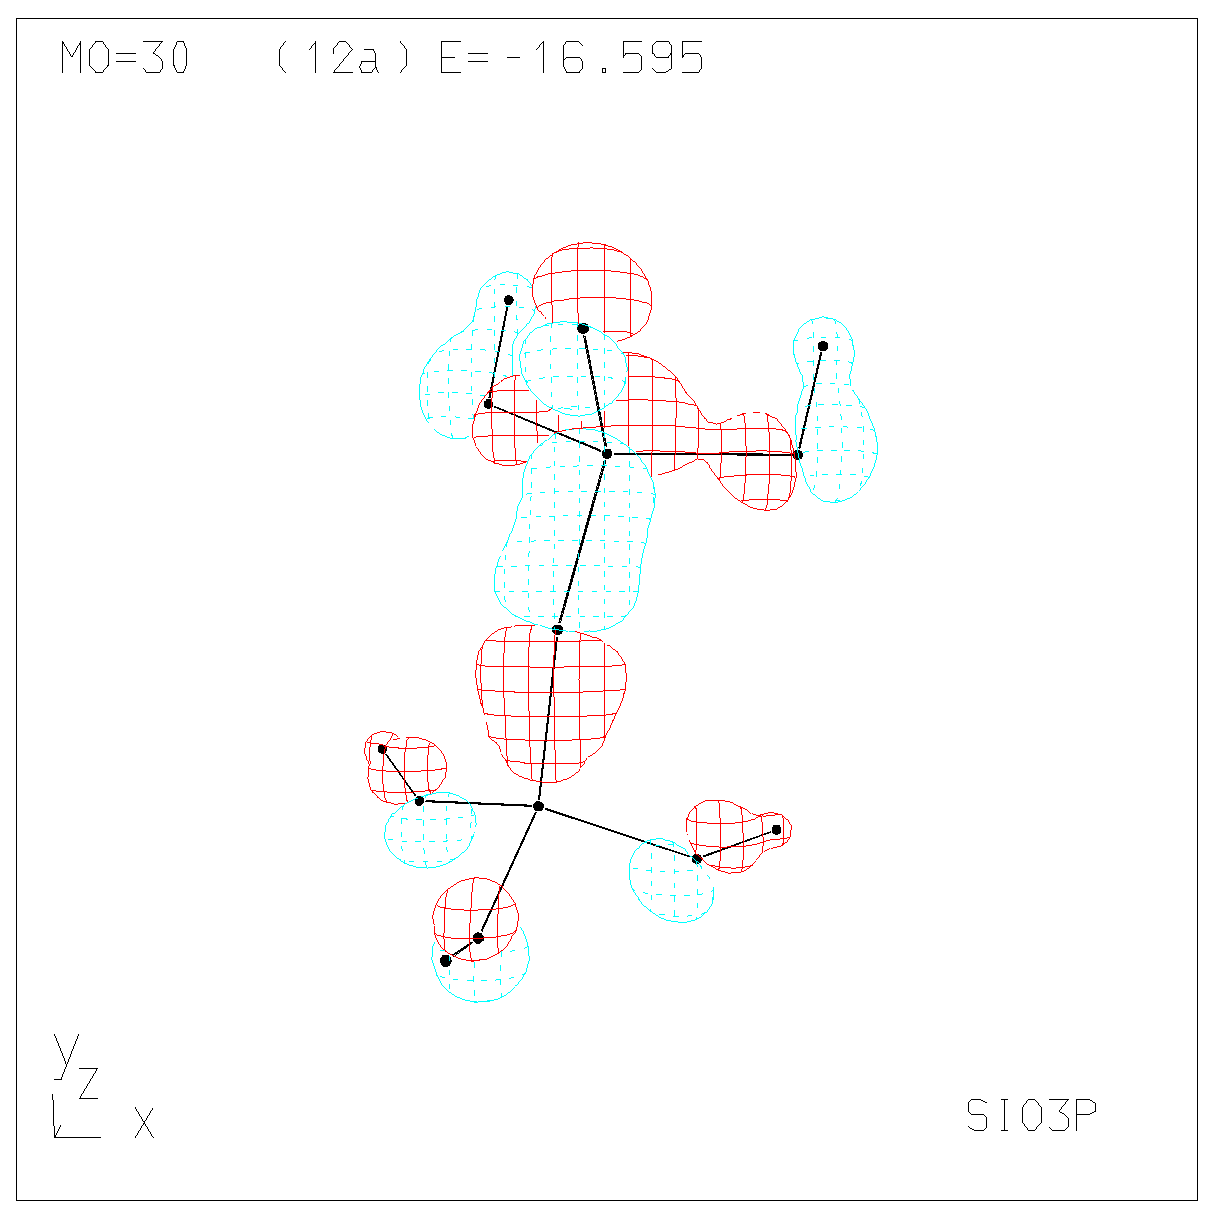
\includegraphics[width=5cm]{sio3p_obrazky/mo_30.eps} 
\label{obr_sio3_MO_30}}
\subfigure[MO 35]{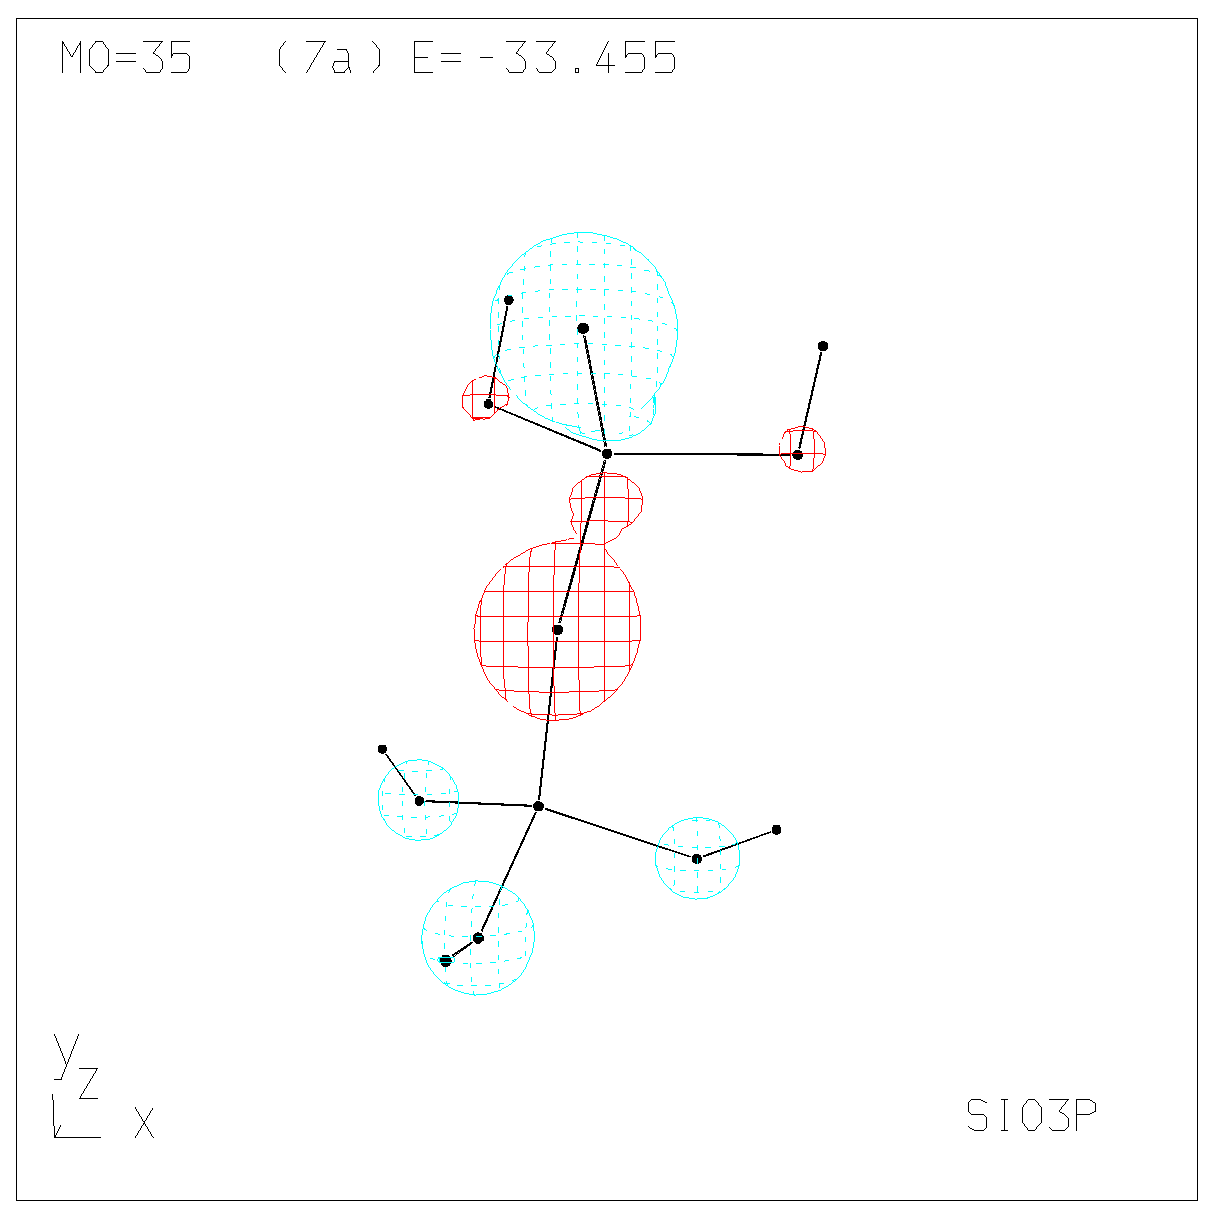
\includegraphics[width=5cm]{sio3p_obrazky/mo_35.eps} 
\label{obr_sio3_MO_35}}
\subfigure[MO 41]{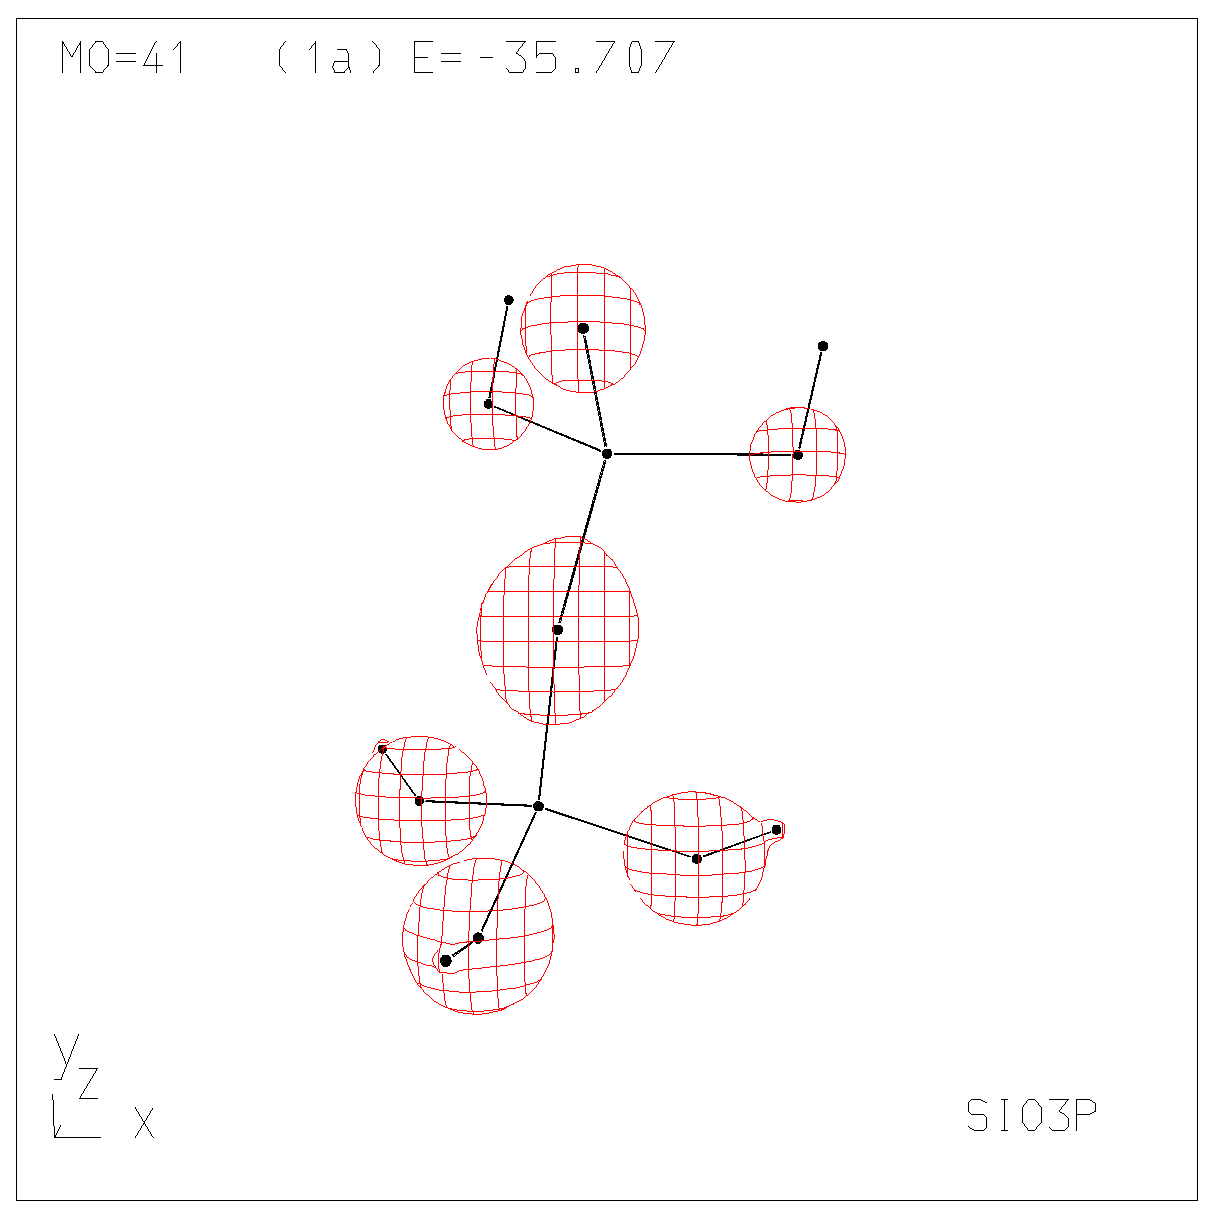
\includegraphics[width=5cm]{sio3p_obrazky/mo_41.eps} 
\label{obr_sio3_MO_41}}
\caption{Interakce $\bra{19}{\hat{H}}\ket{29}$, $\bra{15}{\hat{H}}\ket{29}$,$\bra{7}{\hat{H}}\ket{29}$, $\bra{22}{\hat{H}}\ket{29}$ z tabulky \ref{tab_sio3_vysledky}.}

\label{obr_sio3p_vysledky_I}\end{center}
\end{figure} 
  
\section{DFT výpočet} 
Pro DFT výpočty byly zvoleny molekuly, kde byl Si koordinován šesti kyslíky. Při konstrukci QM modelů molekul se zpočátku vyskytly potíže. Pro systém, kde byl křemík koordinován ve svém okolí šesti fosforečnany, docházelo k umělému vytvoření vodíkových vazeb a sytém se nepodařilo optimalizovat. Z tohoto důvodu bylo nutné použít jako výchozí molekulu křemík koordinovaný šesti fosforečnany, které byly zároveň spojeny jednotkami \ce{SiO4}, viz. obrázek \ref{obr_si_o_poh3_6_propojeno_si}. Další komplikací při optimalizaci geometrické struktury byl celkový náboj molekuly, který byl nakonec určen jako $2-$, viz. výpočet níže. 
\begin{displaymath}
\ce{Si}^{4+} + \ce{(HPO4)^{2-}} + \ce{Si3^{4+}} + \ce{(OH)6^1-} = \ce{Si(HPO4)Si3(OH)6)^{2-}}
\end{displaymath}

\begin{figure}
\begin{center}
\subfigure[	\ce{H4SiO4}]{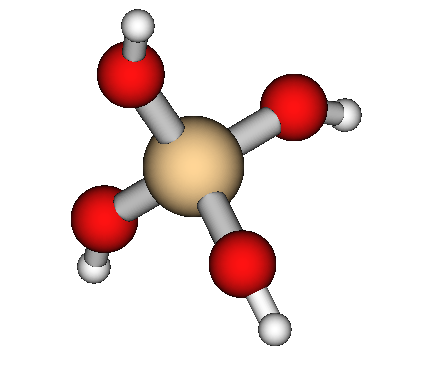
\includegraphics[width=5cm]{h4sio4_obr.png} 
\label{obr_h4sio4_II}}
\subfigure[\ce{(H6SiO6)^{2-}}]{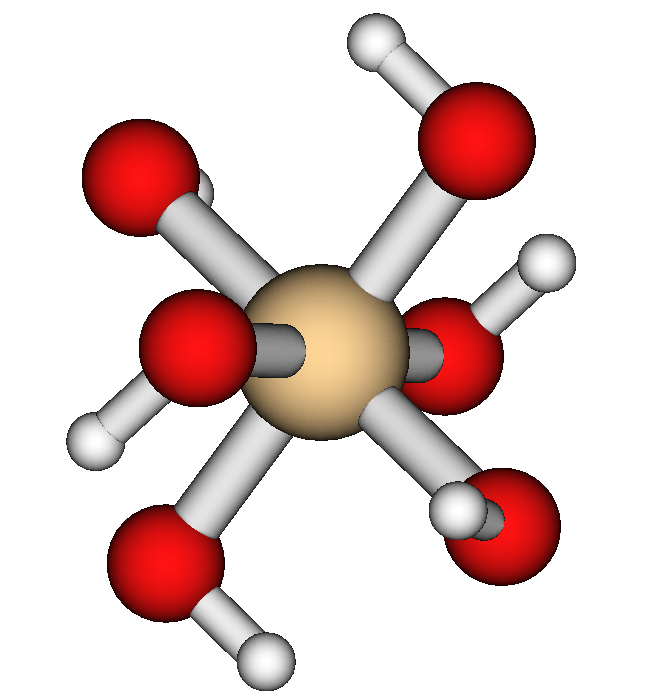
\includegraphics[width=5cm]{obr_h6sio6.png} 
\label{obr_h6sio6_II}}
\subfigure[ \ce{H3SiO3CH3}]{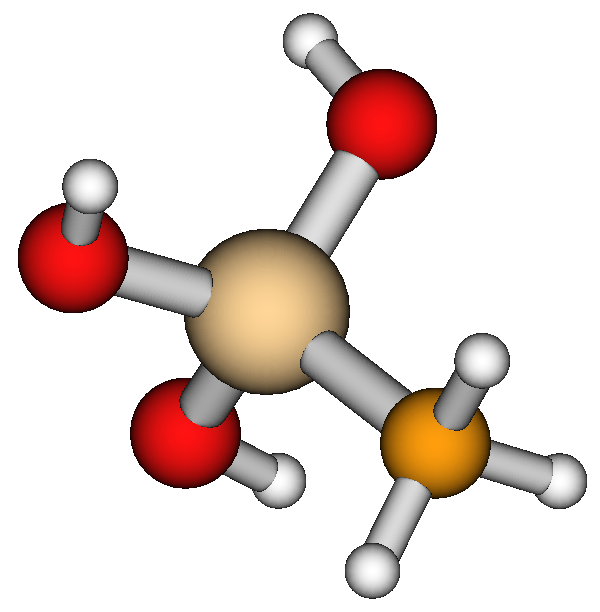
\includegraphics[width=5cm]{si(oh)3ch3_obr.png} 
\label{obr_h3sio3ch3}}
\subfigure[\ce{(H5SiO5CH3)^{2-}} ]{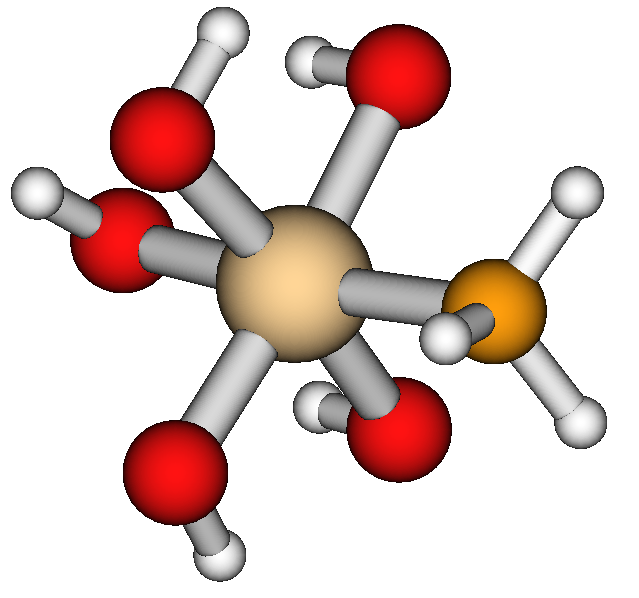
\includegraphics[width=5cm]{obr_h5sio5ch3.png} 
\label{obr_h5sio5ch3}}
\subfigure[\ce{H3SiO4(H2PO3)}]{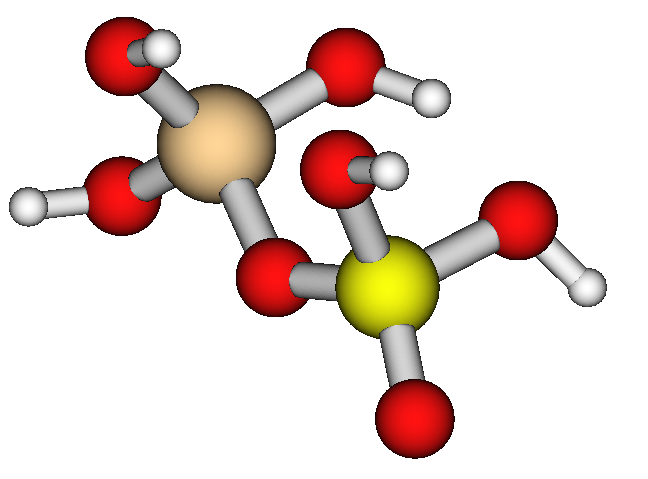
\includegraphics[width=5cm]{obr_h3sio4_h2po3.png} 
\label{obr_h3sio4_h2po3}}
\subfigure[\ce{SiO4(H2PO3)4}]{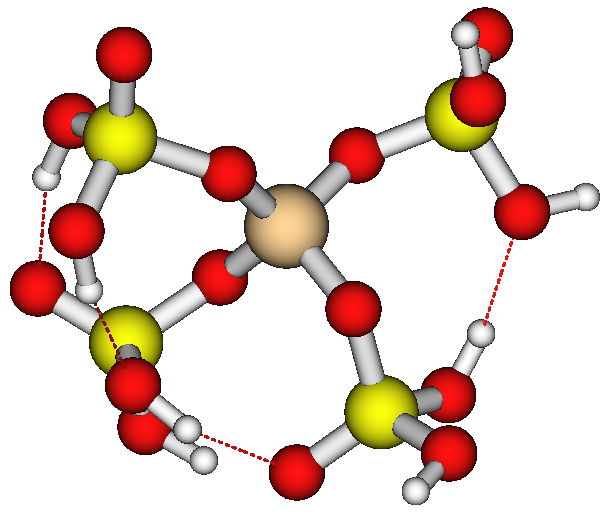
\includegraphics[width=5cm]{obr_sio4_h2po3_4.png} 
\label{obr_sio4_h2po3_4}}
\caption{Optimalizované struktury sloučenin křemíku}
\label{tab_vysledky_dft_I}\end{center}
\end{figure} 

\begin{figure}
\begin{center}
\subfigure[\ce{(SiO6(H2PO3)6(SiO4)6)^{2-}}]{\includegraphics[width=5cm]{obr_si_kryst_struktura.png} 
\label{obr_sobr_si_kryst_struktura}}
\subfigure[\ce{(Si^{VI}(PO4)6(Si^{IV}O4Et2)6)^{2-}} ]{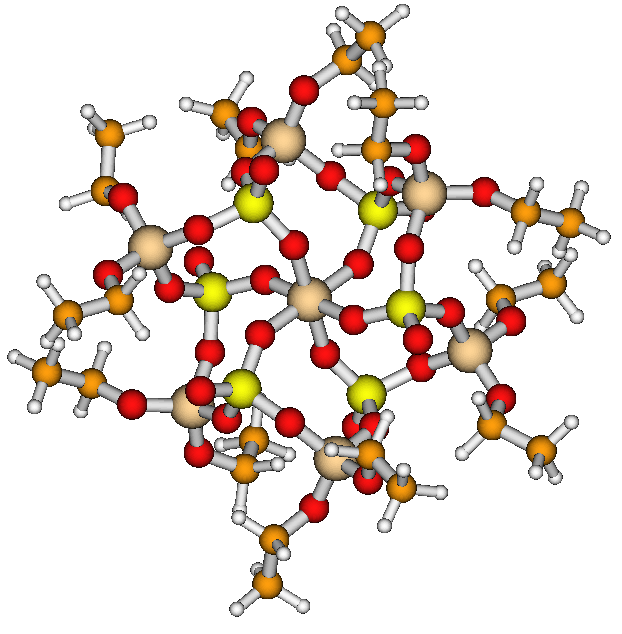
\includegraphics[width=5cm]{obr_si_kryst_struktura_real.png} 
\label{obr_si_kryst_struktura_real}}
\subfigure[\ce{Si(PO4)4(C2CH3)2(Si(OH)2)6}]{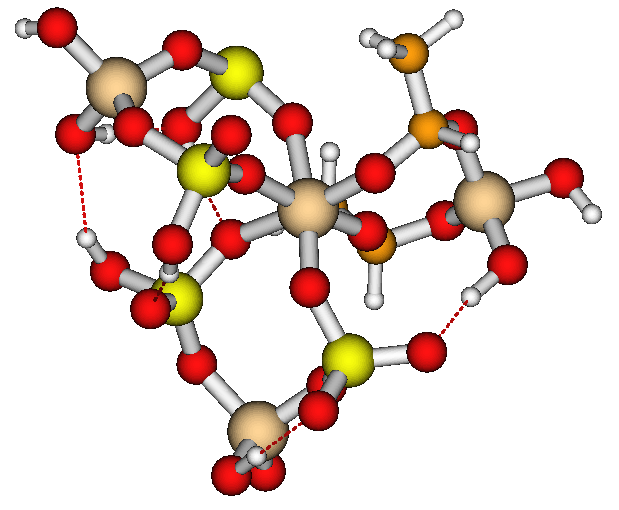
\includegraphics[width=5cm]{obr_si_o_poh_propojeno_si_jeden_kruh.png} 
\label{obr_si_o_poh3_6_propojeno_si}}
\subfigure[\ce{Si(PO4)4(C2CH3)2(Si(OH)2)6}]{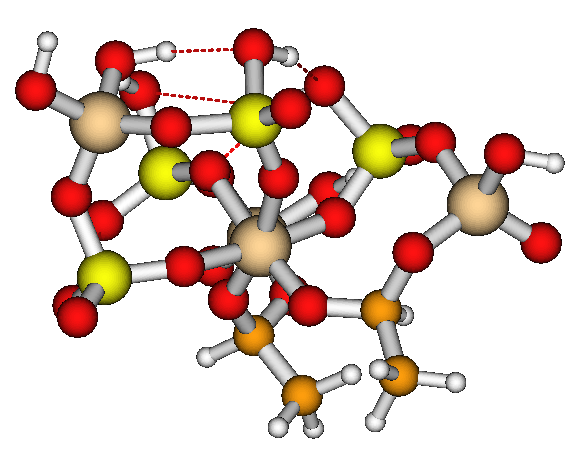
\includegraphics[width=5cm]{obr_sipo4_4_ax_ekv.png} 
\label{obr_sipo4_4_ax_ekv}}
\caption{Optimalizované struktury křemičitofosfátů}
\end{center}
\end{figure}

\begin{table}[htbp]
\begin{minipage}{\textwidth}
\caption{Srovnání energiových parametrů pro vybrané struktury}
\begin{center}
\begin{tabular}{|l|r|r|r|r|}
\hline
 & E$_{\ce{H}}$\footnote{HOMO $-$ Highest Occupied Molecular Orbital} [eV] & E$_{\ce{L}}$ \footnote{LUMO$ - $Lowest Unoccupied Molecular Orbital} [eV]& $\chi$ [eV] & $\eta$ [eV] \\ \hline
\hline
\ce{H4SiO4}  & -7,730 & 1,677 & 9,407 & 6,053 \\ \hline
\ce{(H6SiO6)^{2-}}  & 3,610 & 11,697 & 8,087 & -15,307 \\ \hline
\ce{H3SiO3CH3}  & -7,750 & 0,825 & 8,575 & 6,925 \\ \hline
\ce{(H5SiO5CH3)^{2-}}  & 3,883 & 11,550 & 7,667 & -15,433 \\ \hline
\ce{H3SiO4(H2PO3)} & -8,567 & 0,060 & 8,627 & 8,507 \\ \hline
\ce{SiO4(H2PO3)} & -8,088 & -0,829 & 7,259 & 8,917 \\ \hline
\ce{(SiO6(H2PO3)6)^{2-}} & - \footnote{Strukturu se nepodařilo optimalizovat z důvodu nestability}& - & -& - \\ \hline
\ce{Si(H2PO3)3OH} & - \footnote{Strukturu se nepodařilo optimalizovat z důvodu tvorby umělých vodíkových můstků} & - & - & - \\ \hline
\ce{(Si(H2PO3)5OH)^{2-}} & - \footnote{Strukturu se nepodařilo optimalizovat z důvodu nestability} & - & - & - \\ \hline
\ce{(Si(PO4)6(Si(OH)2)6)^{2-}} \footnote{Optimalizace s bazí IGLO-III} & -3,670 & 4,040 & 7,710 & -0,369 \\ \hline
\ce{(Si(PO4)6(Si(OH)2)6)^{2-}} \footnote{Optimalizace s bazí 6-31G*}& -3,346 & 4,574 & 7,718 & -2,501 \\ \hline
\ce{Si^{VI}(PO4)6(Si^{IV}O4Et2)6}\footnote{VI a IV jsou hodnoty koordinace křemíku, zdroj \cite{C3NJ00721A}} & -2,609 & 5,109 & 7,718& -2,501 \\ \hline
\ce{Si(PO4)4(C2CH3)2(Si(OH)2)6} \footnote{Fosfor je nahrazen uhlíkem v rámci jednoho kruhu}& 5,366 & 10,467 & 5,101 & -15,833 \\ \hline
\ce{(Si(PO4)4(C2CH3)2(Si(OH)2)6)^{4-}} \footnote{Fosfor je nahrazen uhlíkem na dvou různých kruzích} & 5,081 & 10,138 & 5,057 & -15,219 \\ \hline
\end{tabular}
\end{center}
\label{tab_porovnani_molekul_dft}
\end{minipage}
\end{table}

\begin{table}[htbp]
\begin{minipage}{\textwidth}
%\caption{Výsledky pro absolutní magnetické stínění}
\begin{center}
\begin{tabular}{|r|r|r|}
\hline
\multicolumn{1}{|l|}{Ćíslo atomu} & \multicolumn{1}{l|}{Abs. magn. stínění [ppm]} & \multicolumn{1}{l|}{Chem. posuv \footnote{Experimentální hodnoty \cite{1316862}} [ppm]} \\ \hline
1 & 546,5 & -101 \\ \hline
43 & 433,0 & -212 \\ \hline
44 & 432,9 & -212 \\ \hline
45 & 432,1 & -212 \\ \hline
46 & 432,9 & -212 \\ \hline
47 & 432,9 & -212 \\ \hline
48 & 432,3 & -212 \\ \hline
\end{tabular}
\end{center}
\label{vysledky_abs_magn_stineni}
\end{minipage}
\end{table}

  
  
{\csname captions\languagename\endcsname %% Temporarily override
%% the BibLaTeX localization with the original babel definitions.
\makeatletter %% Use the correct localization of the quotations.
  \thesis@selectLocale{\thesis@locale}\makeatother
\printbibliography[heading=bibintoc]} %% Print the bibliography.
\appendix %% Start the appendices.
\chapter{An appendix}
Here you can insert the appendices of your thesis.   




\end{document}
